\documentclass{book}
\usepackage[a4paper,top=2.5cm,bottom=2.5cm,left=2.5cm,right=2.5cm]{geometry}
\usepackage{makeidx}
\usepackage{natbib}
\usepackage{graphicx}
\usepackage{multicol}
\usepackage{float}
\usepackage{listings}
\usepackage{color}
\usepackage{ifthen}
\usepackage[table]{xcolor}
\usepackage{textcomp}
\usepackage{alltt}
\usepackage{ifpdf}
\ifpdf
\usepackage[pdftex,
            pagebackref=true,
            colorlinks=true,
            linkcolor=blue,
            unicode
           ]{hyperref}
\else
\usepackage[ps2pdf,
            pagebackref=true,
            colorlinks=true,
            linkcolor=blue,
            unicode
           ]{hyperref}
\usepackage{pspicture}
\fi
\usepackage[utf8]{inputenc}
\usepackage{mathptmx}
\usepackage[scaled=.90]{helvet}
\usepackage{courier}
\usepackage{sectsty}
\usepackage[titles]{tocloft}
\usepackage{doxygen}
\lstset{language=C++,inputencoding=utf8,basicstyle=\footnotesize,breaklines=true,breakatwhitespace=true,tabsize=8,numbers=left }
\makeindex
\setcounter{tocdepth}{3}
\renewcommand{\footrulewidth}{0.4pt}
\renewcommand{\familydefault}{\sfdefault}
\hfuzz=15pt
\setlength{\emergencystretch}{15pt}
\hbadness=750
\tolerance=750
\begin{document}
\hypersetup{pageanchor=false,citecolor=blue}
\begin{titlepage}
\vspace*{7cm}
\begin{center}
{\Large S\-N\-A\-P }\\
\vspace*{1cm}
{\large Generated by Doxygen 1.8.1.1}\\
\vspace*{0.5cm}
{\small Wed Mar 20 2013 13:01:00}\\
\end{center}
\end{titlepage}
\clearemptydoublepage
\pagenumbering{roman}
\tableofcontents
\clearemptydoublepage
\pagenumbering{arabic}
\hypersetup{pageanchor=true,citecolor=blue}
\chapter{R\-E\-A\-D\-M\-E.\-md}
\label{index}\hypertarget{index}{}\section*{S\-N\-A\-P\-: S\-N (Discrete Ordinates) Application Proxy}

\subsection*{Description}

S\-N\-A\-P serves as a proxy application to model the performance of a modern discrete ordinates neutral particle transport application. S\-N\-A\-P may be considered an update to \href{http://www.ccs3.lanl.gov/PAL/software.shtml}{\tt Sweep3\-D}, intended for hybrid computing architectures. It is modeled off the Los Alamos National Laboratory code P\-A\-R\-T\-I\-S\-N. P\-A\-R\-T\-I\-S\-N solves the linear Boltzmann transport equation (T\-E), a governing equation for determining the number of neutral particles (e.\-g., neutrons and gamma rays) in a multi-\/dimensional phase space. S\-N\-A\-P itself is not a particle transport application; S\-N\-A\-P incorporates no actual physics in its available data, nor does it use numerical operators specifically designed for particle transport. Rather, S\-N\-A\-P mimics the computational workload, memory requirements, and communication patterns of P\-A\-R\-T\-I\-S\-N. The equation it solves has been composed to use the same number of operations, use the same data layout, and load elements of the arrays in approximately the same order. Although the equation S\-N\-A\-P solves looks similar to the T\-E, it has no real world relevance.

The solution to the time-\/dependent T\-E is a \char`\"{}flux\char`\"{} function of seven independent variables\-: three spatial (3-\/\-D spatial mesh), two angular (set of discrete ordinates, directions in which particles travel), one energy (particle speeds binned into \char`\"{}groups\char`\"{}), and one temporal. P\-A\-R\-T\-I\-S\-N, and therefore S\-N\-A\-P, uses domain decomposition over these dimensions to coherently distribute the data and the tasks associated with solving the equation. The parallelization strategy is expected to be the most efficient compromise between computing resources and the iterative strategy necessary to converge the flux.

The iterative strategy is comprised of a set of two nested loops. These nested loops are performed for each step of a time-\/dependent calculation, wherein any particular time step requires information from the preceding one. No parallelization is performed over the temporal domain. However, for time-\/dependent calculations two copies of the unknown flux must be stored, each copy an array of the six remaining dimensions. The outer iterative loop involves solving for the flux over the energy domain with updated information about coupling among the energy groups. Typical calculations require tens to hundreds of groups, making the energy domain suitable for threading with the node's (or nodes') provided accelerator. The inner loop involves sweeping across the entire spatial mesh along each discrete direction of the angular domain. The spatial mesh may be immensely large. Therefore, S\-N\-A\-P spatially decomposes the problem across nodes and communicates needed information according to the K\-B\-A method. K\-B\-A is a transport-\/specific application of general parallel wavefront methods. Lastly, although K\-B\-A efficiency is improved by pipelining operations according to the angle, current chipsets operate best with vectorized operations. During a mesh sweep, S\-N\-A\-P operations are vectorized over angles to take advantage of the modern hardware.

S\-N\-A\-P should be tested with problem sizes that accurately reflect the types of calculations P\-A\-R\-T\-I\-S\-N frequently handles. The spatial domain shall be decomposed to 2,000--4,000 cells per node (M\-P\-I rank). Each node will own all the energy groups and angles for that group of cells; typical calculations feature 10--100 energy groups and as few as 100 to as many as 2,000 angles. Moreover, sufficient memory must be provided to store two full copies of the solution vector for time-\/dependent calculations. The preceding parameters assume current trends in available per core memory. Significant advances or detriments affecting this assumption shall require reconsideration of appropriate parameters per compute node.

\subsection*{Compilation}

S\-N\-A\-P has been written to the Fortran 90/95 standard. It has been successfully built with, but not necessarily limited to, gfortran and ifort. Moreover, the code has been built with the profiling tool \href{https://github.com/losalamos/byfl}{\tt Byfl}. The accompanying Makefile retains some of the old make options for different build types. However, the current build system depends on the availability of M\-P\-I and Open\-M\-P libraries. Builds without these libraries will require modification to the source code to remove related subroutine calls and directives.

M\-P\-I implementations typically suggest using a \char`\"{}wrapper\char`\"{} compiler to compile the code. S\-N\-A\-P has been built and tested with Open\-M\-P\-I. Open\-M\-P\-I allows one to set the underlying Fortran compiler with the environment variable O\-M\-P\-I\-\_\-\-F\-C, where the variable is set to the (path and) compiler of choice, e.\-g., ifort, gfortran, etc.

The makefile currently uses\-: \begin{DoxyVerb}FORTRAN = mpif90
\end{DoxyVerb}


and all testing has been performed with \begin{DoxyVerb}OMPI_FC = [path]/ifort
\end{DoxyVerb}


Fortran compilation flags can be set according to the underlying compiler. The current flags are set for the ifort compiler and using Open\-M\-P for parallel threading. \begin{DoxyVerb}TARGET = snap
FFLAGS = -03 -openmp
FFLAG2 =
\end{DoxyVerb}


where {\ttfamily F\-F\-L\-A\-G2} is reserved for additional flags that may need applied differently, depending on the compiler. To make S\-N\-A\-P with these default settings, simply type \begin{DoxyVerb}make
\end{DoxyVerb}


on the command line within the S\-N\-A\-P directory.

A debugging version of S\-N\-A\-P can be built by typing \begin{DoxyVerb}make OPT=no
\end{DoxyVerb}


on the command line. The unoptimized, debugging version of S\-N\-A\-P features bounds checking, back-\/tracing an error, and the necessary debug compiler flags. With ifort, these flags appear as\-: \begin{DoxyVerb}FFLAGS = -g -O0 -check bounds -traceback -openmp
FFLAG2 =
\end{DoxyVerb}


The values for these compilation variables have been modified for various Fortran compilers and the Makefile provides details of what has been used previously. These lines are commented out for clarity at this time and to ensure that changes to the build system are made carefully before attempting to rebuild with a different compiler.

The S\-N\-A\-P directory can be cleaned up of its module and object files if the user desires with\-: \begin{DoxyVerb}make clean
\end{DoxyVerb}


This removes all the {\ttfamily $\ast$.mod} and {\ttfamily $\ast$.o} files, as well as {\ttfamily $\ast$.bc} files from Byfl builds. Moreover, it will enforce complete recompilation of all files upon the next instance of {\ttfamily make} or {\ttfamily make O\-P\-T=no}. Currently, there is no separate directory for the compilation files of separate optimized and unoptimized builds. The user must do a {\ttfamily make clean} before building the code if the previous build used the opposite command.

Lastly, a line count report is generated with\-: \begin{DoxyVerb}make count
\end{DoxyVerb}


The line count report excludes blank lines and comments. It counts the number of code lines in all {\ttfamily $\ast$.f90} files and sums the results. The information is printed to the the {\ttfamily Lines} file.

\subsection*{Usage}

Because S\-N\-A\-P currently requires building with M\-P\-I, to execute S\-N\-A\-P, use the following command\-: \begin{DoxyVerb}mpirun -np [#] [path]/snap [infile] [outfile]
\end{DoxyVerb}


This command will automatically run with the number of threads specified by the input file, which is used to set the number of Open\-M\-P threads, overwriting any environment variable to set the number of threads. Testing has shown that to ensure proper concurrency of work, the above command can be modified to \begin{DoxyVerb}mpirun -cpus-per-proc [#threads] -np [#procs] [path]/snap [infile] [outfile]
\end{DoxyVerb}


Lastly, a user may wish to test the various thread affinity settings used to bind threads to processing elements. Testing has been done with a disabled Intel thread affinity interface. \begin{DoxyVerb}setenv KMP_AFFINITY disabled (csh)
\end{DoxyVerb}


The command line is read for the input/output file names. If one of the names is missing, the code will not execute. Moreover, the output file overwrites any pre-\/existing files of the same name.

\subsection*{Sample Input}

The following is a sample input of a S\-N\-A\-P job. Several other examples are provided as part of the small set of regression testing. For more information about the valid range of values and descriptions of the input variables, please see the user manual. \begin{DoxyVerb}! Input from namelist
&invar
  nthreads=2
  npey=2
  npez=2
  ndimen=3
  nx=4
  lx=1.0
  ny=4
  ly=1.0
  nz=4
  lz=1.0
  ichunk=4
  nmom=2
  nang=8
  ng=2
  mat_opt=0
  src_opt=0
  timedep=0
  it_det=0
  tf=0.0
  nsteps=1
  iitm=5
  oitm=100
  epsi=1.E-4
  fluxp=0
  scatp=0
  fixup=0
/
\end{DoxyVerb}


\subsection*{Sample Output}

The following is the corresponding output to the above case. A brief outline of the output file contents is version and run time information, echo of input (or default) values of the namelist variables, echo of relevant parameters after setup, iteration monitor, mid-\/plane flux output, and the timing summary. Warning and error messages may be printed throughout the output file to alert the user to some problem with the execution. Unlike errors, warnings do not cause program termination. \begin{DoxyVerb} SNAP: SN (Discrete Ordinates) Application Proxy
 Version Number..  1.00 
 Version Date..  03-07-2013
 Ran on  3-13-2013 at time 14: 5:39

********************************************************************************

          Input Echo - Values from input or default
********************************************************************************

  NML=invar
     npey=     2
     npez=     2
     ichunk=     4
     nthreads=     2
     ndimen=  3
     nx=     4
     ny=     4
     nz=     4
     lx=  1.0000E+00
     ly=  1.0000E+00
     lz=  1.0000E+00
     nmom=   2
     nang=    8
     ng=    2
     mat_opt=  0
     src_opt=  0
     scatp=  0
     epsi=  1.0000E-04
     iitm=   5
     oitm=  100
     timedep=  0
     tf=  0.0000E+00
     nsteps=     1
     it_det=  0
     fluxp=  0
     fixup=  0

********************************************************************************

          Calculation Run-time Parameters Echo
********************************************************************************

  Geometry
    ndimen = 3
    nx =     4
    ny =     4
    nz =     4
    lx =  1.0000E+00
    ly =  1.0000E+00
    lz =  1.0000E+00
    dx =  2.5000E-01
    dy =  2.5000E-01
    dz =  2.5000E-01

  Sn
    nmom = 2
    nang =    8
    noct = 8

    w =  1.5625E-02   ... uniform weights

          mu              eta               xi
     6.25000000E-02   9.37500000E-01   3.42326598E-01
     1.87500000E-01   8.12500000E-01   5.51985054E-01
     3.12500000E-01   6.87500000E-01   6.55505530E-01
     4.37500000E-01   5.62500000E-01   7.01560760E-01
     5.62500000E-01   4.37500000E-01   7.01560760E-01
     6.87500000E-01   3.12500000E-01   6.55505530E-01
     8.12500000E-01   1.87500000E-01   5.51985054E-01
     9.37500000E-01   6.25000000E-02   3.42326598E-01

  Material Map
    mat_opt = 0   &ndash;>   nmat = 1
    Base material (default for every cell) = 1

  Source Map
    src_opt = 0
    Source strength per cell (where applied) = 1.0
    Source map:
        Starting cell: (     1,     1,     1 )
        Ending cell:   (     4,     4,     4 )

  Pseudo Cross Sections Data
    ng =   2

    Material 1
    Group         Total         Absorption      Scattering
       1       1.000000E+00    5.000000E-01    5.000000E-01
       2       1.010000E+00    5.050000E-01    5.050000E-01

  Solution Control Parameters
    epsi =  1.0000E-04
    iitm =   5
    oitm =  100
    timedep = 0
    it_det = 0
    fluxp = 0
    fixup = 0

  Parallelization Parameters
    npey =     2
    npez =     2
    nthreads =    2

          Thread Support Level
           0 - MPI_THREAD_SINGLE
           1 - MPI_THREAD_FUNNELED
           2 - MPI_THREAD_SERIALIZED
           3 - MPI_THREAD_MULTIPLE
    thread_level =  0

********************************************************************************

          Iteration Monitor
********************************************************************************
  Outer
    1    Dfmxo= 5.5956E-01    No. Inners=   10
    2    Dfmxo= 1.3849E-01    No. Inners=    8
    3    Dfmxo= 2.8164E-03    No. Inners=    6

  No. Outers=   3    No. Inners=   24

********************************************************************************

          Calculation Final Scalar Flux Solution
********************************************************************************

 ***********************************
  Group=   1   Z Mid-Plane=    3
 ***********************************

     y    x    1      x    2      x    3      x    4
     4  3.1216E-01  3.9666E-01  3.9666E-01  3.1216E-01
     3  3.9683E-01  5.0638E-01  5.0638E-01  3.9683E-01
     2  3.9683E-01  5.0638E-01  5.0638E-01  3.9683E-01
     1  3.1216E-01  3.9666E-01  3.9666E-01  3.1216E-01

********************************************************************************

 ***********************************
  Group=   2   Z Mid-Plane=    3
 ***********************************

     y    x    1      x    2      x    3      x    4
     4  3.8033E-01  4.9130E-01  4.9130E-01  3.8033E-01
     3  4.9210E-01  6.3838E-01  6.3838E-01  4.9210E-01
     2  4.9210E-01  6.3838E-01  6.3838E-01  4.9210E-01
     1  3.8033E-01  4.9130E-01  4.9130E-01  3.8033E-01

********************************************************************************

          Timing Summary
********************************************************************************

  Code Section                          Time (seconds)
 **************                        ****************
    Parallel Setup                       1.0433E-03
    Input                                4.7398E-04
    Setup                                5.8007E-04
    Solve                                2.2089E-03
       Parameter Setup                   2.1720E-04
       Outer Source                      1.8597E-05
       Inner Iterations                  1.8098E-03
          Inner Source                   3.0279E-05
          Transport Sweeps               1.4706E-03
          Inner Misc Ops                 3.0899E-04
       Solution Misc Ops                 1.6332E-04
    Output                               2.6178E-04
  Total Execution time                   1.5435E-02

  Grind Time (nanoseconds)         2.2471E+01

********************************************************************************
\end{DoxyVerb}


Additional outputs in the form of {\ttfamily slgg} and {\ttfamily flux} files are available when requested according to the {\ttfamily scatp} and {\ttfamily fluxp} input variables, respectively.

\subsection*{License}

Los Alamos National Security, L\-L\-C owns the copyright to \char`\"{}\-S\-N\-A\-P\-: S\-N (\-Discrete Ordinates) Application Proxy, Version 1.\-x (\-C13087)\char`\"{}. The license is B\-S\-D with standard clauses regarding indicating modifications before future redistribution\-:

Copyright (c) 2013, Los Alamos National Security, L\-L\-C All rights reserved.

Copyright 2013. Los Alamos National Security, L\-L\-C. This software was produced under U.\-S. Government contract D\-E-\/\-A\-C52-\/06\-N\-A25396 for Los Alamos National Laboratory (L\-A\-N\-L), which is operated by Los Alamos National Security, L\-L\-C for the U.\-S. Department of Energy. The U.\-S. Government has rights to use, reproduce, and distribute this software. N\-E\-I\-T\-H\-E\-R T\-H\-E G\-O\-V\-E\-R\-N\-M\-E\-N\-T N\-O\-R L\-O\-S A\-L\-A\-M\-O\-S N\-A\-T\-I\-O\-N\-A\-L S\-E\-C\-U\-R\-I\-T\-Y, L\-L\-C M\-A\-K\-E\-S A\-N\-Y W\-A\-R\-R\-A\-N\-T\-Y, E\-X\-P\-R\-E\-S\-S O\-R I\-M\-P\-L\-I\-E\-D, O\-R A\-S\-S\-U\-M\-E\-S A\-N\-Y L\-I\-A\-B\-I\-L\-I\-T\-Y F\-O\-R T\-H\-E U\-S\-E O\-F T\-H\-I\-S S\-O\-F\-T\-W\-A\-R\-E. If software is modified to produce derivative works, such modified software should be clearly marked, so as not to confuse it with the version available from L\-A\-N\-L.

Additionally, redistribution and use in source and binary forms, with or without modification, are permitted provided that the following conditions are met\-:


\begin{DoxyItemize}
\item Redistributions of source code must retain the above copyright notice, this list of conditions and the following disclaimer.
\item Redistributions in binary form must reproduce the above copyright notice, this list of conditions and the following disclaimer in the documentation and/or other materials provided with the distribution.
\item Neither the name of Los Alamos National Security, L\-L\-C, Los Alamos National Laboratory, L\-A\-N\-L, the U.\-S. Government, nor the names of its contributors may be used to endorse or promote products derived from this software without specific prior written permission.
\end{DoxyItemize}

T\-H\-I\-S S\-O\-F\-T\-W\-A\-R\-E I\-S P\-R\-O\-V\-I\-D\-E\-D B\-Y L\-O\-S A\-L\-A\-M\-O\-S N\-A\-T\-I\-O\-N\-A\-L S\-E\-C\-U\-R\-I\-T\-Y, L\-L\-C A\-N\-D C\-O\-N\-T\-R\-I\-B\-U\-T\-O\-R\-S \char`\"{}\-A\-S I\-S\char`\"{} A\-N\-D A\-N\-Y E\-X\-P\-R\-E\-S\-S O\-R I\-M\-P\-L\-I\-E\-D W\-A\-R\-R\-A\-N\-T\-I\-E\-S, I\-N\-C\-L\-U\-D\-I\-N\-G, B\-U\-T N\-O\-T L\-I\-M\-I\-T\-E\-D T\-O, T\-H\-E I\-M\-P\-L\-I\-E\-D W\-A\-R\-R\-A\-N\-T\-I\-E\-S O\-F M\-E\-R\-C\-H\-A\-N\-T\-A\-B\-I\-L\-I\-T\-Y A\-N\-D F\-I\-T\-N\-E\-S\-S F\-O\-R A P\-A\-R\-T\-I\-C\-U\-L\-A\-R P\-U\-R\-P\-O\-S\-E A\-R\-E D\-I\-S\-C\-L\-A\-I\-M\-E\-D. I\-N N\-O E\-V\-E\-N\-T S\-H\-A\-L\-L L\-O\-S A\-L\-A\-M\-O\-S N\-A\-T\-I\-O\-N\-A\-L S\-E\-C\-U\-R\-I\-T\-Y, L\-L\-C O\-R C\-O\-N\-T\-R\-I\-B\-U\-T\-O\-R\-S B\-E L\-I\-A\-B\-L\-E F\-O\-R A\-N\-Y D\-I\-R\-E\-C\-T, I\-N\-D\-I\-R\-E\-C\-T, I\-N\-C\-I\-D\-E\-N\-T\-A\-L, S\-P\-E\-C\-I\-A\-L, E\-X\-E\-M\-P\-L\-A\-R\-Y, O\-R C\-O\-N\-S\-E\-Q\-U\-E\-N\-T\-I\-A\-L D\-A\-M\-A\-G\-E\-S (I\-N\-C\-L\-U\-D\-I\-N\-G, B\-U\-T N\-O\-T L\-I\-M\-I\-T\-E\-D T\-O, P\-R\-O\-C\-U\-R\-E\-M\-E\-N\-T O\-F S\-U\-B\-S\-T\-I\-T\-U\-T\-E G\-O\-O\-D\-S O\-R S\-E\-R\-V\-I\-C\-E\-S; L\-O\-S\-S O\-F U\-S\-E, D\-A\-T\-A, O\-R P\-R\-O\-F\-I\-T\-S; O\-R B\-U\-S\-I\-N\-E\-S\-S I\-N\-T\-E\-R\-R\-U\-P\-T\-I\-O\-N) H\-O\-W\-E\-V\-E\-R C\-A\-U\-S\-E\-D A\-N\-D O\-N A\-N\-Y T\-H\-E\-O\-R\-Y O\-F L\-I\-A\-B\-I\-L\-I\-T\-Y, W\-H\-E\-T\-H\-E\-R I\-N C\-O\-N\-T\-R\-A\-C\-T, S\-T\-R\-I\-C\-T L\-I\-A\-B\-I\-L\-I\-T\-Y, O\-R T\-O\-R\-T (I\-N\-C\-L\-U\-D\-I\-N\-G N\-E\-G\-L\-I\-G\-E\-N\-C\-E O\-R O\-T\-H\-E\-R\-W\-I\-S\-E) A\-R\-I\-S\-I\-N\-G I\-N A\-N\-Y W\-A\-Y O\-U\-T O\-F T\-H\-E U\-S\-E O\-F T\-H\-I\-S S\-O\-F\-T\-W\-A\-R\-E, E\-V\-E\-N I\-F A\-D\-V\-I\-S\-E\-D O\-F T\-H\-E P\-O\-S\-S\-I\-B\-I\-L\-I\-T\-Y O\-F S\-U\-C\-H D\-A\-M\-A\-G\-E.

\subsection*{Classification}

S\-N\-A\-P is Unclassified and contains no Unclassified Controlled Nuclear Information. It has been assigned Los Alamos Computer Code number L\-A-\/\-C\-C-\/13-\/016.

\subsection*{Authors}


\begin{DoxyItemize}
\item Joe Zerr, C\-C\-S-\/2, Los Alamos National Laboratory
\item Randal Baker, C\-C\-S-\/2, Los Alamos National Laboratory
\end{DoxyItemize}

Questions and issues\-: \href{mailto:snap@lanl.gov}{\tt snap@lanl.\-gov}

$\ast$/ 
\chapter{Data Type Index}
\section{Data Types List}
Here are the data types with brief descriptions\-:\begin{DoxyCompactList}
\item\contentsline{section}{\hyperlink{interfaceplib__module_1_1bcast}{plib\-\_\-module\-::bcast} }{\pageref{interfaceplib__module_1_1bcast}}{}
\item\contentsline{section}{\hyperlink{classcontrol__module}{control\-\_\-module} \\*This module contains the variables that control S\-N\-A\-P's solver routines. This includes the time-\/dependent variables }{\pageref{classcontrol__module}}{}
\item\contentsline{section}{\hyperlink{classdata__module}{data\-\_\-module} \\*This module contains the variables and setup subroutines for the mock cross section data. It establishes the number of groups and constructs the cross section arrays }{\pageref{classdata__module}}{}
\item\contentsline{section}{\hyperlink{classdealloc__module}{dealloc\-\_\-module} \\*This module controls the deallocation process of run-\/time arrays }{\pageref{classdealloc__module}}{}
\item\contentsline{section}{\hyperlink{classdim1__sweep__module}{dim1\-\_\-sweep\-\_\-module} \\*This module contains the 1\-D mesh sweep logic }{\pageref{classdim1__sweep__module}}{}
\item\contentsline{section}{\hyperlink{classdim3__sweep__module}{dim3\-\_\-sweep\-\_\-module} \\*This module contains the 2\-D and 3\-D mesh sweep logic }{\pageref{classdim3__sweep__module}}{}
\item\contentsline{section}{\hyperlink{classexpxs__module}{expxs\-\_\-module} \\*This module contains the subroutines for expanding a cross section to a full spatial map }{\pageref{classexpxs__module}}{}
\item\contentsline{section}{\hyperlink{classgeom__module}{geom\-\_\-module} \\*This module contains the variables that relate to the geometry of the problem and the subroutines necessary to allocate and deallocate geometry related data as necessary }{\pageref{classgeom__module}}{}
\item\contentsline{section}{\hyperlink{interfaceplib__module_1_1glmax}{plib\-\_\-module\-::glmax} }{\pageref{interfaceplib__module_1_1glmax}}{}
\item\contentsline{section}{\hyperlink{interfaceplib__module_1_1glmin}{plib\-\_\-module\-::glmin} }{\pageref{interfaceplib__module_1_1glmin}}{}
\item\contentsline{section}{\hyperlink{classglobal__module}{global\-\_\-module} \\*Global variables for data types, file names and unit numbers, and commonly used numbers }{\pageref{classglobal__module}}{}
\item\contentsline{section}{\hyperlink{classinner__module}{inner\-\_\-module} \\*This module controls the inner iterations. Inner iterations include the K\-B\-A mesh sweep, which is parallelized via M\-P\-I and vectorized over angles in a given octant. Inner source computed here and inner convergence is checked }{\pageref{classinner__module}}{}
\item\contentsline{section}{\hyperlink{classinput__module}{input\-\_\-module} \\*This module controls the reading of the input file and checking the input parameters for acceptable values }{\pageref{classinput__module}}{}
\item\contentsline{section}{\hyperlink{classmms__module}{mms\-\_\-module} \\*This module contains all the setup and verification subroutines for code verification with M\-M\-S }{\pageref{classmms__module}}{}
\item\contentsline{section}{\hyperlink{classoctsweep__module}{octsweep\-\_\-module} \\*This module controls the setup and calls for sweeping a single octant pair. It calls for the actual sweep logic depending on the spatial dimensionality of the problem }{\pageref{classoctsweep__module}}{}
\item\contentsline{section}{\hyperlink{classouter__module}{outer\-\_\-module} \\*This module controls the outer iterations. Outer iterations are threaded over the energy dimension and represent a Jacobi iteration strategy. Includes setting the outer source. Checking outer iteration convergence }{\pageref{classouter__module}}{}
\item\contentsline{section}{\hyperlink{classoutput__module}{output\-\_\-module} \\*This module controls final solution output }{\pageref{classoutput__module}}{}
\item\contentsline{section}{\hyperlink{classplib__module}{plib\-\_\-module} \\*This module contains the variables that control parallel decomposition and the subroutines for parallel environment setup. Only module that requires M\-P\-I library interaction except for \hyperlink{classtime__module}{time\-\_\-module} (M\-P\-I\-\_\-\-W\-T\-I\-M\-E) }{\pageref{classplib__module}}{}
\item\contentsline{section}{\hyperlink{interfaceplib__module_1_1precv}{plib\-\_\-module\-::precv} }{\pageref{interfaceplib__module_1_1precv}}{}
\item\contentsline{section}{\hyperlink{interfaceplib__module_1_1psend}{plib\-\_\-module\-::psend} }{\pageref{interfaceplib__module_1_1psend}}{}
\item\contentsline{section}{\hyperlink{classsetup__module}{setup\-\_\-module} \\*This module controls problem setup, including geometry setup, angular domain setup, data setup, material and source layouts. Calls for data allocation }{\pageref{classsetup__module}}{}
\item\contentsline{section}{\hyperlink{classsn__module}{sn\-\_\-module} \\*This module contains the variables and setup subroutines related to the mock discrete ordinates treament in S\-N\-A\-P }{\pageref{classsn__module}}{}
\item\contentsline{section}{\hyperlink{classsolvar__module}{solvar\-\_\-module} \\*This module contains several variables that are used in the solution process, including their allocation and deallocation. Also includes initialization of sweep parameters }{\pageref{classsolvar__module}}{}
\item\contentsline{section}{\hyperlink{classsweep__module}{sweep\-\_\-module} \\*This module contains all the subroutines related to the mesh sweep }{\pageref{classsweep__module}}{}
\item\contentsline{section}{\hyperlink{classtime__module}{time\-\_\-module} \\*This module contains the variables that measure S\-N\-A\-P's execution times for different pieces of code and the subroutine used to get the time. It also has the timing summary print }{\pageref{classtime__module}}{}
\item\contentsline{section}{\hyperlink{classutils__module}{utils\-\_\-module} \\*This module contains utility subroutines for handling file open/close, errors, command line reading, and program termination }{\pageref{classutils__module}}{}
\item\contentsline{section}{\hyperlink{classversion__module}{version\-\_\-module} \\*This module handles version information }{\pageref{classversion__module}}{}
\end{DoxyCompactList}

\chapter{File Index}
\section{File List}
Here is a list of all files with brief descriptions\-:\begin{DoxyCompactList}
\item\contentsline{section}{src/\hyperlink{control_8f90}{control.\-f90} }{\pageref{control_8f90}}{}
\item\contentsline{section}{src/\hyperlink{data_8f90}{data.\-f90} }{\pageref{data_8f90}}{}
\item\contentsline{section}{src/\hyperlink{dealloc_8f90}{dealloc.\-f90} }{\pageref{dealloc_8f90}}{}
\item\contentsline{section}{src/\hyperlink{dim1__sweep_8f90}{dim1\-\_\-sweep.\-f90} }{\pageref{dim1__sweep_8f90}}{}
\item\contentsline{section}{src/\hyperlink{dim3__sweep_8f90}{dim3\-\_\-sweep.\-f90} }{\pageref{dim3__sweep_8f90}}{}
\item\contentsline{section}{src/\hyperlink{expxs_8f90}{expxs.\-f90} }{\pageref{expxs_8f90}}{}
\item\contentsline{section}{src/\hyperlink{geom_8f90}{geom.\-f90} }{\pageref{geom_8f90}}{}
\item\contentsline{section}{src/\hyperlink{global_8f90}{global.\-f90} }{\pageref{global_8f90}}{}
\item\contentsline{section}{src/\hyperlink{inner_8f90}{inner.\-f90} }{\pageref{inner_8f90}}{}
\item\contentsline{section}{src/\hyperlink{input_8f90}{input.\-f90} }{\pageref{input_8f90}}{}
\item\contentsline{section}{src/\hyperlink{mms_8f90}{mms.\-f90} }{\pageref{mms_8f90}}{}
\item\contentsline{section}{src/\hyperlink{octsweep_8f90}{octsweep.\-f90} }{\pageref{octsweep_8f90}}{}
\item\contentsline{section}{src/\hyperlink{outer_8f90}{outer.\-f90} }{\pageref{outer_8f90}}{}
\item\contentsline{section}{src/\hyperlink{output_8f90}{output.\-f90} }{\pageref{output_8f90}}{}
\item\contentsline{section}{src/\hyperlink{plib_8f90}{plib.\-f90} }{\pageref{plib_8f90}}{}
\item\contentsline{section}{src/\hyperlink{setup_8f90}{setup.\-f90} }{\pageref{setup_8f90}}{}
\item\contentsline{section}{src/\hyperlink{sn_8f90}{sn.\-f90} }{\pageref{sn_8f90}}{}
\item\contentsline{section}{src/\hyperlink{snap__main_8f90}{snap\-\_\-main.\-f90} }{\pageref{snap__main_8f90}}{}
\item\contentsline{section}{src/\hyperlink{solvar_8f90}{solvar.\-f90} }{\pageref{solvar_8f90}}{}
\item\contentsline{section}{src/\hyperlink{sweep_8f90}{sweep.\-f90} }{\pageref{sweep_8f90}}{}
\item\contentsline{section}{src/\hyperlink{time_8f90}{time.\-f90} }{\pageref{time_8f90}}{}
\item\contentsline{section}{src/\hyperlink{translv_8f90}{translv.\-f90} }{\pageref{translv_8f90}}{}
\item\contentsline{section}{src/\hyperlink{utils_8f90}{utils.\-f90} }{\pageref{utils_8f90}}{}
\item\contentsline{section}{src/\hyperlink{version_8f90}{version.\-f90} }{\pageref{version_8f90}}{}
\end{DoxyCompactList}

\chapter{Data Type Documentation}
\hypertarget{interfaceplib__module_1_1bcast}{\section{plib\-\_\-module\-:\-:bcast Interface Reference}
\label{interfaceplib__module_1_1bcast}\index{plib\-\_\-module\-::bcast@{plib\-\_\-module\-::bcast}}
}
\subsection*{Public Member Functions}
\begin{DoxyCompactItemize}
\item 
subroutine \hyperlink{interfaceplib__module_1_1bcast_ab11ec23d049b3180acba32b279f5b98b}{bcast\-\_\-i\-\_\-scalar} (value, comm, bproc)
\item 
subroutine \hyperlink{interfaceplib__module_1_1bcast_aac7acb88be160292fa2be933ac273d26}{bcast\-\_\-i\-\_\-1d} (value, ilen, comm, bproc)
\item 
subroutine \hyperlink{interfaceplib__module_1_1bcast_aeb2ef77ec78f1c8ad15b36936a4b1a52}{bcast\-\_\-d\-\_\-scalar} (value, comm, bproc)
\item 
subroutine \hyperlink{interfaceplib__module_1_1bcast_accf8bc41a688160589787a4b6eba03b5}{bcast\-\_\-d\-\_\-1d} (value, dlen, comm, bproc)
\end{DoxyCompactItemize}


\subsection{Detailed Description}


Definition at line 27 of file plib.\-f90.



\subsection{Member Function/\-Subroutine Documentation}
\hypertarget{interfaceplib__module_1_1bcast_accf8bc41a688160589787a4b6eba03b5}{\index{plib\-\_\-module\-::bcast@{plib\-\_\-module\-::bcast}!bcast\-\_\-d\-\_\-1d@{bcast\-\_\-d\-\_\-1d}}
\index{bcast\-\_\-d\-\_\-1d@{bcast\-\_\-d\-\_\-1d}!plib_module::bcast@{plib\-\_\-module\-::bcast}}
\subsubsection[{bcast\-\_\-d\-\_\-1d}]{\setlength{\rightskip}{0pt plus 5cm}subroutine plib\-\_\-module\-::bcast\-::bcast\-\_\-d\-\_\-1d (
\begin{DoxyParamCaption}
\item[{real(r\-\_\-knd), dimension(dlen), intent(inout)}]{value, }
\item[{integer(i\-\_\-knd), intent(in)}]{dlen, }
\item[{integer(i\-\_\-knd), intent(in)}]{comm, }
\item[{integer(i\-\_\-knd), intent(in)}]{bproc}
\end{DoxyParamCaption}
)}}\label{interfaceplib__module_1_1bcast_accf8bc41a688160589787a4b6eba03b5}


Definition at line 553 of file plib.\-f90.

\hypertarget{interfaceplib__module_1_1bcast_aeb2ef77ec78f1c8ad15b36936a4b1a52}{\index{plib\-\_\-module\-::bcast@{plib\-\_\-module\-::bcast}!bcast\-\_\-d\-\_\-scalar@{bcast\-\_\-d\-\_\-scalar}}
\index{bcast\-\_\-d\-\_\-scalar@{bcast\-\_\-d\-\_\-scalar}!plib_module::bcast@{plib\-\_\-module\-::bcast}}
\subsubsection[{bcast\-\_\-d\-\_\-scalar}]{\setlength{\rightskip}{0pt plus 5cm}subroutine plib\-\_\-module\-::bcast\-::bcast\-\_\-d\-\_\-scalar (
\begin{DoxyParamCaption}
\item[{real(r\-\_\-knd), intent(inout)}]{value, }
\item[{integer(i\-\_\-knd), intent(in)}]{comm, }
\item[{integer(i\-\_\-knd), intent(in)}]{bproc}
\end{DoxyParamCaption}
)}}\label{interfaceplib__module_1_1bcast_aeb2ef77ec78f1c8ad15b36936a4b1a52}


Definition at line 523 of file plib.\-f90.

\hypertarget{interfaceplib__module_1_1bcast_aac7acb88be160292fa2be933ac273d26}{\index{plib\-\_\-module\-::bcast@{plib\-\_\-module\-::bcast}!bcast\-\_\-i\-\_\-1d@{bcast\-\_\-i\-\_\-1d}}
\index{bcast\-\_\-i\-\_\-1d@{bcast\-\_\-i\-\_\-1d}!plib_module::bcast@{plib\-\_\-module\-::bcast}}
\subsubsection[{bcast\-\_\-i\-\_\-1d}]{\setlength{\rightskip}{0pt plus 5cm}subroutine plib\-\_\-module\-::bcast\-::bcast\-\_\-i\-\_\-1d (
\begin{DoxyParamCaption}
\item[{integer(i\-\_\-knd), dimension(ilen), intent(inout)}]{value, }
\item[{integer(i\-\_\-knd), intent(in)}]{ilen, }
\item[{integer(i\-\_\-knd), intent(in)}]{comm, }
\item[{integer(i\-\_\-knd), intent(in)}]{bproc}
\end{DoxyParamCaption}
)}}\label{interfaceplib__module_1_1bcast_aac7acb88be160292fa2be933ac273d26}


Definition at line 492 of file plib.\-f90.

\hypertarget{interfaceplib__module_1_1bcast_ab11ec23d049b3180acba32b279f5b98b}{\index{plib\-\_\-module\-::bcast@{plib\-\_\-module\-::bcast}!bcast\-\_\-i\-\_\-scalar@{bcast\-\_\-i\-\_\-scalar}}
\index{bcast\-\_\-i\-\_\-scalar@{bcast\-\_\-i\-\_\-scalar}!plib_module::bcast@{plib\-\_\-module\-::bcast}}
\subsubsection[{bcast\-\_\-i\-\_\-scalar}]{\setlength{\rightskip}{0pt plus 5cm}subroutine plib\-\_\-module\-::bcast\-::bcast\-\_\-i\-\_\-scalar (
\begin{DoxyParamCaption}
\item[{integer(i\-\_\-knd), intent(inout)}]{value, }
\item[{integer(i\-\_\-knd), intent(in)}]{comm, }
\item[{integer(i\-\_\-knd), intent(in)}]{bproc}
\end{DoxyParamCaption}
)}}\label{interfaceplib__module_1_1bcast_ab11ec23d049b3180acba32b279f5b98b}


Definition at line 462 of file plib.\-f90.



The documentation for this interface was generated from the following file\-:\begin{DoxyCompactItemize}
\item 
src/\hyperlink{plib_8f90}{plib.\-f90}\end{DoxyCompactItemize}

\hypertarget{classcontrol__module}{\section{control\-\_\-module Module Reference}
\label{classcontrol__module}\index{control\-\_\-module@{control\-\_\-module}}
}


This module contains the variables that control S\-N\-A\-P's solver routines. This includes the time-\/dependent variables.  


\subsection*{Public Member Functions}
\begin{DoxyCompactItemize}
\item 
subroutine \hyperlink{classcontrol__module_ac6bb07f4107c0d12f193aebfb73e233f}{control\-\_\-alloc} (ng, ierr)
\item 
subroutine \hyperlink{classcontrol__module_a2f968e7fae2c9dab97d81d4e8db154c8}{control\-\_\-dealloc}
\end{DoxyCompactItemize}
\subsection*{Public Attributes}
\begin{DoxyCompactItemize}
\item 
integer(i\-\_\-knd) \hyperlink{classcontrol__module_a668776c82e56b5c08c95f01915287eb2}{iitm} = 5
\item 
integer(i\-\_\-knd) \hyperlink{classcontrol__module_a99fddac51dc4299027ab5afd97c5c7ea}{oitm} = 100
\item 
integer(i\-\_\-knd) \hyperlink{classcontrol__module_a19077c84dfe2f11b40e39a9a63178731}{timedep} = 0
\item 
integer(i\-\_\-knd) \hyperlink{classcontrol__module_a94e5569686ecc448c8fb807946cf95fb}{nsteps} = 1
\item 
integer(i\-\_\-knd) \hyperlink{classcontrol__module_a47222ebdff0b8cbd932da30c43572177}{it\-\_\-det} = 0
\item 
integer(i\-\_\-knd) \hyperlink{classcontrol__module_afb6375328be86057f0ac0af554c9abac}{fluxp} = 0
\item 
integer(i\-\_\-knd) \hyperlink{classcontrol__module_ad305163b99235b021c5cf0f91e69c6d5}{fixup} = 0
\item 
real(r\-\_\-knd) \hyperlink{classcontrol__module_af1c813926ca0adb64361e5b48a4f73b9}{epsi} = 1.\-0\-E-\/4\-\_\-r\-\_\-knd
\item 
real(r\-\_\-knd) \hyperlink{classcontrol__module_a144620f0322c0ca01d9034fedd8d1076}{tf} = zero
\item 
logical(l\-\_\-knd) \hyperlink{classcontrol__module_a2a2bc582701b890779931ca8180a79e4}{otrdone}
\item 
logical(l\-\_\-knd), dimension(\-:), \\*
allocatable \hyperlink{classcontrol__module_a800d3f9715c61376ad1a2d5b5b77e116}{inrdone}
\item 
real(r\-\_\-knd) \hyperlink{classcontrol__module_af466573cb3712b4a00c930a1720eeb68}{dt}
\item 
real(r\-\_\-knd) \hyperlink{classcontrol__module_a53a34dce98c72051d0043743774ea209}{dfmxo}
\item 
real(r\-\_\-knd), parameter \hyperlink{classcontrol__module_ad7c6872b7fb56bee7e7870e4ffa9dc65}{tolr} = 1.\-0\-E-\/12\-\_\-r\-\_\-knd
\item 
real(r\-\_\-knd), dimension(\-:), \\*
allocatable \hyperlink{classcontrol__module_a39abfd20b09ff5ed5e22b69c92038156}{dfmxi}
\end{DoxyCompactItemize}


\subsection{Detailed Description}
This module contains the variables that control S\-N\-A\-P's solver routines. This includes the time-\/dependent variables. 

Definition at line 10 of file control.\-f90.



\subsection{Member Function/\-Subroutine Documentation}
\hypertarget{classcontrol__module_ac6bb07f4107c0d12f193aebfb73e233f}{\index{control\-\_\-module@{control\-\_\-module}!control\-\_\-alloc@{control\-\_\-alloc}}
\index{control\-\_\-alloc@{control\-\_\-alloc}!control_module@{control\-\_\-module}}
\subsubsection[{control\-\_\-alloc}]{\setlength{\rightskip}{0pt plus 5cm}subroutine control\-\_\-module\-::control\-\_\-alloc (
\begin{DoxyParamCaption}
\item[{integer(i\-\_\-knd), intent(in)}]{ng, }
\item[{integer(i\-\_\-knd), intent(out)}]{ierr}
\end{DoxyParamCaption}
)}}\label{classcontrol__module_ac6bb07f4107c0d12f193aebfb73e233f}


Definition at line 69 of file control.\-f90.



Here is the caller graph for this function\-:\nopagebreak
\begin{figure}[H]
\begin{center}
\leavevmode
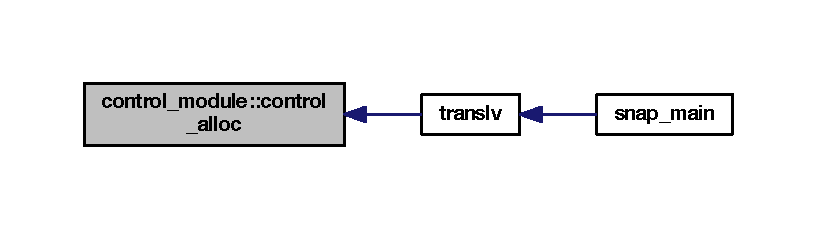
\includegraphics[width=350pt]{classcontrol__module_ac6bb07f4107c0d12f193aebfb73e233f_icgraph}
\end{center}
\end{figure}


\hypertarget{classcontrol__module_a2f968e7fae2c9dab97d81d4e8db154c8}{\index{control\-\_\-module@{control\-\_\-module}!control\-\_\-dealloc@{control\-\_\-dealloc}}
\index{control\-\_\-dealloc@{control\-\_\-dealloc}!control_module@{control\-\_\-module}}
\subsubsection[{control\-\_\-dealloc}]{\setlength{\rightskip}{0pt plus 5cm}subroutine control\-\_\-module\-::control\-\_\-dealloc (
\begin{DoxyParamCaption}
{}
\end{DoxyParamCaption}
)}}\label{classcontrol__module_a2f968e7fae2c9dab97d81d4e8db154c8}


Definition at line 96 of file control.\-f90.



Here is the caller graph for this function\-:\nopagebreak
\begin{figure}[H]
\begin{center}
\leavevmode
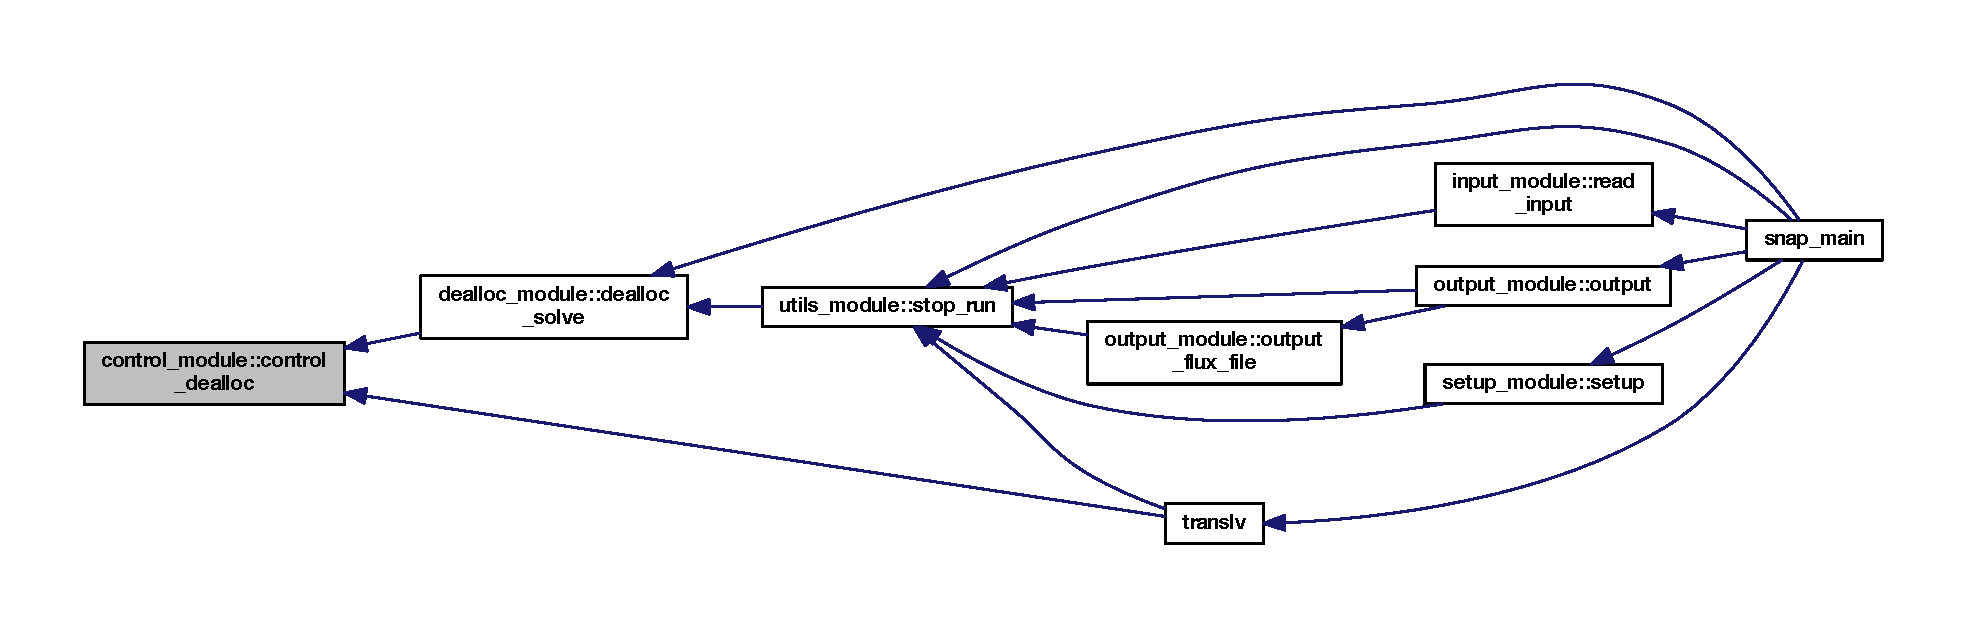
\includegraphics[width=350pt]{classcontrol__module_a2f968e7fae2c9dab97d81d4e8db154c8_icgraph}
\end{center}
\end{figure}




\subsection{Member Data Documentation}
\hypertarget{classcontrol__module_a39abfd20b09ff5ed5e22b69c92038156}{\index{control\-\_\-module@{control\-\_\-module}!dfmxi@{dfmxi}}
\index{dfmxi@{dfmxi}!control_module@{control\-\_\-module}}
\subsubsection[{dfmxi}]{\setlength{\rightskip}{0pt plus 5cm}real(r\-\_\-knd), dimension(\-:), allocatable control\-\_\-module\-::dfmxi}}\label{classcontrol__module_a39abfd20b09ff5ed5e22b69c92038156}


Definition at line 63 of file control.\-f90.

\hypertarget{classcontrol__module_a53a34dce98c72051d0043743774ea209}{\index{control\-\_\-module@{control\-\_\-module}!dfmxo@{dfmxo}}
\index{dfmxo@{dfmxo}!control_module@{control\-\_\-module}}
\subsubsection[{dfmxo}]{\setlength{\rightskip}{0pt plus 5cm}real(r\-\_\-knd) control\-\_\-module\-::dfmxo}}\label{classcontrol__module_a53a34dce98c72051d0043743774ea209}


Definition at line 59 of file control.\-f90.

\hypertarget{classcontrol__module_af466573cb3712b4a00c930a1720eeb68}{\index{control\-\_\-module@{control\-\_\-module}!dt@{dt}}
\index{dt@{dt}!control_module@{control\-\_\-module}}
\subsubsection[{dt}]{\setlength{\rightskip}{0pt plus 5cm}real(r\-\_\-knd) control\-\_\-module\-::dt}}\label{classcontrol__module_af466573cb3712b4a00c930a1720eeb68}


Definition at line 59 of file control.\-f90.

\hypertarget{classcontrol__module_af1c813926ca0adb64361e5b48a4f73b9}{\index{control\-\_\-module@{control\-\_\-module}!epsi@{epsi}}
\index{epsi@{epsi}!control_module@{control\-\_\-module}}
\subsubsection[{epsi}]{\setlength{\rightskip}{0pt plus 5cm}real(r\-\_\-knd) control\-\_\-module\-::epsi = 1.\-0\-E-\/4\-\_\-r\-\_\-knd}}\label{classcontrol__module_af1c813926ca0adb64361e5b48a4f73b9}


Definition at line 39 of file control.\-f90.

\hypertarget{classcontrol__module_ad305163b99235b021c5cf0f91e69c6d5}{\index{control\-\_\-module@{control\-\_\-module}!fixup@{fixup}}
\index{fixup@{fixup}!control_module@{control\-\_\-module}}
\subsubsection[{fixup}]{\setlength{\rightskip}{0pt plus 5cm}integer(i\-\_\-knd) control\-\_\-module\-::fixup = 0}}\label{classcontrol__module_ad305163b99235b021c5cf0f91e69c6d5}


Definition at line 36 of file control.\-f90.

\hypertarget{classcontrol__module_afb6375328be86057f0ac0af554c9abac}{\index{control\-\_\-module@{control\-\_\-module}!fluxp@{fluxp}}
\index{fluxp@{fluxp}!control_module@{control\-\_\-module}}
\subsubsection[{fluxp}]{\setlength{\rightskip}{0pt plus 5cm}integer(i\-\_\-knd) control\-\_\-module\-::fluxp = 0}}\label{classcontrol__module_afb6375328be86057f0ac0af554c9abac}


Definition at line 36 of file control.\-f90.

\hypertarget{classcontrol__module_a668776c82e56b5c08c95f01915287eb2}{\index{control\-\_\-module@{control\-\_\-module}!iitm@{iitm}}
\index{iitm@{iitm}!control_module@{control\-\_\-module}}
\subsubsection[{iitm}]{\setlength{\rightskip}{0pt plus 5cm}integer(i\-\_\-knd) control\-\_\-module\-::iitm = 5}}\label{classcontrol__module_a668776c82e56b5c08c95f01915287eb2}

\begin{DoxyParams}[1]{Parameters}
\mbox{\tt in}  & {\em epsi} & -\/ convergence criterion \\
\hline
\mbox{\tt in}  & {\em iitm} & -\/ max inner iterations \\
\hline
\end{DoxyParams}


Definition at line 36 of file control.\-f90.

\hypertarget{classcontrol__module_a800d3f9715c61376ad1a2d5b5b77e116}{\index{control\-\_\-module@{control\-\_\-module}!inrdone@{inrdone}}
\index{inrdone@{inrdone}!control_module@{control\-\_\-module}}
\subsubsection[{inrdone}]{\setlength{\rightskip}{0pt plus 5cm}logical(l\-\_\-knd), dimension(\-:), allocatable control\-\_\-module\-::inrdone}}\label{classcontrol__module_a800d3f9715c61376ad1a2d5b5b77e116}


Definition at line 57 of file control.\-f90.

\hypertarget{classcontrol__module_a47222ebdff0b8cbd932da30c43572177}{\index{control\-\_\-module@{control\-\_\-module}!it\-\_\-det@{it\-\_\-det}}
\index{it\-\_\-det@{it\-\_\-det}!control_module@{control\-\_\-module}}
\subsubsection[{it\-\_\-det}]{\setlength{\rightskip}{0pt plus 5cm}integer(i\-\_\-knd) control\-\_\-module\-::it\-\_\-det = 0}}\label{classcontrol__module_a47222ebdff0b8cbd932da30c43572177}


Definition at line 36 of file control.\-f90.

\hypertarget{classcontrol__module_a94e5569686ecc448c8fb807946cf95fb}{\index{control\-\_\-module@{control\-\_\-module}!nsteps@{nsteps}}
\index{nsteps@{nsteps}!control_module@{control\-\_\-module}}
\subsubsection[{nsteps}]{\setlength{\rightskip}{0pt plus 5cm}integer(i\-\_\-knd) control\-\_\-module\-::nsteps = 1}}\label{classcontrol__module_a94e5569686ecc448c8fb807946cf95fb}


Definition at line 36 of file control.\-f90.

\hypertarget{classcontrol__module_a99fddac51dc4299027ab5afd97c5c7ea}{\index{control\-\_\-module@{control\-\_\-module}!oitm@{oitm}}
\index{oitm@{oitm}!control_module@{control\-\_\-module}}
\subsubsection[{oitm}]{\setlength{\rightskip}{0pt plus 5cm}integer(i\-\_\-knd) control\-\_\-module\-::oitm = 100}}\label{classcontrol__module_a99fddac51dc4299027ab5afd97c5c7ea}


Definition at line 36 of file control.\-f90.

\hypertarget{classcontrol__module_a2a2bc582701b890779931ca8180a79e4}{\index{control\-\_\-module@{control\-\_\-module}!otrdone@{otrdone}}
\index{otrdone@{otrdone}!control_module@{control\-\_\-module}}
\subsubsection[{otrdone}]{\setlength{\rightskip}{0pt plus 5cm}logical(l\-\_\-knd) control\-\_\-module\-::otrdone}}\label{classcontrol__module_a2a2bc582701b890779931ca8180a79e4}


Definition at line 55 of file control.\-f90.

\hypertarget{classcontrol__module_a144620f0322c0ca01d9034fedd8d1076}{\index{control\-\_\-module@{control\-\_\-module}!tf@{tf}}
\index{tf@{tf}!control_module@{control\-\_\-module}}
\subsubsection[{tf}]{\setlength{\rightskip}{0pt plus 5cm}real(r\-\_\-knd) control\-\_\-module\-::tf = zero}}\label{classcontrol__module_a144620f0322c0ca01d9034fedd8d1076}


Definition at line 39 of file control.\-f90.

\hypertarget{classcontrol__module_a19077c84dfe2f11b40e39a9a63178731}{\index{control\-\_\-module@{control\-\_\-module}!timedep@{timedep}}
\index{timedep@{timedep}!control_module@{control\-\_\-module}}
\subsubsection[{timedep}]{\setlength{\rightskip}{0pt plus 5cm}integer(i\-\_\-knd) control\-\_\-module\-::timedep = 0}}\label{classcontrol__module_a19077c84dfe2f11b40e39a9a63178731}


Definition at line 36 of file control.\-f90.

\hypertarget{classcontrol__module_ad7c6872b7fb56bee7e7870e4ffa9dc65}{\index{control\-\_\-module@{control\-\_\-module}!tolr@{tolr}}
\index{tolr@{tolr}!control_module@{control\-\_\-module}}
\subsubsection[{tolr}]{\setlength{\rightskip}{0pt plus 5cm}real(r\-\_\-knd), parameter control\-\_\-module\-::tolr = 1.\-0\-E-\/12\-\_\-r\-\_\-knd}}\label{classcontrol__module_ad7c6872b7fb56bee7e7870e4ffa9dc65}


Definition at line 61 of file control.\-f90.



The documentation for this module was generated from the following file\-:\begin{DoxyCompactItemize}
\item 
src/\hyperlink{control_8f90}{control.\-f90}\end{DoxyCompactItemize}

\hypertarget{classdata__module}{\section{data\-\_\-module Module Reference}
\label{classdata__module}\index{data\-\_\-module@{data\-\_\-module}}
}


This module contains the variables and setup subroutines for the mock cross section data. It establishes the number of groups and constructs the cross section arrays.  


\subsection*{Public Member Functions}
\begin{DoxyCompactItemize}
\item 
subroutine \hyperlink{classdata__module_ade2204272a3d3184a17a625aec6795ab}{data\-\_\-allocate} (nx, ny, nz, nmom, nang, noct, timedep, istat)
\item 
subroutine \hyperlink{classdata__module_a64ba259f44e41619101dc90b61ef1b28}{data\-\_\-deallocate}
\end{DoxyCompactItemize}
\subsection*{Public Attributes}
\begin{DoxyCompactItemize}
\item 
integer(i\-\_\-knd) \hyperlink{classdata__module_a6ea7c9f76a6293c4f8b39b1782564561}{ng} = 1
\item 
integer(i\-\_\-knd) \hyperlink{classdata__module_a191b122ec7d6da5c691c45d89d65694f}{mat\-\_\-opt} = 0
\item 
integer(i\-\_\-knd) \hyperlink{classdata__module_aa630a65ce606a2869f55b214eeb6d9ec}{src\-\_\-opt} = 0
\item 
integer(i\-\_\-knd) \hyperlink{classdata__module_a7ac9af7f12e8f03d3ba40fa78904d5a1}{scatp} = 0
\item 
integer(i\-\_\-knd) \hyperlink{classdata__module_ad6de7dfbc5089cdc8cdfe59d6232f7d2}{nmat} = 1
\item 
integer(i\-\_\-knd), dimension(\-:,\-:,\-:), \\*
allocatable \hyperlink{classdata__module_aee30087acd108308e1a8e8bdd3f14dcf}{mat}
\item 
real(r\-\_\-knd), dimension(\-:), \\*
allocatable \hyperlink{classdata__module_a61d334d68509b4d5fac687707ac83241}{v}
\item 
real(r\-\_\-knd), dimension(\-:), \\*
allocatable \hyperlink{classdata__module_a8df0533fb95046e281a489f1c5dc9030}{vdelt}
\item 
real(r\-\_\-knd), dimension(\-:,\-:), \\*
allocatable \hyperlink{classdata__module_a3455329887f17be6b34eaa771348a3bf}{sigt}
\item 
real(r\-\_\-knd), dimension(\-:,\-:), \\*
allocatable \hyperlink{classdata__module_a536d3b44d8d6b245eabd2672f5cc8d65}{siga}
\item 
real(r\-\_\-knd), dimension(\-:,\-:), \\*
allocatable \hyperlink{classdata__module_a198158103501dbae827a7ccee2a1f91f}{sigs}
\item 
real(r\-\_\-knd), dimension(\-:,\-:,\-:,\-:), \\*
allocatable \hyperlink{classdata__module_a6d90b19307bcaef3132e6854534ba68f}{qi}
\item 
real(r\-\_\-knd), dimension(\-:,\-:,\-:,\-:), \\*
allocatable \hyperlink{classdata__module_a28dc2858f4b2054a06645430e7292d2a}{slgg}
\item 
real(r\-\_\-knd), dimension(\-:,\-:,\-:,\-:,\-:,\-:), \\*
allocatable \hyperlink{classdata__module_ab410d844881c0109e63b2e26e3dbbd37}{qim}
\end{DoxyCompactItemize}


\subsection{Detailed Description}
This module contains the variables and setup subroutines for the mock cross section data. It establishes the number of groups and constructs the cross section arrays. 

Definition at line 11 of file data.\-f90.



\subsection{Member Function/\-Subroutine Documentation}
\hypertarget{classdata__module_ade2204272a3d3184a17a625aec6795ab}{\index{data\-\_\-module@{data\-\_\-module}!data\-\_\-allocate@{data\-\_\-allocate}}
\index{data\-\_\-allocate@{data\-\_\-allocate}!data_module@{data\-\_\-module}}
\subsubsection[{data\-\_\-allocate}]{\setlength{\rightskip}{0pt plus 5cm}subroutine data\-\_\-module\-::data\-\_\-allocate (
\begin{DoxyParamCaption}
\item[{integer(i\-\_\-knd), intent(in)}]{nx, }
\item[{integer(i\-\_\-knd), intent(in)}]{ny, }
\item[{integer(i\-\_\-knd), intent(in)}]{nz, }
\item[{integer(i\-\_\-knd), intent(in)}]{nmom, }
\item[{integer(i\-\_\-knd), intent(in)}]{nang, }
\item[{integer(i\-\_\-knd), intent(in)}]{noct, }
\item[{integer(i\-\_\-knd), intent(in)}]{timedep, }
\item[{integer(i\-\_\-knd), intent(inout)}]{istat}
\end{DoxyParamCaption}
)}}\label{classdata__module_ade2204272a3d3184a17a625aec6795ab}


Definition at line 67 of file data.\-f90.



Here is the caller graph for this function\-:\nopagebreak
\begin{figure}[H]
\begin{center}
\leavevmode
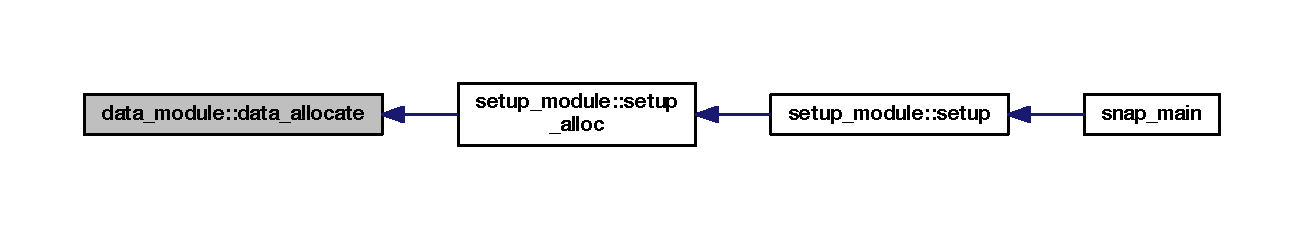
\includegraphics[width=350pt]{classdata__module_ade2204272a3d3184a17a625aec6795ab_icgraph}
\end{center}
\end{figure}


\hypertarget{classdata__module_a64ba259f44e41619101dc90b61ef1b28}{\index{data\-\_\-module@{data\-\_\-module}!data\-\_\-deallocate@{data\-\_\-deallocate}}
\index{data\-\_\-deallocate@{data\-\_\-deallocate}!data_module@{data\-\_\-module}}
\subsubsection[{data\-\_\-deallocate}]{\setlength{\rightskip}{0pt plus 5cm}subroutine data\-\_\-module\-::data\-\_\-deallocate (
\begin{DoxyParamCaption}
{}
\end{DoxyParamCaption}
)}}\label{classdata__module_a64ba259f44e41619101dc90b61ef1b28}


Definition at line 157 of file data.\-f90.



Here is the caller graph for this function\-:\nopagebreak
\begin{figure}[H]
\begin{center}
\leavevmode
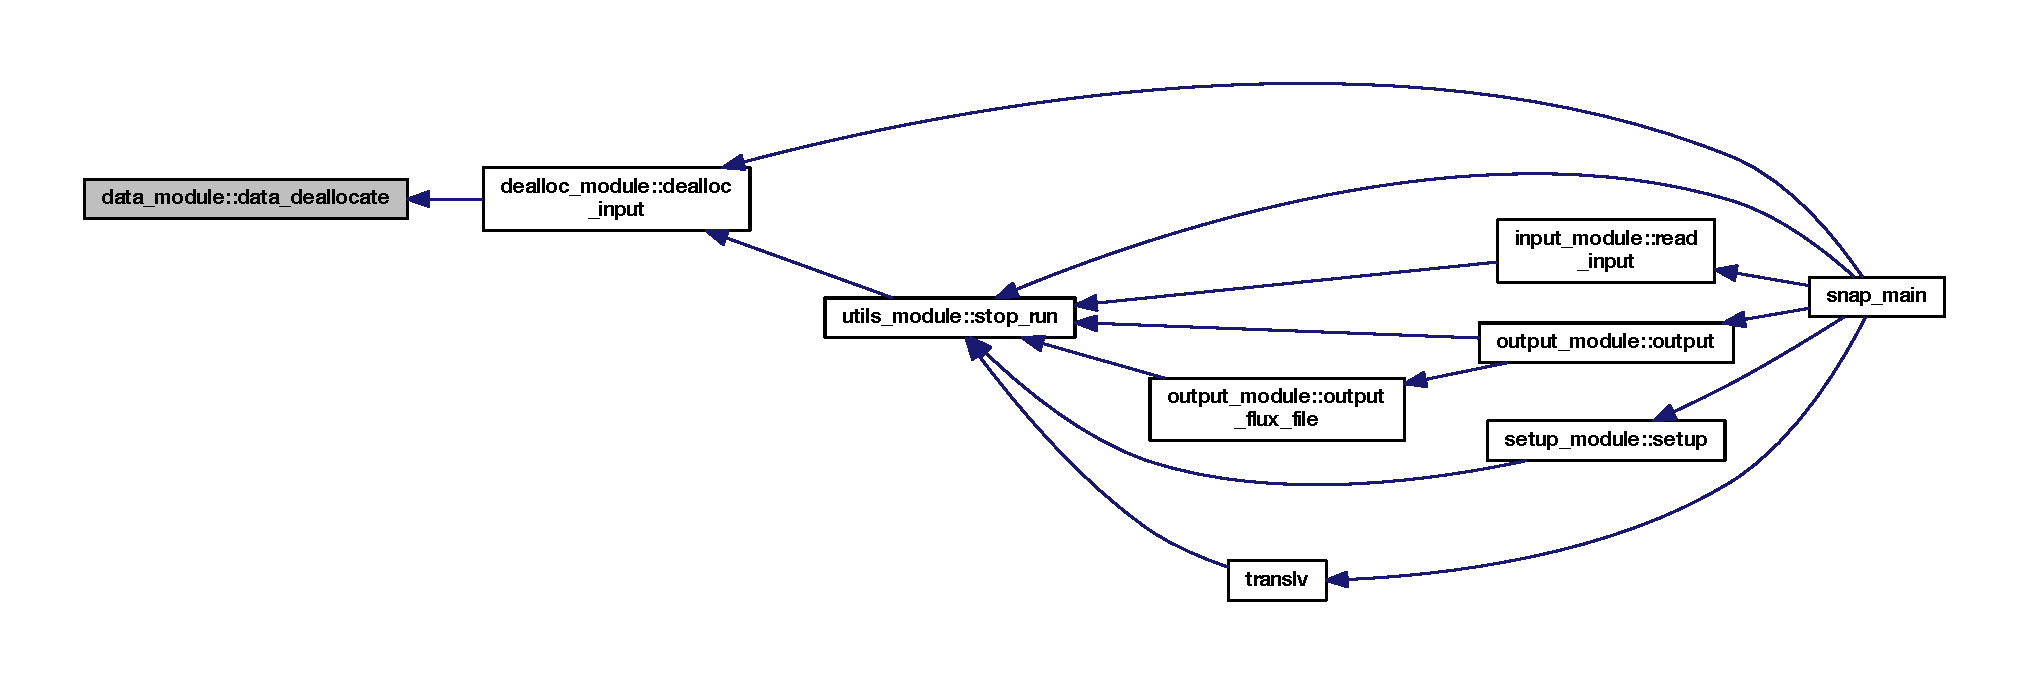
\includegraphics[width=350pt]{classdata__module_a64ba259f44e41619101dc90b61ef1b28_icgraph}
\end{center}
\end{figure}




\subsection{Member Data Documentation}
\hypertarget{classdata__module_aee30087acd108308e1a8e8bdd3f14dcf}{\index{data\-\_\-module@{data\-\_\-module}!mat@{mat}}
\index{mat@{mat}!data_module@{data\-\_\-module}}
\subsubsection[{mat}]{\setlength{\rightskip}{0pt plus 5cm}integer(i\-\_\-knd), dimension(\-:,\-:,\-:), allocatable data\-\_\-module\-::mat}}\label{classdata__module_aee30087acd108308e1a8e8bdd3f14dcf}


Definition at line 53 of file data.\-f90.

\hypertarget{classdata__module_a191b122ec7d6da5c691c45d89d65694f}{\index{data\-\_\-module@{data\-\_\-module}!mat\-\_\-opt@{mat\-\_\-opt}}
\index{mat\-\_\-opt@{mat\-\_\-opt}!data_module@{data\-\_\-module}}
\subsubsection[{mat\-\_\-opt}]{\setlength{\rightskip}{0pt plus 5cm}integer(i\-\_\-knd) data\-\_\-module\-::mat\-\_\-opt = 0}}\label{classdata__module_a191b122ec7d6da5c691c45d89d65694f}


Definition at line 32 of file data.\-f90.

\hypertarget{classdata__module_a6ea7c9f76a6293c4f8b39b1782564561}{\index{data\-\_\-module@{data\-\_\-module}!ng@{ng}}
\index{ng@{ng}!data_module@{data\-\_\-module}}
\subsubsection[{ng}]{\setlength{\rightskip}{0pt plus 5cm}integer(i\-\_\-knd) data\-\_\-module\-::ng = 1}}\label{classdata__module_a6ea7c9f76a6293c4f8b39b1782564561}


Definition at line 32 of file data.\-f90.

\hypertarget{classdata__module_ad6de7dfbc5089cdc8cdfe59d6232f7d2}{\index{data\-\_\-module@{data\-\_\-module}!nmat@{nmat}}
\index{nmat@{nmat}!data_module@{data\-\_\-module}}
\subsubsection[{nmat}]{\setlength{\rightskip}{0pt plus 5cm}integer(i\-\_\-knd) data\-\_\-module\-::nmat = 1}}\label{classdata__module_ad6de7dfbc5089cdc8cdfe59d6232f7d2}


Definition at line 51 of file data.\-f90.

\hypertarget{classdata__module_a6d90b19307bcaef3132e6854534ba68f}{\index{data\-\_\-module@{data\-\_\-module}!qi@{qi}}
\index{qi@{qi}!data_module@{data\-\_\-module}}
\subsubsection[{qi}]{\setlength{\rightskip}{0pt plus 5cm}real(r\-\_\-knd), dimension(\-:,\-:,\-:,\-:), allocatable data\-\_\-module\-::qi}}\label{classdata__module_a6d90b19307bcaef3132e6854534ba68f}


Definition at line 59 of file data.\-f90.

\hypertarget{classdata__module_ab410d844881c0109e63b2e26e3dbbd37}{\index{data\-\_\-module@{data\-\_\-module}!qim@{qim}}
\index{qim@{qim}!data_module@{data\-\_\-module}}
\subsubsection[{qim}]{\setlength{\rightskip}{0pt plus 5cm}real(r\-\_\-knd), dimension(\-:,\-:,\-:,\-:,\-:,\-:), allocatable data\-\_\-module\-::qim}}\label{classdata__module_ab410d844881c0109e63b2e26e3dbbd37}


Definition at line 61 of file data.\-f90.

\hypertarget{classdata__module_a7ac9af7f12e8f03d3ba40fa78904d5a1}{\index{data\-\_\-module@{data\-\_\-module}!scatp@{scatp}}
\index{scatp@{scatp}!data_module@{data\-\_\-module}}
\subsubsection[{scatp}]{\setlength{\rightskip}{0pt plus 5cm}integer(i\-\_\-knd) data\-\_\-module\-::scatp = 0}}\label{classdata__module_a7ac9af7f12e8f03d3ba40fa78904d5a1}


Definition at line 32 of file data.\-f90.

\hypertarget{classdata__module_a536d3b44d8d6b245eabd2672f5cc8d65}{\index{data\-\_\-module@{data\-\_\-module}!siga@{siga}}
\index{siga@{siga}!data_module@{data\-\_\-module}}
\subsubsection[{siga}]{\setlength{\rightskip}{0pt plus 5cm}real(r\-\_\-knd), dimension(\-:,\-:), allocatable data\-\_\-module\-::siga}}\label{classdata__module_a536d3b44d8d6b245eabd2672f5cc8d65}


Definition at line 57 of file data.\-f90.

\hypertarget{classdata__module_a198158103501dbae827a7ccee2a1f91f}{\index{data\-\_\-module@{data\-\_\-module}!sigs@{sigs}}
\index{sigs@{sigs}!data_module@{data\-\_\-module}}
\subsubsection[{sigs}]{\setlength{\rightskip}{0pt plus 5cm}real(r\-\_\-knd), dimension(\-:,\-:), allocatable data\-\_\-module\-::sigs}}\label{classdata__module_a198158103501dbae827a7ccee2a1f91f}


Definition at line 57 of file data.\-f90.

\hypertarget{classdata__module_a3455329887f17be6b34eaa771348a3bf}{\index{data\-\_\-module@{data\-\_\-module}!sigt@{sigt}}
\index{sigt@{sigt}!data_module@{data\-\_\-module}}
\subsubsection[{sigt}]{\setlength{\rightskip}{0pt plus 5cm}real(r\-\_\-knd), dimension(\-:,\-:), allocatable data\-\_\-module\-::sigt}}\label{classdata__module_a3455329887f17be6b34eaa771348a3bf}


Definition at line 57 of file data.\-f90.

\hypertarget{classdata__module_a28dc2858f4b2054a06645430e7292d2a}{\index{data\-\_\-module@{data\-\_\-module}!slgg@{slgg}}
\index{slgg@{slgg}!data_module@{data\-\_\-module}}
\subsubsection[{slgg}]{\setlength{\rightskip}{0pt plus 5cm}real(r\-\_\-knd), dimension(\-:,\-:,\-:,\-:), allocatable data\-\_\-module\-::slgg}}\label{classdata__module_a28dc2858f4b2054a06645430e7292d2a}


Definition at line 59 of file data.\-f90.

\hypertarget{classdata__module_aa630a65ce606a2869f55b214eeb6d9ec}{\index{data\-\_\-module@{data\-\_\-module}!src\-\_\-opt@{src\-\_\-opt}}
\index{src\-\_\-opt@{src\-\_\-opt}!data_module@{data\-\_\-module}}
\subsubsection[{src\-\_\-opt}]{\setlength{\rightskip}{0pt plus 5cm}integer(i\-\_\-knd) data\-\_\-module\-::src\-\_\-opt = 0}}\label{classdata__module_aa630a65ce606a2869f55b214eeb6d9ec}


Definition at line 32 of file data.\-f90.

\hypertarget{classdata__module_a61d334d68509b4d5fac687707ac83241}{\index{data\-\_\-module@{data\-\_\-module}!v@{v}}
\index{v@{v}!data_module@{data\-\_\-module}}
\subsubsection[{v}]{\setlength{\rightskip}{0pt plus 5cm}real(r\-\_\-knd), dimension(\-:), allocatable data\-\_\-module\-::v}}\label{classdata__module_a61d334d68509b4d5fac687707ac83241}


Definition at line 55 of file data.\-f90.

\hypertarget{classdata__module_a8df0533fb95046e281a489f1c5dc9030}{\index{data\-\_\-module@{data\-\_\-module}!vdelt@{vdelt}}
\index{vdelt@{vdelt}!data_module@{data\-\_\-module}}
\subsubsection[{vdelt}]{\setlength{\rightskip}{0pt plus 5cm}real(r\-\_\-knd), dimension(\-:), allocatable data\-\_\-module\-::vdelt}}\label{classdata__module_a8df0533fb95046e281a489f1c5dc9030}


Definition at line 55 of file data.\-f90.



The documentation for this module was generated from the following file\-:\begin{DoxyCompactItemize}
\item 
src/\hyperlink{data_8f90}{data.\-f90}\end{DoxyCompactItemize}

\hypertarget{classdealloc__module}{\section{dealloc\-\_\-module Module Reference}
\label{classdealloc__module}\index{dealloc\-\_\-module@{dealloc\-\_\-module}}
}
\subsection*{Public Member Functions}
\begin{DoxyCompactItemize}
\item 
subroutine \hyperlink{classdealloc__module_af080699b1fb3eca8000964ef28493a08}{dealloc\-\_\-input} (flg)
\item 
subroutine \hyperlink{classdealloc__module_ad1387c70d15b21e9b9595d3c2b7e85f6}{dealloc\-\_\-solve} (flg)
\end{DoxyCompactItemize}


\subsection{Detailed Description}


Definition at line 1 of file dealloc.\-f90.



\subsection{Member Function/\-Subroutine Documentation}
\hypertarget{classdealloc__module_af080699b1fb3eca8000964ef28493a08}{\index{dealloc\-\_\-module@{dealloc\-\_\-module}!dealloc\-\_\-input@{dealloc\-\_\-input}}
\index{dealloc\-\_\-input@{dealloc\-\_\-input}!dealloc_module@{dealloc\-\_\-module}}
\subsubsection[{dealloc\-\_\-input}]{\setlength{\rightskip}{0pt plus 5cm}subroutine dealloc\-\_\-module\-::dealloc\-\_\-input (
\begin{DoxyParamCaption}
\item[{integer(i\-\_\-knd), intent(in)}]{flg}
\end{DoxyParamCaption}
)}}\label{classdealloc__module_af080699b1fb3eca8000964ef28493a08}


Definition at line 31 of file dealloc.\-f90.



Here is the call graph for this function\-:\nopagebreak
\begin{figure}[H]
\begin{center}
\leavevmode
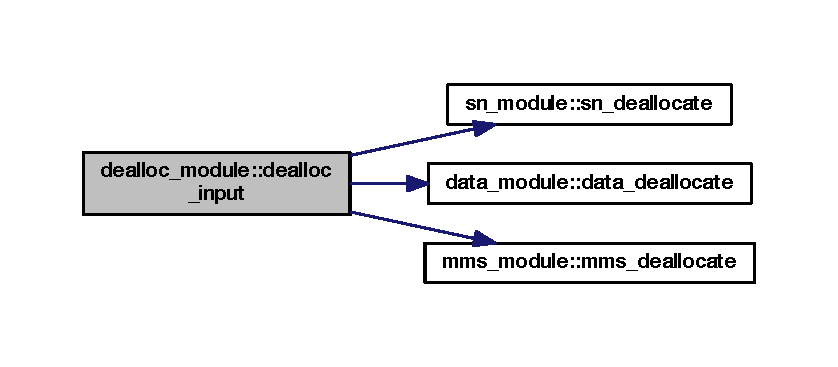
\includegraphics[width=350pt]{classdealloc__module_af080699b1fb3eca8000964ef28493a08_cgraph}
\end{center}
\end{figure}




Here is the caller graph for this function\-:\nopagebreak
\begin{figure}[H]
\begin{center}
\leavevmode
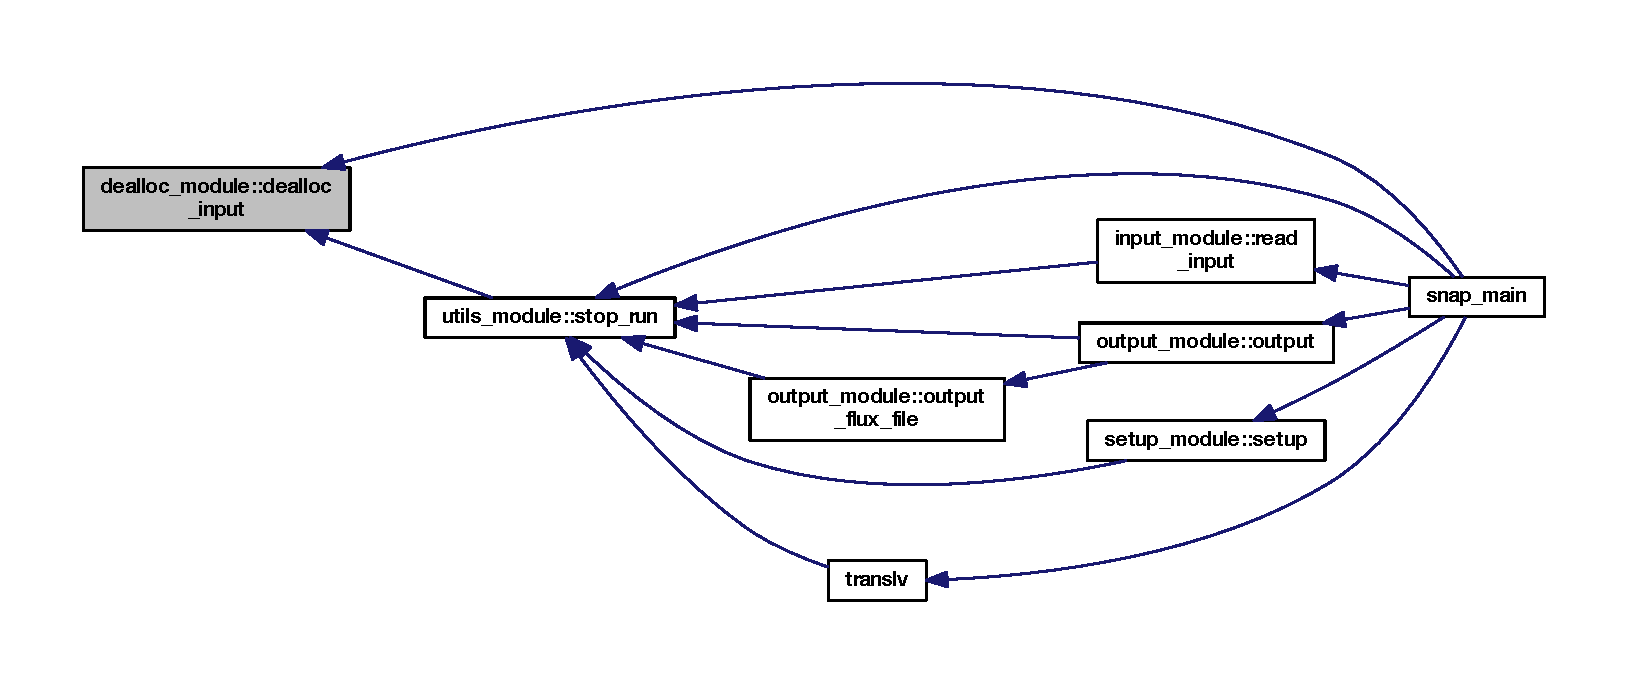
\includegraphics[width=350pt]{classdealloc__module_af080699b1fb3eca8000964ef28493a08_icgraph}
\end{center}
\end{figure}


\hypertarget{classdealloc__module_ad1387c70d15b21e9b9595d3c2b7e85f6}{\index{dealloc\-\_\-module@{dealloc\-\_\-module}!dealloc\-\_\-solve@{dealloc\-\_\-solve}}
\index{dealloc\-\_\-solve@{dealloc\-\_\-solve}!dealloc_module@{dealloc\-\_\-module}}
\subsubsection[{dealloc\-\_\-solve}]{\setlength{\rightskip}{0pt plus 5cm}subroutine dealloc\-\_\-module\-::dealloc\-\_\-solve (
\begin{DoxyParamCaption}
\item[{integer(i\-\_\-knd), intent(in)}]{flg}
\end{DoxyParamCaption}
)}}\label{classdealloc__module_ad1387c70d15b21e9b9595d3c2b7e85f6}


Definition at line 54 of file dealloc.\-f90.



Here is the call graph for this function\-:\nopagebreak
\begin{figure}[H]
\begin{center}
\leavevmode
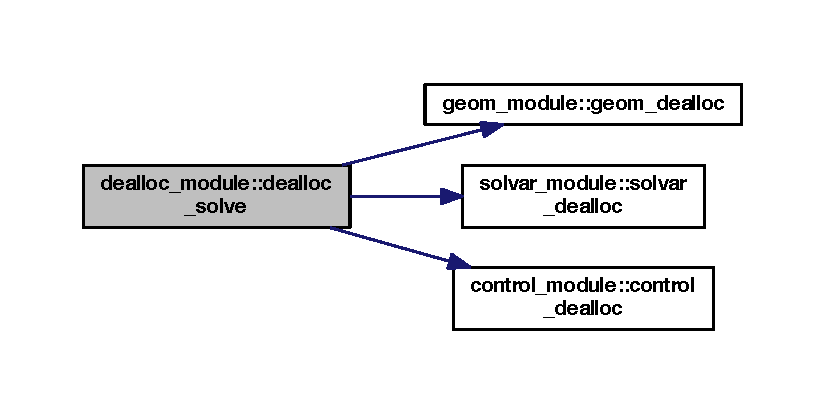
\includegraphics[width=350pt]{classdealloc__module_ad1387c70d15b21e9b9595d3c2b7e85f6_cgraph}
\end{center}
\end{figure}




Here is the caller graph for this function\-:\nopagebreak
\begin{figure}[H]
\begin{center}
\leavevmode
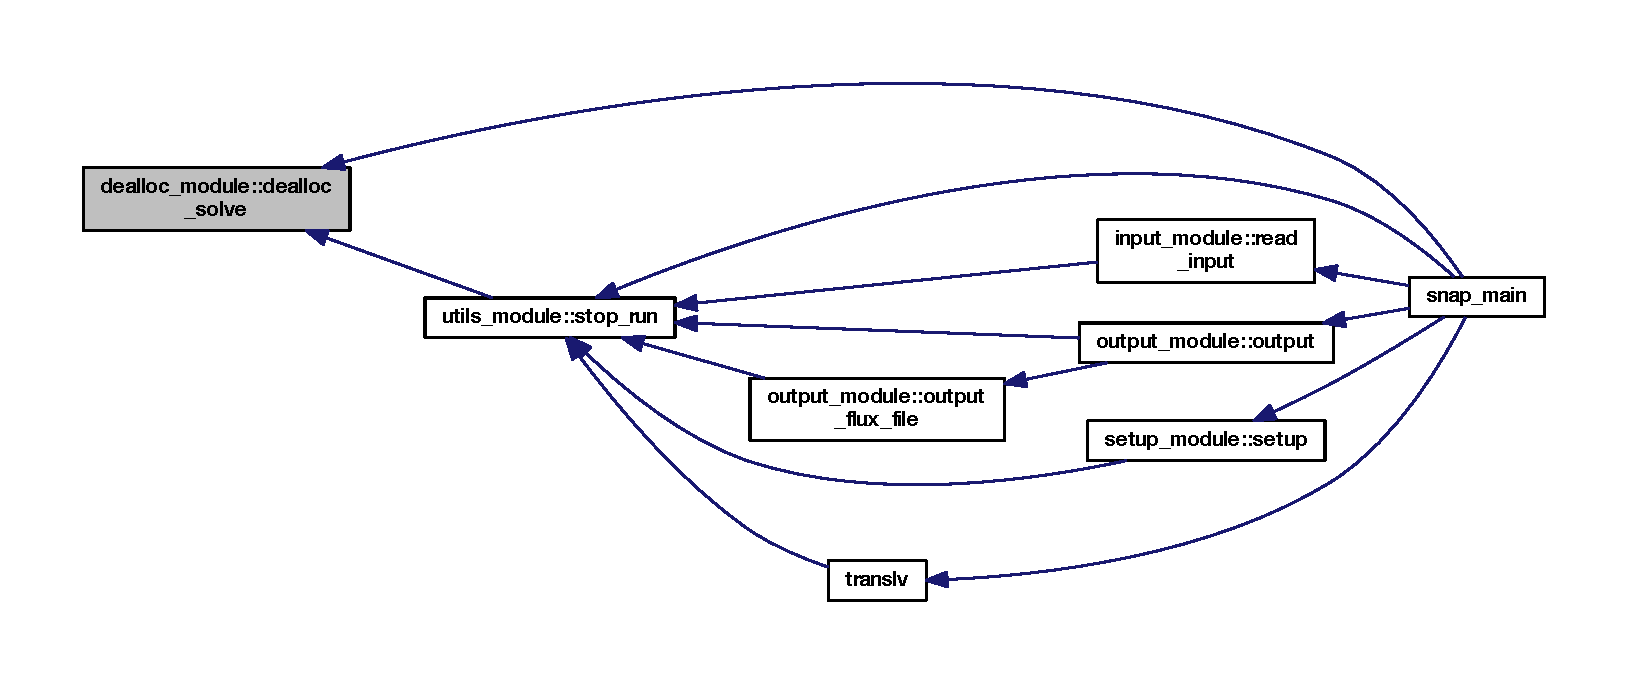
\includegraphics[width=350pt]{classdealloc__module_ad1387c70d15b21e9b9595d3c2b7e85f6_icgraph}
\end{center}
\end{figure}




The documentation for this module was generated from the following file\-:\begin{DoxyCompactItemize}
\item 
src/\hyperlink{dealloc_8f90}{dealloc.\-f90}\end{DoxyCompactItemize}

\hypertarget{classdim1__sweep__module}{\section{dim1\-\_\-sweep\-\_\-module Module Reference}
\label{classdim1__sweep__module}\index{dim1\-\_\-sweep\-\_\-module@{dim1\-\_\-sweep\-\_\-module}}
}
\subsection*{Public Member Functions}
\begin{DoxyCompactItemize}
\item 
subroutine, public \hyperlink{classdim1__sweep__module_aa0a270b2504bf7da636d3b3eaecdea16}{dim1\-\_\-sweep} (id, d1, d2, d3, d4, oct, g, psii, qtot, ec, vdelt, ptr\-\_\-in, ptr\-\_\-out, dinv, flux, fluxm, wmu, flkx, t\-\_\-xs)
\end{DoxyCompactItemize}
\subsection*{Public Attributes}
\begin{DoxyCompactItemize}
\item 
real(r\-\_\-knd) \hyperlink{classdim1__sweep__module_a9b0ce6702181b5c9bf98ac179929a1aa}{fmin} = zero
\item 
real(r\-\_\-knd) \hyperlink{classdim1__sweep__module_a973f03dda9d8fe7662d437c0c790f3a2}{fmax} = zero
\end{DoxyCompactItemize}


\subsection{Detailed Description}


Definition at line 1 of file dim1\-\_\-sweep.\-f90.



\subsection{Member Function/\-Subroutine Documentation}
\hypertarget{classdim1__sweep__module_aa0a270b2504bf7da636d3b3eaecdea16}{\index{dim1\-\_\-sweep\-\_\-module@{dim1\-\_\-sweep\-\_\-module}!dim1\-\_\-sweep@{dim1\-\_\-sweep}}
\index{dim1\-\_\-sweep@{dim1\-\_\-sweep}!dim1_sweep_module@{dim1\-\_\-sweep\-\_\-module}}
\subsubsection[{dim1\-\_\-sweep}]{\setlength{\rightskip}{0pt plus 5cm}subroutine, public dim1\-\_\-sweep\-\_\-module\-::dim1\-\_\-sweep (
\begin{DoxyParamCaption}
\item[{integer(i\-\_\-knd), intent(in)}]{id, }
\item[{integer(i\-\_\-knd), intent(in)}]{d1, }
\item[{integer(i\-\_\-knd), intent(in)}]{d2, }
\item[{integer(i\-\_\-knd), intent(in)}]{d3, }
\item[{integer(i\-\_\-knd), intent(in)}]{d4, }
\item[{integer(i\-\_\-knd), intent(in)}]{oct, }
\item[{integer(i\-\_\-knd), intent(in)}]{g, }
\item[{real(r\-\_\-knd), dimension(nang), intent(inout)}]{psii, }
\item[{real(r\-\_\-knd), dimension(cmom,nx), intent(in)}]{qtot, }
\item[{real(r\-\_\-knd), dimension(nang,cmom), intent(in)}]{ec, }
\item[{real(r\-\_\-knd), intent(in)}]{vdelt, }
\item[{real(r\-\_\-knd), dimension(d1,d2,d3,d4), intent(in)}]{ptr\-\_\-in, }
\item[{real(r\-\_\-knd), dimension(d1,d2,d3,d4), intent(out)}]{ptr\-\_\-out, }
\item[{real(r\-\_\-knd), dimension(nang,nx), intent(in)}]{dinv, }
\item[{real(r\-\_\-knd), dimension(nx), intent(inout)}]{flux, }
\item[{real(r\-\_\-knd), dimension(cmom-\/1,nx), intent(inout)}]{fluxm, }
\item[{real(r\-\_\-knd), dimension(nang), intent(in)}]{wmu, }
\item[{real(r\-\_\-knd), dimension(nx), intent(inout)}]{flkx, }
\item[{real(r\-\_\-knd), dimension(nx), intent(in)}]{t\-\_\-xs}
\end{DoxyParamCaption}
)}}\label{classdim1__sweep__module_aa0a270b2504bf7da636d3b3eaecdea16}


Definition at line 39 of file dim1\-\_\-sweep.\-f90.



Here is the caller graph for this function\-:\nopagebreak
\begin{figure}[H]
\begin{center}
\leavevmode
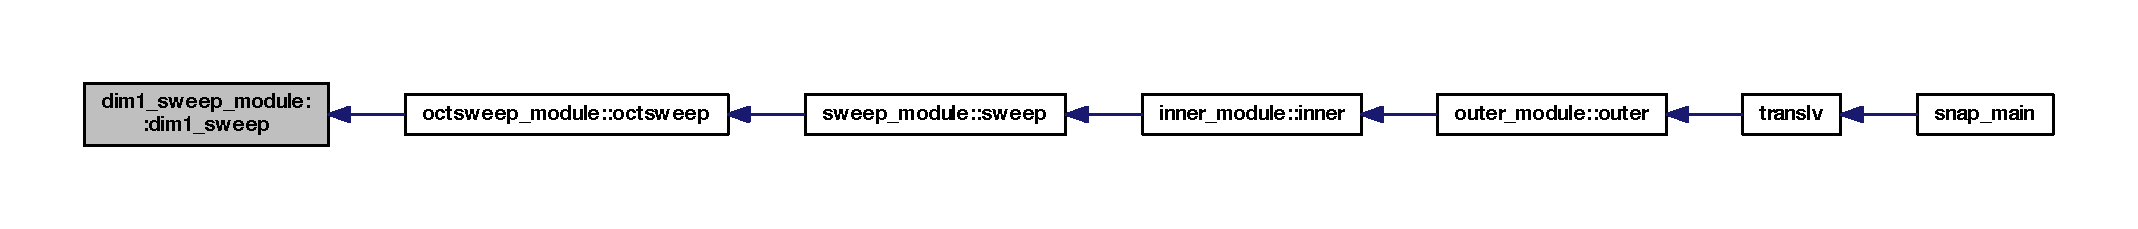
\includegraphics[width=350pt]{classdim1__sweep__module_aa0a270b2504bf7da636d3b3eaecdea16_icgraph}
\end{center}
\end{figure}




\subsection{Member Data Documentation}
\hypertarget{classdim1__sweep__module_a973f03dda9d8fe7662d437c0c790f3a2}{\index{dim1\-\_\-sweep\-\_\-module@{dim1\-\_\-sweep\-\_\-module}!fmax@{fmax}}
\index{fmax@{fmax}!dim1_sweep_module@{dim1\-\_\-sweep\-\_\-module}}
\subsubsection[{fmax}]{\setlength{\rightskip}{0pt plus 5cm}real(r\-\_\-knd) dim1\-\_\-sweep\-\_\-module\-::fmax = zero}}\label{classdim1__sweep__module_a973f03dda9d8fe7662d437c0c790f3a2}


Definition at line 33 of file dim1\-\_\-sweep.\-f90.

\hypertarget{classdim1__sweep__module_a9b0ce6702181b5c9bf98ac179929a1aa}{\index{dim1\-\_\-sweep\-\_\-module@{dim1\-\_\-sweep\-\_\-module}!fmin@{fmin}}
\index{fmin@{fmin}!dim1_sweep_module@{dim1\-\_\-sweep\-\_\-module}}
\subsubsection[{fmin}]{\setlength{\rightskip}{0pt plus 5cm}real(r\-\_\-knd) dim1\-\_\-sweep\-\_\-module\-::fmin = zero}}\label{classdim1__sweep__module_a9b0ce6702181b5c9bf98ac179929a1aa}


Definition at line 33 of file dim1\-\_\-sweep.\-f90.



The documentation for this module was generated from the following file\-:\begin{DoxyCompactItemize}
\item 
src/\hyperlink{dim1__sweep_8f90}{dim1\-\_\-sweep.\-f90}\end{DoxyCompactItemize}

\hypertarget{classdim3__sweep__module}{\section{dim3\-\_\-sweep\-\_\-module Module Reference}
\label{classdim3__sweep__module}\index{dim3\-\_\-sweep\-\_\-module@{dim3\-\_\-sweep\-\_\-module}}
}


This module contains the 2\-D and 3\-D mesh sweep logic.  


\subsection*{Public Member Functions}
\begin{DoxyCompactItemize}
\item 
subroutine, public \hyperlink{classdim3__sweep__module_a201ea00518f54fac4152d4ce277de50d}{dim3\-\_\-sweep} (ich, id, d1, d2, d3, d4, jd, kd, jlo, klo, oct, g, jhi, khi, jst, kst, psii, psij, psik, qtot, ec, vdelt, ptr\-\_\-in, ptr\-\_\-out, dinv, flux, fluxm, jb\-\_\-in, jb\-\_\-out, kb\-\_\-in, kb\-\_\-out, wmu, weta, wxi, flkx, flky, flkz, t\-\_\-xs)
\end{DoxyCompactItemize}
\subsection*{Public Attributes}
\begin{DoxyCompactItemize}
\item 
real(r\-\_\-knd) \hyperlink{classdim3__sweep__module_a5ec448e8a99070a51d62e75a430a9c60}{fmin} = zero
\item 
real(r\-\_\-knd) \hyperlink{classdim3__sweep__module_aac295110595a9c85602d58906d51cd46}{fmax} = zero
\end{DoxyCompactItemize}


\subsection{Detailed Description}
This module contains the 2\-D and 3\-D mesh sweep logic. 

Definition at line 9 of file dim3\-\_\-sweep.\-f90.



\subsection{Member Function/\-Subroutine Documentation}
\hypertarget{classdim3__sweep__module_a201ea00518f54fac4152d4ce277de50d}{\index{dim3\-\_\-sweep\-\_\-module@{dim3\-\_\-sweep\-\_\-module}!dim3\-\_\-sweep@{dim3\-\_\-sweep}}
\index{dim3\-\_\-sweep@{dim3\-\_\-sweep}!dim3_sweep_module@{dim3\-\_\-sweep\-\_\-module}}
\subsubsection[{dim3\-\_\-sweep}]{\setlength{\rightskip}{0pt plus 5cm}subroutine, public dim3\-\_\-sweep\-\_\-module\-::dim3\-\_\-sweep (
\begin{DoxyParamCaption}
\item[{integer(i\-\_\-knd), intent(in)}]{ich, }
\item[{integer(i\-\_\-knd), intent(in)}]{id, }
\item[{integer(i\-\_\-knd), intent(in)}]{d1, }
\item[{integer(i\-\_\-knd), intent(in)}]{d2, }
\item[{integer(i\-\_\-knd), intent(in)}]{d3, }
\item[{integer(i\-\_\-knd), intent(in)}]{d4, }
\item[{integer(i\-\_\-knd), intent(in)}]{jd, }
\item[{integer(i\-\_\-knd), intent(in)}]{kd, }
\item[{integer(i\-\_\-knd), intent(in)}]{jlo, }
\item[{integer(i\-\_\-knd), intent(in)}]{klo, }
\item[{integer(i\-\_\-knd), intent(in)}]{oct, }
\item[{integer(i\-\_\-knd), intent(in)}]{g, }
\item[{integer(i\-\_\-knd), intent(in)}]{jhi, }
\item[{integer(i\-\_\-knd), intent(in)}]{khi, }
\item[{integer(i\-\_\-knd), intent(in)}]{jst, }
\item[{integer(i\-\_\-knd), intent(in)}]{kst, }
\item[{real(r\-\_\-knd), dimension(nang,ny,nz), intent(inout)}]{psii, }
\item[{real(r\-\_\-knd), dimension(nang,ichunk), intent(inout)}]{psij, }
\item[{real(r\-\_\-knd), dimension(nang,ichunk,ny), intent(inout)}]{psik, }
\item[{real(r\-\_\-knd), dimension(cmom,nx,ny,nz), intent(in)}]{qtot, }
\item[{real(r\-\_\-knd), dimension(nang,cmom), intent(in)}]{ec, }
\item[{real(r\-\_\-knd), intent(in)}]{vdelt, }
\item[{real(r\-\_\-knd), dimension(d1,d2,d3,d4), intent(in)}]{ptr\-\_\-in, }
\item[{real(r\-\_\-knd), dimension(d1,d2,d3,d4), intent(out)}]{ptr\-\_\-out, }
\item[{real(r\-\_\-knd), dimension(nang,nx,ny,nz), intent(in)}]{dinv, }
\item[{real(r\-\_\-knd), dimension(nx,ny,nz), intent(inout)}]{flux, }
\item[{real(r\-\_\-knd), dimension(cmom-\/1,nx,ny,nz), intent(inout)}]{fluxm, }
\item[{real(r\-\_\-knd), dimension(nang,ichunk,nz), intent(in)}]{jb\-\_\-in, }
\item[{real(r\-\_\-knd), dimension(nang,ichunk,nz), intent(out)}]{jb\-\_\-out, }
\item[{real(r\-\_\-knd), dimension(nang,ichunk,ny), intent(in)}]{kb\-\_\-in, }
\item[{real(r\-\_\-knd), dimension(nang,ichunk,ny), intent(out)}]{kb\-\_\-out, }
\item[{real(r\-\_\-knd), dimension(nang), intent(in)}]{wmu, }
\item[{real(r\-\_\-knd), dimension(nang), intent(in)}]{weta, }
\item[{real(r\-\_\-knd), dimension(nang), intent(in)}]{wxi, }
\item[{real(r\-\_\-knd), dimension(nx+1,ny,nz), intent(inout)}]{flkx, }
\item[{real(r\-\_\-knd), dimension(nx,ny+1,nz), intent(inout)}]{flky, }
\item[{real(r\-\_\-knd), dimension(nx,ny,nz+1), intent(inout)}]{flkz, }
\item[{real(r\-\_\-knd), dimension(nx,ny,nz), intent(in)}]{t\-\_\-xs}
\end{DoxyParamCaption}
)}}\label{classdim3__sweep__module_a201ea00518f54fac4152d4ce277de50d}


Definition at line 43 of file dim3\-\_\-sweep.\-f90.



Here is the caller graph for this function\-:\nopagebreak
\begin{figure}[H]
\begin{center}
\leavevmode
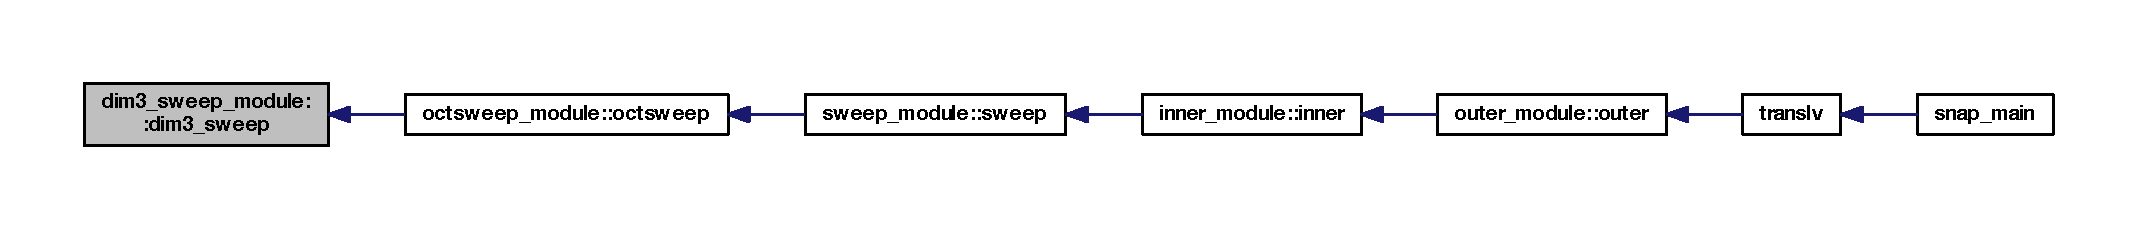
\includegraphics[width=350pt]{classdim3__sweep__module_a201ea00518f54fac4152d4ce277de50d_icgraph}
\end{center}
\end{figure}




\subsection{Member Data Documentation}
\hypertarget{classdim3__sweep__module_aac295110595a9c85602d58906d51cd46}{\index{dim3\-\_\-sweep\-\_\-module@{dim3\-\_\-sweep\-\_\-module}!fmax@{fmax}}
\index{fmax@{fmax}!dim3_sweep_module@{dim3\-\_\-sweep\-\_\-module}}
\subsubsection[{fmax}]{\setlength{\rightskip}{0pt plus 5cm}real(r\-\_\-knd) dim3\-\_\-sweep\-\_\-module\-::fmax = zero}}\label{classdim3__sweep__module_aac295110595a9c85602d58906d51cd46}


Definition at line 37 of file dim3\-\_\-sweep.\-f90.

\hypertarget{classdim3__sweep__module_a5ec448e8a99070a51d62e75a430a9c60}{\index{dim3\-\_\-sweep\-\_\-module@{dim3\-\_\-sweep\-\_\-module}!fmin@{fmin}}
\index{fmin@{fmin}!dim3_sweep_module@{dim3\-\_\-sweep\-\_\-module}}
\subsubsection[{fmin}]{\setlength{\rightskip}{0pt plus 5cm}real(r\-\_\-knd) dim3\-\_\-sweep\-\_\-module\-::fmin = zero}}\label{classdim3__sweep__module_a5ec448e8a99070a51d62e75a430a9c60}


Definition at line 37 of file dim3\-\_\-sweep.\-f90.



The documentation for this module was generated from the following file\-:\begin{DoxyCompactItemize}
\item 
src/\hyperlink{dim3__sweep_8f90}{dim3\-\_\-sweep.\-f90}\end{DoxyCompactItemize}

\hypertarget{classexpxs__module}{\section{expxs\-\_\-module Module Reference}
\label{classexpxs__module}\index{expxs\-\_\-module@{expxs\-\_\-module}}
}
\subsection*{Public Member Functions}
\begin{DoxyCompactItemize}
\item 
subroutine \hyperlink{classexpxs__module_a1360b06c8a60da7064b478a1103dff99}{expxs\-\_\-reg} (xs, map, cs)
\item 
subroutine \hyperlink{classexpxs__module_a4ae798f15df616045ca167c04d5b564e}{expxs\-\_\-slgg} (scat, map, cs)
\end{DoxyCompactItemize}


\subsection{Detailed Description}


Definition at line 1 of file expxs.\-f90.



\subsection{Member Function/\-Subroutine Documentation}
\hypertarget{classexpxs__module_a1360b06c8a60da7064b478a1103dff99}{\index{expxs\-\_\-module@{expxs\-\_\-module}!expxs\-\_\-reg@{expxs\-\_\-reg}}
\index{expxs\-\_\-reg@{expxs\-\_\-reg}!expxs_module@{expxs\-\_\-module}}
\subsubsection[{expxs\-\_\-reg}]{\setlength{\rightskip}{0pt plus 5cm}subroutine expxs\-\_\-module\-::expxs\-\_\-reg (
\begin{DoxyParamCaption}
\item[{real(r\-\_\-knd), dimension(nmat), intent(in)}]{xs, }
\item[{integer(i\-\_\-knd), dimension(nx,ny,nz), intent(in)}]{map, }
\item[{real(r\-\_\-knd), dimension(nx,ny,nz), intent(out)}]{cs}
\end{DoxyParamCaption}
)}}\label{classexpxs__module_a1360b06c8a60da7064b478a1103dff99}


Definition at line 28 of file expxs.\-f90.



Here is the caller graph for this function\-:\nopagebreak
\begin{figure}[H]
\begin{center}
\leavevmode
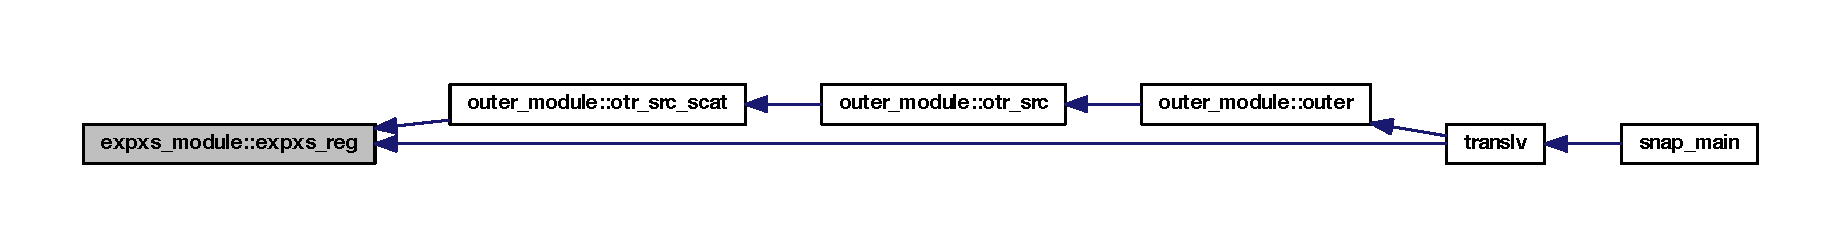
\includegraphics[width=350pt]{classexpxs__module_a1360b06c8a60da7064b478a1103dff99_icgraph}
\end{center}
\end{figure}


\hypertarget{classexpxs__module_a4ae798f15df616045ca167c04d5b564e}{\index{expxs\-\_\-module@{expxs\-\_\-module}!expxs\-\_\-slgg@{expxs\-\_\-slgg}}
\index{expxs\-\_\-slgg@{expxs\-\_\-slgg}!expxs_module@{expxs\-\_\-module}}
\subsubsection[{expxs\-\_\-slgg}]{\setlength{\rightskip}{0pt plus 5cm}subroutine expxs\-\_\-module\-::expxs\-\_\-slgg (
\begin{DoxyParamCaption}
\item[{real(r\-\_\-knd), dimension(nmat,nmom), intent(in)}]{scat, }
\item[{integer(i\-\_\-knd), dimension(nx,ny,nz), intent(in)}]{map, }
\item[{real(r\-\_\-knd), dimension(nmom,nx,ny,nz), intent(out)}]{cs}
\end{DoxyParamCaption}
)}}\label{classexpxs__module_a4ae798f15df616045ca167c04d5b564e}


Definition at line 66 of file expxs.\-f90.



Here is the caller graph for this function\-:\nopagebreak
\begin{figure}[H]
\begin{center}
\leavevmode
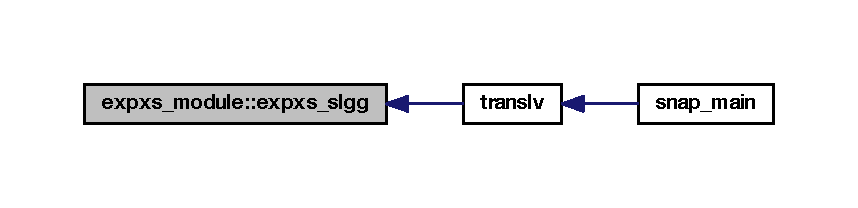
\includegraphics[width=350pt]{classexpxs__module_a4ae798f15df616045ca167c04d5b564e_icgraph}
\end{center}
\end{figure}




The documentation for this module was generated from the following file\-:\begin{DoxyCompactItemize}
\item 
src/\hyperlink{expxs_8f90}{expxs.\-f90}\end{DoxyCompactItemize}

\hypertarget{classgeom__module}{\section{geom\-\_\-module Module Reference}
\label{classgeom__module}\index{geom\-\_\-module@{geom\-\_\-module}}
}


This module contains the variables that relate to the geometry of the problem and the subroutines necessary to allocate and deallocate geometry related data as necessary.  


\subsection*{Public Member Functions}
\begin{DoxyCompactItemize}
\item 
subroutine \hyperlink{classgeom__module_ac4ae76d14c7253c3c87ae0f55b1d4b1a}{geom\-\_\-alloc} (nang, ng, ierr)
\item 
subroutine \hyperlink{classgeom__module_ab2401a2eca471da4ca28fe634b5350d4}{geom\-\_\-dealloc}
\item 
subroutine \hyperlink{classgeom__module_aa09319572e809c686211758ef5fb129e}{param\-\_\-calc} (ichunk, nang, mu, eta, xi, cs, vd, d)
\end{DoxyCompactItemize}
\subsection*{Public Attributes}
\begin{DoxyCompactItemize}
\item 
integer(i\-\_\-knd) \hyperlink{classgeom__module_a764bf4ab4dc187512c803d73505e6b57}{ndimen} = 1
\item 
integer(i\-\_\-knd) \hyperlink{classgeom__module_a7a5902416f1d33e2a27620d6c82db061}{nx} = 4
\item 
integer(i\-\_\-knd) \hyperlink{classgeom__module_a38b87580d41ec11b8719f65f06b8b0a3}{ny} = 1
\item 
integer(i\-\_\-knd) \hyperlink{classgeom__module_a5f461a2f10c78de302a44c8c70b8fca5}{nz} = 1
\item 
real(r\-\_\-knd) \hyperlink{classgeom__module_a1fe9e4dc8297fc98198b561000a97973}{lx} = one
\item 
real(r\-\_\-knd) \hyperlink{classgeom__module_adc5d5005b562bb94578c33b5bcde0012}{ly} = one
\item 
real(r\-\_\-knd) \hyperlink{classgeom__module_aba080d6dd2b57ad40676a7331daaa824}{lz} = one
\item 
integer(i\-\_\-knd) \hyperlink{classgeom__module_a28abec0d4fe709bc64ee36b68347ce1a}{ny\-\_\-gl}
\item 
integer(i\-\_\-knd) \hyperlink{classgeom__module_a3d237cf21a21064504566ce34b27c848}{nz\-\_\-gl}
\item 
integer(i\-\_\-knd) \hyperlink{classgeom__module_a87c8f8859d2d98c1dfc36f0ccf4208df}{jlb}
\item 
integer(i\-\_\-knd) \hyperlink{classgeom__module_ada7a9e753e21b30a06f0858f5deb4300}{jub}
\item 
integer(i\-\_\-knd) \hyperlink{classgeom__module_a7c3abb8b57ed30570288a1da71db8444}{klb}
\item 
integer(i\-\_\-knd) \hyperlink{classgeom__module_a79842b1abc678e999d926bc361620371}{kub}
\item 
integer(i\-\_\-knd) \hyperlink{classgeom__module_af92dc09eacd9c240bd51ea2792a13820}{nc}
\item 
real(r\-\_\-knd) \hyperlink{classgeom__module_a2f292c19b0e9bfc4cde1d54f0e9d4472}{dx}
\item 
real(r\-\_\-knd) \hyperlink{classgeom__module_a13234163c83c1041d8053ab0f4ea5d40}{dy}
\item 
real(r\-\_\-knd) \hyperlink{classgeom__module_a59842db695f66127f749bffd9df2f034}{dz}
\item 
real(r\-\_\-knd) \hyperlink{classgeom__module_af657687714307a2bfe5e99ea8ee9f35e}{hi}
\item 
real(r\-\_\-knd), dimension(\-:), \\*
allocatable \hyperlink{classgeom__module_ad5db4c62807a7025e92dd2c5742156eb}{hj}
\item 
real(r\-\_\-knd), dimension(\-:), \\*
allocatable \hyperlink{classgeom__module_a42bd1a5bffae9b223ac63ce018664023}{hk}
\item 
real(r\-\_\-knd), dimension(\-:,\-:,\-:,\-:,\-:), \\*
allocatable \hyperlink{classgeom__module_ae4c351982371a6870429ab660ec35e45}{dinv}
\end{DoxyCompactItemize}


\subsection{Detailed Description}
This module contains the variables that relate to the geometry of the problem and the subroutines necessary to allocate and deallocate geometry related data as necessary. 

Definition at line 11 of file geom.\-f90.



\subsection{Member Function/\-Subroutine Documentation}
\hypertarget{classgeom__module_ac4ae76d14c7253c3c87ae0f55b1d4b1a}{\index{geom\-\_\-module@{geom\-\_\-module}!geom\-\_\-alloc@{geom\-\_\-alloc}}
\index{geom\-\_\-alloc@{geom\-\_\-alloc}!geom_module@{geom\-\_\-module}}
\subsubsection[{geom\-\_\-alloc}]{\setlength{\rightskip}{0pt plus 5cm}subroutine geom\-\_\-module\-::geom\-\_\-alloc (
\begin{DoxyParamCaption}
\item[{integer(i\-\_\-knd), intent(in)}]{nang, }
\item[{integer(i\-\_\-knd), intent(in)}]{ng, }
\item[{integer(i\-\_\-knd), intent(out)}]{ierr}
\end{DoxyParamCaption}
)}}\label{classgeom__module_ac4ae76d14c7253c3c87ae0f55b1d4b1a}


Definition at line 74 of file geom.\-f90.



Here is the caller graph for this function\-:\nopagebreak
\begin{figure}[H]
\begin{center}
\leavevmode
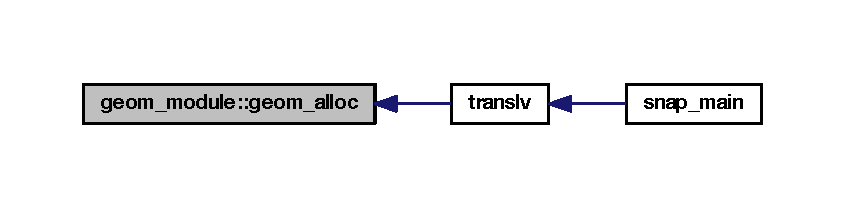
\includegraphics[width=350pt]{classgeom__module_ac4ae76d14c7253c3c87ae0f55b1d4b1a_icgraph}
\end{center}
\end{figure}


\hypertarget{classgeom__module_ab2401a2eca471da4ca28fe634b5350d4}{\index{geom\-\_\-module@{geom\-\_\-module}!geom\-\_\-dealloc@{geom\-\_\-dealloc}}
\index{geom\-\_\-dealloc@{geom\-\_\-dealloc}!geom_module@{geom\-\_\-module}}
\subsubsection[{geom\-\_\-dealloc}]{\setlength{\rightskip}{0pt plus 5cm}subroutine geom\-\_\-module\-::geom\-\_\-dealloc (
\begin{DoxyParamCaption}
{}
\end{DoxyParamCaption}
)}}\label{classgeom__module_ab2401a2eca471da4ca28fe634b5350d4}


Definition at line 102 of file geom.\-f90.



Here is the caller graph for this function\-:\nopagebreak
\begin{figure}[H]
\begin{center}
\leavevmode
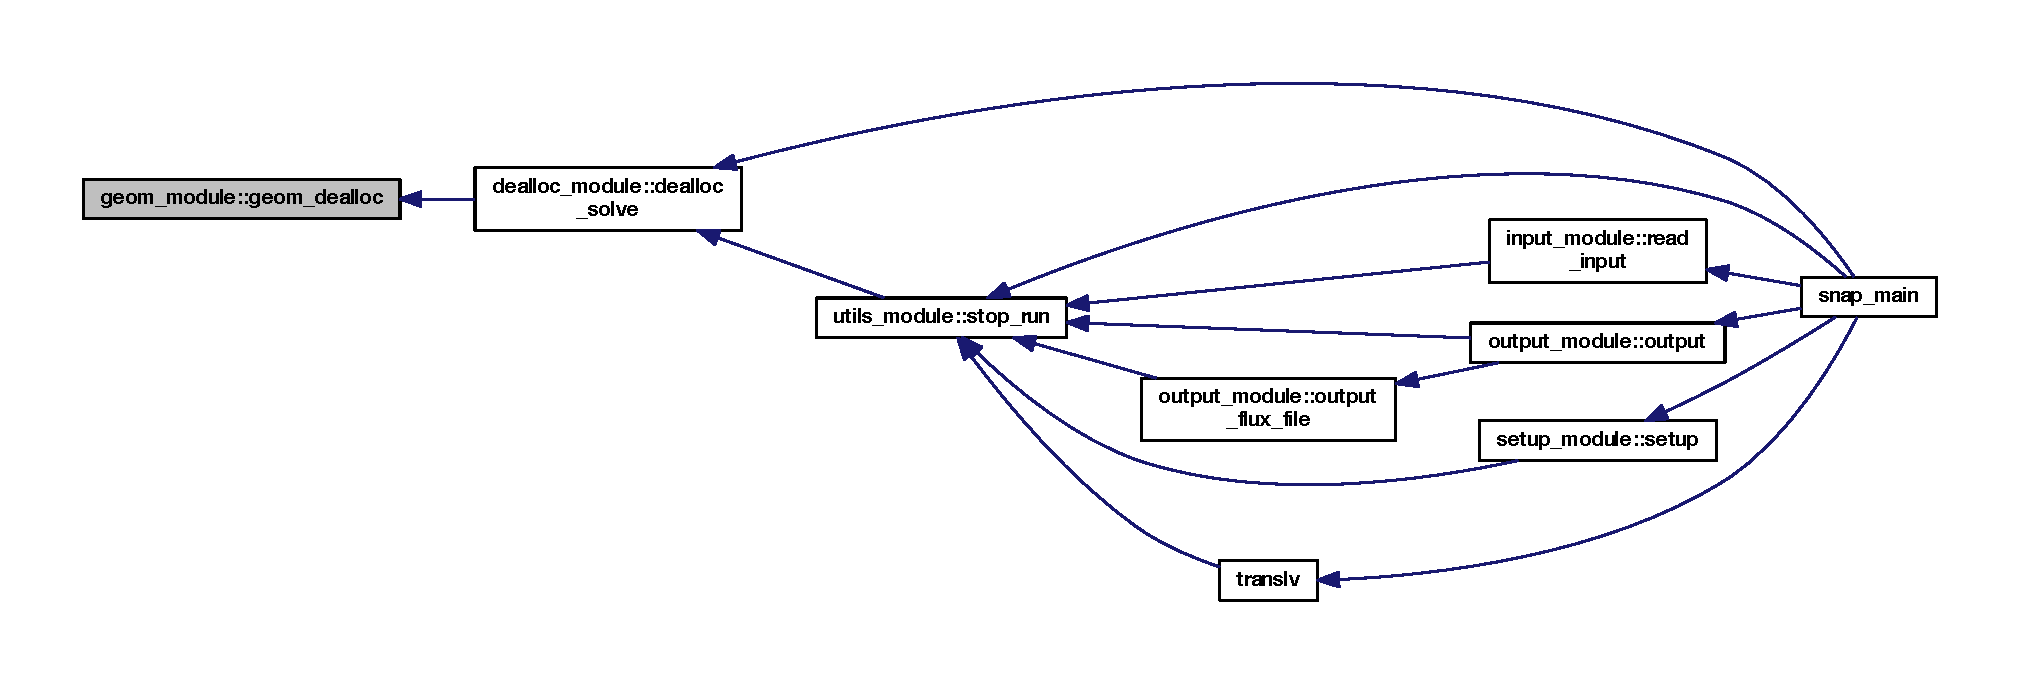
\includegraphics[width=350pt]{classgeom__module_ab2401a2eca471da4ca28fe634b5350d4_icgraph}
\end{center}
\end{figure}


\hypertarget{classgeom__module_aa09319572e809c686211758ef5fb129e}{\index{geom\-\_\-module@{geom\-\_\-module}!param\-\_\-calc@{param\-\_\-calc}}
\index{param\-\_\-calc@{param\-\_\-calc}!geom_module@{geom\-\_\-module}}
\subsubsection[{param\-\_\-calc}]{\setlength{\rightskip}{0pt plus 5cm}subroutine geom\-\_\-module\-::param\-\_\-calc (
\begin{DoxyParamCaption}
\item[{integer(i\-\_\-knd), intent(in)}]{ichunk, }
\item[{integer(i\-\_\-knd), intent(in)}]{nang, }
\item[{real(r\-\_\-knd), dimension(nang), intent(in)}]{mu, }
\item[{real(r\-\_\-knd), dimension(nang), intent(in)}]{eta, }
\item[{real(r\-\_\-knd), dimension(nang), intent(in)}]{xi, }
\item[{real(r\-\_\-knd), dimension({\bf nx},{\bf ny},{\bf nz}), intent(in)}]{cs, }
\item[{real(r\-\_\-knd), intent(in)}]{vd, }
\item[{real(r\-\_\-knd), dimension(nang,{\bf nx},{\bf ny},{\bf nz}), intent(out)}]{d}
\end{DoxyParamCaption}
)}}\label{classgeom__module_aa09319572e809c686211758ef5fb129e}


Definition at line 118 of file geom.\-f90.



Here is the caller graph for this function\-:\nopagebreak
\begin{figure}[H]
\begin{center}
\leavevmode
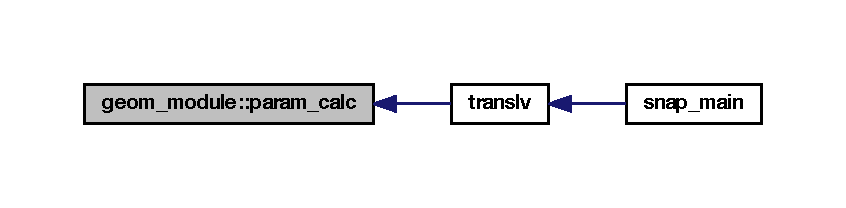
\includegraphics[width=350pt]{classgeom__module_aa09319572e809c686211758ef5fb129e_icgraph}
\end{center}
\end{figure}




\subsection{Member Data Documentation}
\hypertarget{classgeom__module_ae4c351982371a6870429ab660ec35e45}{\index{geom\-\_\-module@{geom\-\_\-module}!dinv@{dinv}}
\index{dinv@{dinv}!geom_module@{geom\-\_\-module}}
\subsubsection[{dinv}]{\setlength{\rightskip}{0pt plus 5cm}real(r\-\_\-knd), dimension(\-:,\-:,\-:,\-:,\-:), allocatable geom\-\_\-module\-::dinv}}\label{classgeom__module_ae4c351982371a6870429ab660ec35e45}


Definition at line 68 of file geom.\-f90.

\hypertarget{classgeom__module_a2f292c19b0e9bfc4cde1d54f0e9d4472}{\index{geom\-\_\-module@{geom\-\_\-module}!dx@{dx}}
\index{dx@{dx}!geom_module@{geom\-\_\-module}}
\subsubsection[{dx}]{\setlength{\rightskip}{0pt plus 5cm}real(r\-\_\-knd) geom\-\_\-module\-::dx}}\label{classgeom__module_a2f292c19b0e9bfc4cde1d54f0e9d4472}


Definition at line 64 of file geom.\-f90.

\hypertarget{classgeom__module_a13234163c83c1041d8053ab0f4ea5d40}{\index{geom\-\_\-module@{geom\-\_\-module}!dy@{dy}}
\index{dy@{dy}!geom_module@{geom\-\_\-module}}
\subsubsection[{dy}]{\setlength{\rightskip}{0pt plus 5cm}real(r\-\_\-knd) geom\-\_\-module\-::dy}}\label{classgeom__module_a13234163c83c1041d8053ab0f4ea5d40}


Definition at line 64 of file geom.\-f90.

\hypertarget{classgeom__module_a59842db695f66127f749bffd9df2f034}{\index{geom\-\_\-module@{geom\-\_\-module}!dz@{dz}}
\index{dz@{dz}!geom_module@{geom\-\_\-module}}
\subsubsection[{dz}]{\setlength{\rightskip}{0pt plus 5cm}real(r\-\_\-knd) geom\-\_\-module\-::dz}}\label{classgeom__module_a59842db695f66127f749bffd9df2f034}


Definition at line 64 of file geom.\-f90.

\hypertarget{classgeom__module_af657687714307a2bfe5e99ea8ee9f35e}{\index{geom\-\_\-module@{geom\-\_\-module}!hi@{hi}}
\index{hi@{hi}!geom_module@{geom\-\_\-module}}
\subsubsection[{hi}]{\setlength{\rightskip}{0pt plus 5cm}real(r\-\_\-knd) geom\-\_\-module\-::hi}}\label{classgeom__module_af657687714307a2bfe5e99ea8ee9f35e}


Definition at line 64 of file geom.\-f90.

\hypertarget{classgeom__module_ad5db4c62807a7025e92dd2c5742156eb}{\index{geom\-\_\-module@{geom\-\_\-module}!hj@{hj}}
\index{hj@{hj}!geom_module@{geom\-\_\-module}}
\subsubsection[{hj}]{\setlength{\rightskip}{0pt plus 5cm}real(r\-\_\-knd), dimension(\-:), allocatable geom\-\_\-module\-::hj}}\label{classgeom__module_ad5db4c62807a7025e92dd2c5742156eb}


Definition at line 66 of file geom.\-f90.

\hypertarget{classgeom__module_a42bd1a5bffae9b223ac63ce018664023}{\index{geom\-\_\-module@{geom\-\_\-module}!hk@{hk}}
\index{hk@{hk}!geom_module@{geom\-\_\-module}}
\subsubsection[{hk}]{\setlength{\rightskip}{0pt plus 5cm}real(r\-\_\-knd), dimension(\-:), allocatable geom\-\_\-module\-::hk}}\label{classgeom__module_a42bd1a5bffae9b223ac63ce018664023}


Definition at line 66 of file geom.\-f90.

\hypertarget{classgeom__module_a87c8f8859d2d98c1dfc36f0ccf4208df}{\index{geom\-\_\-module@{geom\-\_\-module}!jlb@{jlb}}
\index{jlb@{jlb}!geom_module@{geom\-\_\-module}}
\subsubsection[{jlb}]{\setlength{\rightskip}{0pt plus 5cm}integer(i\-\_\-knd) geom\-\_\-module\-::jlb}}\label{classgeom__module_a87c8f8859d2d98c1dfc36f0ccf4208df}


Definition at line 62 of file geom.\-f90.

\hypertarget{classgeom__module_ada7a9e753e21b30a06f0858f5deb4300}{\index{geom\-\_\-module@{geom\-\_\-module}!jub@{jub}}
\index{jub@{jub}!geom_module@{geom\-\_\-module}}
\subsubsection[{jub}]{\setlength{\rightskip}{0pt plus 5cm}integer(i\-\_\-knd) geom\-\_\-module\-::jub}}\label{classgeom__module_ada7a9e753e21b30a06f0858f5deb4300}


Definition at line 62 of file geom.\-f90.

\hypertarget{classgeom__module_a7c3abb8b57ed30570288a1da71db8444}{\index{geom\-\_\-module@{geom\-\_\-module}!klb@{klb}}
\index{klb@{klb}!geom_module@{geom\-\_\-module}}
\subsubsection[{klb}]{\setlength{\rightskip}{0pt plus 5cm}integer(i\-\_\-knd) geom\-\_\-module\-::klb}}\label{classgeom__module_a7c3abb8b57ed30570288a1da71db8444}


Definition at line 62 of file geom.\-f90.

\hypertarget{classgeom__module_a79842b1abc678e999d926bc361620371}{\index{geom\-\_\-module@{geom\-\_\-module}!kub@{kub}}
\index{kub@{kub}!geom_module@{geom\-\_\-module}}
\subsubsection[{kub}]{\setlength{\rightskip}{0pt plus 5cm}integer(i\-\_\-knd) geom\-\_\-module\-::kub}}\label{classgeom__module_a79842b1abc678e999d926bc361620371}


Definition at line 62 of file geom.\-f90.

\hypertarget{classgeom__module_a1fe9e4dc8297fc98198b561000a97973}{\index{geom\-\_\-module@{geom\-\_\-module}!lx@{lx}}
\index{lx@{lx}!geom_module@{geom\-\_\-module}}
\subsubsection[{lx}]{\setlength{\rightskip}{0pt plus 5cm}real(r\-\_\-knd) geom\-\_\-module\-::lx = one}}\label{classgeom__module_a1fe9e4dc8297fc98198b561000a97973}


Definition at line 37 of file geom.\-f90.

\hypertarget{classgeom__module_adc5d5005b562bb94578c33b5bcde0012}{\index{geom\-\_\-module@{geom\-\_\-module}!ly@{ly}}
\index{ly@{ly}!geom_module@{geom\-\_\-module}}
\subsubsection[{ly}]{\setlength{\rightskip}{0pt plus 5cm}real(r\-\_\-knd) geom\-\_\-module\-::ly = one}}\label{classgeom__module_adc5d5005b562bb94578c33b5bcde0012}


Definition at line 37 of file geom.\-f90.

\hypertarget{classgeom__module_aba080d6dd2b57ad40676a7331daaa824}{\index{geom\-\_\-module@{geom\-\_\-module}!lz@{lz}}
\index{lz@{lz}!geom_module@{geom\-\_\-module}}
\subsubsection[{lz}]{\setlength{\rightskip}{0pt plus 5cm}real(r\-\_\-knd) geom\-\_\-module\-::lz = one}}\label{classgeom__module_aba080d6dd2b57ad40676a7331daaa824}


Definition at line 37 of file geom.\-f90.

\hypertarget{classgeom__module_af92dc09eacd9c240bd51ea2792a13820}{\index{geom\-\_\-module@{geom\-\_\-module}!nc@{nc}}
\index{nc@{nc}!geom_module@{geom\-\_\-module}}
\subsubsection[{nc}]{\setlength{\rightskip}{0pt plus 5cm}integer(i\-\_\-knd) geom\-\_\-module\-::nc}}\label{classgeom__module_af92dc09eacd9c240bd51ea2792a13820}


Definition at line 62 of file geom.\-f90.

\hypertarget{classgeom__module_a764bf4ab4dc187512c803d73505e6b57}{\index{geom\-\_\-module@{geom\-\_\-module}!ndimen@{ndimen}}
\index{ndimen@{ndimen}!geom_module@{geom\-\_\-module}}
\subsubsection[{ndimen}]{\setlength{\rightskip}{0pt plus 5cm}integer(i\-\_\-knd) geom\-\_\-module\-::ndimen = 1}}\label{classgeom__module_a764bf4ab4dc187512c803d73505e6b57}


Definition at line 35 of file geom.\-f90.

\hypertarget{classgeom__module_a7a5902416f1d33e2a27620d6c82db061}{\index{geom\-\_\-module@{geom\-\_\-module}!nx@{nx}}
\index{nx@{nx}!geom_module@{geom\-\_\-module}}
\subsubsection[{nx}]{\setlength{\rightskip}{0pt plus 5cm}integer(i\-\_\-knd) geom\-\_\-module\-::nx = 4}}\label{classgeom__module_a7a5902416f1d33e2a27620d6c82db061}


Definition at line 35 of file geom.\-f90.

\hypertarget{classgeom__module_a38b87580d41ec11b8719f65f06b8b0a3}{\index{geom\-\_\-module@{geom\-\_\-module}!ny@{ny}}
\index{ny@{ny}!geom_module@{geom\-\_\-module}}
\subsubsection[{ny}]{\setlength{\rightskip}{0pt plus 5cm}integer(i\-\_\-knd) geom\-\_\-module\-::ny = 1}}\label{classgeom__module_a38b87580d41ec11b8719f65f06b8b0a3}


Definition at line 35 of file geom.\-f90.

\hypertarget{classgeom__module_a28abec0d4fe709bc64ee36b68347ce1a}{\index{geom\-\_\-module@{geom\-\_\-module}!ny\-\_\-gl@{ny\-\_\-gl}}
\index{ny\-\_\-gl@{ny\-\_\-gl}!geom_module@{geom\-\_\-module}}
\subsubsection[{ny\-\_\-gl}]{\setlength{\rightskip}{0pt plus 5cm}integer(i\-\_\-knd) geom\-\_\-module\-::ny\-\_\-gl}}\label{classgeom__module_a28abec0d4fe709bc64ee36b68347ce1a}


Definition at line 62 of file geom.\-f90.

\hypertarget{classgeom__module_a5f461a2f10c78de302a44c8c70b8fca5}{\index{geom\-\_\-module@{geom\-\_\-module}!nz@{nz}}
\index{nz@{nz}!geom_module@{geom\-\_\-module}}
\subsubsection[{nz}]{\setlength{\rightskip}{0pt plus 5cm}integer(i\-\_\-knd) geom\-\_\-module\-::nz = 1}}\label{classgeom__module_a5f461a2f10c78de302a44c8c70b8fca5}


Definition at line 35 of file geom.\-f90.

\hypertarget{classgeom__module_a3d237cf21a21064504566ce34b27c848}{\index{geom\-\_\-module@{geom\-\_\-module}!nz\-\_\-gl@{nz\-\_\-gl}}
\index{nz\-\_\-gl@{nz\-\_\-gl}!geom_module@{geom\-\_\-module}}
\subsubsection[{nz\-\_\-gl}]{\setlength{\rightskip}{0pt plus 5cm}integer(i\-\_\-knd) geom\-\_\-module\-::nz\-\_\-gl}}\label{classgeom__module_a3d237cf21a21064504566ce34b27c848}


Definition at line 62 of file geom.\-f90.



The documentation for this module was generated from the following file\-:\begin{DoxyCompactItemize}
\item 
src/\hyperlink{geom_8f90}{geom.\-f90}\end{DoxyCompactItemize}

\hypertarget{interfaceplib__module_1_1glmax}{\section{plib\-\_\-module\-:\-:glmax Interface Reference}
\label{interfaceplib__module_1_1glmax}\index{plib\-\_\-module\-::glmax@{plib\-\_\-module\-::glmax}}
}
\subsection*{Public Member Functions}
\begin{DoxyCompactItemize}
\item 
subroutine \hyperlink{interfaceplib__module_1_1glmax_a24ef7a1f27384c11193242febf4f0bd5}{glmax\-\_\-i} (value, comm)
\item 
subroutine \hyperlink{interfaceplib__module_1_1glmax_aa43d91838ba81256eeb45d848f9aa9cb}{glmax\-\_\-d} (value, comm)
\item 
subroutine \hyperlink{interfaceplib__module_1_1glmax_a3da7021412ef9237441dd3ca12dea228}{glmax\-\_\-d\-\_\-1d} (value, dlen, comm)
\end{DoxyCompactItemize}


\subsection{Detailed Description}


Definition at line 19 of file plib.\-f90.



\subsection{Member Function/\-Subroutine Documentation}
\hypertarget{interfaceplib__module_1_1glmax_aa43d91838ba81256eeb45d848f9aa9cb}{\index{plib\-\_\-module\-::glmax@{plib\-\_\-module\-::glmax}!glmax\-\_\-d@{glmax\-\_\-d}}
\index{glmax\-\_\-d@{glmax\-\_\-d}!plib_module::glmax@{plib\-\_\-module\-::glmax}}
\subsubsection[{glmax\-\_\-d}]{\setlength{\rightskip}{0pt plus 5cm}subroutine plib\-\_\-module\-::glmax\-::glmax\-\_\-d (
\begin{DoxyParamCaption}
\item[{real(r\-\_\-knd), intent(inout)}]{value, }
\item[{integer(i\-\_\-knd), intent(in)}]{comm}
\end{DoxyParamCaption}
)}}\label{interfaceplib__module_1_1glmax_aa43d91838ba81256eeb45d848f9aa9cb}


Definition at line 338 of file plib.\-f90.

\hypertarget{interfaceplib__module_1_1glmax_a3da7021412ef9237441dd3ca12dea228}{\index{plib\-\_\-module\-::glmax@{plib\-\_\-module\-::glmax}!glmax\-\_\-d\-\_\-1d@{glmax\-\_\-d\-\_\-1d}}
\index{glmax\-\_\-d\-\_\-1d@{glmax\-\_\-d\-\_\-1d}!plib_module::glmax@{plib\-\_\-module\-::glmax}}
\subsubsection[{glmax\-\_\-d\-\_\-1d}]{\setlength{\rightskip}{0pt plus 5cm}subroutine plib\-\_\-module\-::glmax\-::glmax\-\_\-d\-\_\-1d (
\begin{DoxyParamCaption}
\item[{real(r\-\_\-knd), dimension(dlen), intent(inout)}]{value, }
\item[{integer(i\-\_\-knd), intent(in)}]{dlen, }
\item[{integer(i\-\_\-knd), intent(in)}]{comm}
\end{DoxyParamCaption}
)}}\label{interfaceplib__module_1_1glmax_a3da7021412ef9237441dd3ca12dea228}


Definition at line 370 of file plib.\-f90.

\hypertarget{interfaceplib__module_1_1glmax_a24ef7a1f27384c11193242febf4f0bd5}{\index{plib\-\_\-module\-::glmax@{plib\-\_\-module\-::glmax}!glmax\-\_\-i@{glmax\-\_\-i}}
\index{glmax\-\_\-i@{glmax\-\_\-i}!plib_module::glmax@{plib\-\_\-module\-::glmax}}
\subsubsection[{glmax\-\_\-i}]{\setlength{\rightskip}{0pt plus 5cm}subroutine plib\-\_\-module\-::glmax\-::glmax\-\_\-i (
\begin{DoxyParamCaption}
\item[{integer(i\-\_\-knd), intent(inout)}]{value, }
\item[{integer(i\-\_\-knd), intent(in)}]{comm}
\end{DoxyParamCaption}
)}}\label{interfaceplib__module_1_1glmax_a24ef7a1f27384c11193242febf4f0bd5}


Definition at line 310 of file plib.\-f90.



The documentation for this interface was generated from the following file\-:\begin{DoxyCompactItemize}
\item 
src/\hyperlink{plib_8f90}{plib.\-f90}\end{DoxyCompactItemize}

\hypertarget{interfaceplib__module_1_1glmin}{\section{plib\-\_\-module\-:\-:glmin Interface Reference}
\label{interfaceplib__module_1_1glmin}\index{plib\-\_\-module\-::glmin@{plib\-\_\-module\-::glmin}}
}
\subsection*{Public Member Functions}
\begin{DoxyCompactItemize}
\item 
subroutine \hyperlink{interfaceplib__module_1_1glmin_ae1014cddf36aeba7a7f6920f52d38955}{glmin\-\_\-i} (value, comm)
\item 
subroutine \hyperlink{interfaceplib__module_1_1glmin_ab3d7b794de805d4a078126d9f302d9cd}{glmin\-\_\-d} (value, comm)
\end{DoxyCompactItemize}


\subsection{Detailed Description}


Definition at line 23 of file plib.\-f90.



\subsection{Member Function/\-Subroutine Documentation}
\hypertarget{interfaceplib__module_1_1glmin_ab3d7b794de805d4a078126d9f302d9cd}{\index{plib\-\_\-module\-::glmin@{plib\-\_\-module\-::glmin}!glmin\-\_\-d@{glmin\-\_\-d}}
\index{glmin\-\_\-d@{glmin\-\_\-d}!plib_module::glmin@{plib\-\_\-module\-::glmin}}
\subsubsection[{glmin\-\_\-d}]{\setlength{\rightskip}{0pt plus 5cm}subroutine plib\-\_\-module\-::glmin\-::glmin\-\_\-d (
\begin{DoxyParamCaption}
\item[{real(r\-\_\-knd), intent(inout)}]{value, }
\item[{integer(i\-\_\-knd), intent(in)}]{comm}
\end{DoxyParamCaption}
)}}\label{interfaceplib__module_1_1glmin_ab3d7b794de805d4a078126d9f302d9cd}


Definition at line 430 of file plib.\-f90.

\hypertarget{interfaceplib__module_1_1glmin_ae1014cddf36aeba7a7f6920f52d38955}{\index{plib\-\_\-module\-::glmin@{plib\-\_\-module\-::glmin}!glmin\-\_\-i@{glmin\-\_\-i}}
\index{glmin\-\_\-i@{glmin\-\_\-i}!plib_module::glmin@{plib\-\_\-module\-::glmin}}
\subsubsection[{glmin\-\_\-i}]{\setlength{\rightskip}{0pt plus 5cm}subroutine plib\-\_\-module\-::glmin\-::glmin\-\_\-i (
\begin{DoxyParamCaption}
\item[{integer(i\-\_\-knd), intent(inout)}]{value, }
\item[{integer(i\-\_\-knd), intent(in)}]{comm}
\end{DoxyParamCaption}
)}}\label{interfaceplib__module_1_1glmin_ae1014cddf36aeba7a7f6920f52d38955}


Definition at line 402 of file plib.\-f90.



The documentation for this interface was generated from the following file\-:\begin{DoxyCompactItemize}
\item 
src/\hyperlink{plib_8f90}{plib.\-f90}\end{DoxyCompactItemize}

\hypertarget{classglobal__module}{\section{global\-\_\-module Module Reference}
\label{classglobal__module}\index{global\-\_\-module@{global\-\_\-module}}
}
\subsection*{Public Attributes}
\begin{DoxyCompactItemize}
\item 
integer, parameter \hyperlink{classglobal__module_a968ba1aa6e3f1767b59bfb8bd310405e}{l\-\_\-knd} = K\-I\-N\-D( .T\-R\-U\-E. )
\item 
integer, parameter \hyperlink{classglobal__module_a01b861666154d8b3e5bd725ae8933438}{i\-\_\-knd} = S\-E\-L\-E\-C\-T\-E\-D\-\_\-\-I\-N\-T\-\_\-\-K\-I\-N\-D( 8 )
\item 
integer, parameter \hyperlink{classglobal__module_ab88bc58495adcaa0c39aac0c541fe8c8}{r\-\_\-knd} = S\-E\-L\-E\-C\-T\-E\-D\-\_\-\-R\-E\-A\-L\-\_\-\-K\-I\-N\-D( 13 )
\item 
character(len=16) \hyperlink{classglobal__module_a94b80c776276c5e9e870df62cdc27b1d}{ifile}
\item 
character(len=16) \hyperlink{classglobal__module_aa25a5f9ded0bd9460cc9a5c842a6812b}{ofile}
\item 
integer(\hyperlink{classglobal__module_a01b861666154d8b3e5bd725ae8933438}{i\-\_\-knd}), parameter \hyperlink{classglobal__module_a734e710669b353233ba6b431d2b10a60}{iunit} = 10
\item 
integer(\hyperlink{classglobal__module_a01b861666154d8b3e5bd725ae8933438}{i\-\_\-knd}), parameter \hyperlink{classglobal__module_a3d8941f8c329162cde48206e253955f5}{ounit} = 11
\item 
real(\hyperlink{classglobal__module_ab88bc58495adcaa0c39aac0c541fe8c8}{r\-\_\-knd}), parameter \hyperlink{classglobal__module_aee835b3a70993d265b7592f2485da98a}{zero} = 0.\-0\-\_\-r\-\_\-knd
\item 
real(\hyperlink{classglobal__module_ab88bc58495adcaa0c39aac0c541fe8c8}{r\-\_\-knd}), parameter \hyperlink{classglobal__module_aca3045154e42c1413c7e40cff43d609b}{half} = 0.\-5\-\_\-r\-\_\-knd
\item 
real(\hyperlink{classglobal__module_ab88bc58495adcaa0c39aac0c541fe8c8}{r\-\_\-knd}), parameter \hyperlink{classglobal__module_ad2273c99f1e5fd95558f9217ed48f65f}{one} = 1.\-0\-\_\-r\-\_\-knd
\item 
real(\hyperlink{classglobal__module_ab88bc58495adcaa0c39aac0c541fe8c8}{r\-\_\-knd}), parameter \hyperlink{classglobal__module_ae882a53fa5147b5a17b1de231a9edc1e}{two} = 2.\-0\-\_\-r\-\_\-knd
\item 
real(\hyperlink{classglobal__module_ab88bc58495adcaa0c39aac0c541fe8c8}{r\-\_\-knd}), parameter \hyperlink{classglobal__module_ac248f55c9fa522378b386ab9456aec4e}{pi} = 3.\-14159265358979\-\_\-r\-\_\-knd
\end{DoxyCompactItemize}


\subsection{Detailed Description}


Definition at line 1 of file global.\-f90.



\subsection{Member Data Documentation}
\hypertarget{classglobal__module_aca3045154e42c1413c7e40cff43d609b}{\index{global\-\_\-module@{global\-\_\-module}!half@{half}}
\index{half@{half}!global_module@{global\-\_\-module}}
\subsubsection[{half}]{\setlength{\rightskip}{0pt plus 5cm}real({\bf r\-\_\-knd}), parameter global\-\_\-module\-::half = 0.\-5\-\_\-r\-\_\-knd}}\label{classglobal__module_aca3045154e42c1413c7e40cff43d609b}


Definition at line 42 of file global.\-f90.

\hypertarget{classglobal__module_a01b861666154d8b3e5bd725ae8933438}{\index{global\-\_\-module@{global\-\_\-module}!i\-\_\-knd@{i\-\_\-knd}}
\index{i\-\_\-knd@{i\-\_\-knd}!global_module@{global\-\_\-module}}
\subsubsection[{i\-\_\-knd}]{\setlength{\rightskip}{0pt plus 5cm}integer, parameter global\-\_\-module\-::i\-\_\-knd = S\-E\-L\-E\-C\-T\-E\-D\-\_\-\-I\-N\-T\-\_\-\-K\-I\-N\-D( 8 )}}\label{classglobal__module_a01b861666154d8b3e5bd725ae8933438}


Definition at line 21 of file global.\-f90.

\hypertarget{classglobal__module_a94b80c776276c5e9e870df62cdc27b1d}{\index{global\-\_\-module@{global\-\_\-module}!ifile@{ifile}}
\index{ifile@{ifile}!global_module@{global\-\_\-module}}
\subsubsection[{ifile}]{\setlength{\rightskip}{0pt plus 5cm}character(len=16) global\-\_\-module\-::ifile}}\label{classglobal__module_a94b80c776276c5e9e870df62cdc27b1d}


Definition at line 33 of file global.\-f90.

\hypertarget{classglobal__module_a734e710669b353233ba6b431d2b10a60}{\index{global\-\_\-module@{global\-\_\-module}!iunit@{iunit}}
\index{iunit@{iunit}!global_module@{global\-\_\-module}}
\subsubsection[{iunit}]{\setlength{\rightskip}{0pt plus 5cm}integer({\bf i\-\_\-knd}), parameter global\-\_\-module\-::iunit = 10}}\label{classglobal__module_a734e710669b353233ba6b431d2b10a60}


Definition at line 35 of file global.\-f90.

\hypertarget{classglobal__module_a968ba1aa6e3f1767b59bfb8bd310405e}{\index{global\-\_\-module@{global\-\_\-module}!l\-\_\-knd@{l\-\_\-knd}}
\index{l\-\_\-knd@{l\-\_\-knd}!global_module@{global\-\_\-module}}
\subsubsection[{l\-\_\-knd}]{\setlength{\rightskip}{0pt plus 5cm}integer, parameter global\-\_\-module\-::l\-\_\-knd = K\-I\-N\-D( .T\-R\-U\-E. )}}\label{classglobal__module_a968ba1aa6e3f1767b59bfb8bd310405e}


Definition at line 20 of file global.\-f90.

\hypertarget{classglobal__module_aa25a5f9ded0bd9460cc9a5c842a6812b}{\index{global\-\_\-module@{global\-\_\-module}!ofile@{ofile}}
\index{ofile@{ofile}!global_module@{global\-\_\-module}}
\subsubsection[{ofile}]{\setlength{\rightskip}{0pt plus 5cm}character(len=16) global\-\_\-module\-::ofile}}\label{classglobal__module_aa25a5f9ded0bd9460cc9a5c842a6812b}


Definition at line 33 of file global.\-f90.

\hypertarget{classglobal__module_ad2273c99f1e5fd95558f9217ed48f65f}{\index{global\-\_\-module@{global\-\_\-module}!one@{one}}
\index{one@{one}!global_module@{global\-\_\-module}}
\subsubsection[{one}]{\setlength{\rightskip}{0pt plus 5cm}real({\bf r\-\_\-knd}), parameter global\-\_\-module\-::one = 1.\-0\-\_\-r\-\_\-knd}}\label{classglobal__module_ad2273c99f1e5fd95558f9217ed48f65f}


Definition at line 43 of file global.\-f90.

\hypertarget{classglobal__module_a3d8941f8c329162cde48206e253955f5}{\index{global\-\_\-module@{global\-\_\-module}!ounit@{ounit}}
\index{ounit@{ounit}!global_module@{global\-\_\-module}}
\subsubsection[{ounit}]{\setlength{\rightskip}{0pt plus 5cm}integer({\bf i\-\_\-knd}), parameter global\-\_\-module\-::ounit = 11}}\label{classglobal__module_a3d8941f8c329162cde48206e253955f5}


Definition at line 35 of file global.\-f90.

\hypertarget{classglobal__module_ac248f55c9fa522378b386ab9456aec4e}{\index{global\-\_\-module@{global\-\_\-module}!pi@{pi}}
\index{pi@{pi}!global_module@{global\-\_\-module}}
\subsubsection[{pi}]{\setlength{\rightskip}{0pt plus 5cm}real({\bf r\-\_\-knd}), parameter global\-\_\-module\-::pi = 3.\-14159265358979\-\_\-r\-\_\-knd}}\label{classglobal__module_ac248f55c9fa522378b386ab9456aec4e}


Definition at line 46 of file global.\-f90.

\hypertarget{classglobal__module_ab88bc58495adcaa0c39aac0c541fe8c8}{\index{global\-\_\-module@{global\-\_\-module}!r\-\_\-knd@{r\-\_\-knd}}
\index{r\-\_\-knd@{r\-\_\-knd}!global_module@{global\-\_\-module}}
\subsubsection[{r\-\_\-knd}]{\setlength{\rightskip}{0pt plus 5cm}integer, parameter global\-\_\-module\-::r\-\_\-knd = S\-E\-L\-E\-C\-T\-E\-D\-\_\-\-R\-E\-A\-L\-\_\-\-K\-I\-N\-D( 13 )}}\label{classglobal__module_ab88bc58495adcaa0c39aac0c541fe8c8}


Definition at line 22 of file global.\-f90.

\hypertarget{classglobal__module_ae882a53fa5147b5a17b1de231a9edc1e}{\index{global\-\_\-module@{global\-\_\-module}!two@{two}}
\index{two@{two}!global_module@{global\-\_\-module}}
\subsubsection[{two}]{\setlength{\rightskip}{0pt plus 5cm}real({\bf r\-\_\-knd}), parameter global\-\_\-module\-::two = 2.\-0\-\_\-r\-\_\-knd}}\label{classglobal__module_ae882a53fa5147b5a17b1de231a9edc1e}


Definition at line 44 of file global.\-f90.

\hypertarget{classglobal__module_aee835b3a70993d265b7592f2485da98a}{\index{global\-\_\-module@{global\-\_\-module}!zero@{zero}}
\index{zero@{zero}!global_module@{global\-\_\-module}}
\subsubsection[{zero}]{\setlength{\rightskip}{0pt plus 5cm}real({\bf r\-\_\-knd}), parameter global\-\_\-module\-::zero = 0.\-0\-\_\-r\-\_\-knd}}\label{classglobal__module_aee835b3a70993d265b7592f2485da98a}


Definition at line 41 of file global.\-f90.



The documentation for this module was generated from the following file\-:\begin{DoxyCompactItemize}
\item 
src/\hyperlink{global_8f90}{global.\-f90}\end{DoxyCompactItemize}

\hypertarget{classinner__module}{\section{inner\-\_\-module Module Reference}
\label{classinner__module}\index{inner\-\_\-module@{inner\-\_\-module}}
}
\subsection*{Public Member Functions}
\begin{DoxyCompactItemize}
\item 
subroutine, public \hyperlink{classinner__module_a350653dec40b4e680597662f0f71152a}{inner} (inno, iits)
\end{DoxyCompactItemize}
\subsection*{Private Member Functions}
\begin{DoxyCompactItemize}
\item 
subroutine \hyperlink{classinner__module_a54814aa404076eeef0878195e857c6dc}{inr\-\_\-src}
\item 
subroutine \hyperlink{classinner__module_ab4e7dc903de165ff491549c87e4d886b}{inr\-\_\-src\-\_\-scat} (qo, cs, f, fm, q)
\item 
subroutine \hyperlink{classinner__module_aedc12f5460b9dd44814f2bd38158cc60}{inr\-\_\-conv} (inno, iits)
\end{DoxyCompactItemize}


\subsection{Detailed Description}


Definition at line 1 of file inner.\-f90.



\subsection{Member Function/\-Subroutine Documentation}
\hypertarget{classinner__module_a350653dec40b4e680597662f0f71152a}{\index{inner\-\_\-module@{inner\-\_\-module}!inner@{inner}}
\index{inner@{inner}!inner_module@{inner\-\_\-module}}
\subsubsection[{inner}]{\setlength{\rightskip}{0pt plus 5cm}subroutine, public inner\-\_\-module\-::inner (
\begin{DoxyParamCaption}
\item[{integer(i\-\_\-knd), intent(in)}]{inno, }
\item[{integer(i\-\_\-knd), dimension(ng), intent(out)}]{iits}
\end{DoxyParamCaption}
)}}\label{classinner__module_a350653dec40b4e680597662f0f71152a}


Definition at line 40 of file inner.\-f90.



Here is the call graph for this function\-:\nopagebreak
\begin{figure}[H]
\begin{center}
\leavevmode
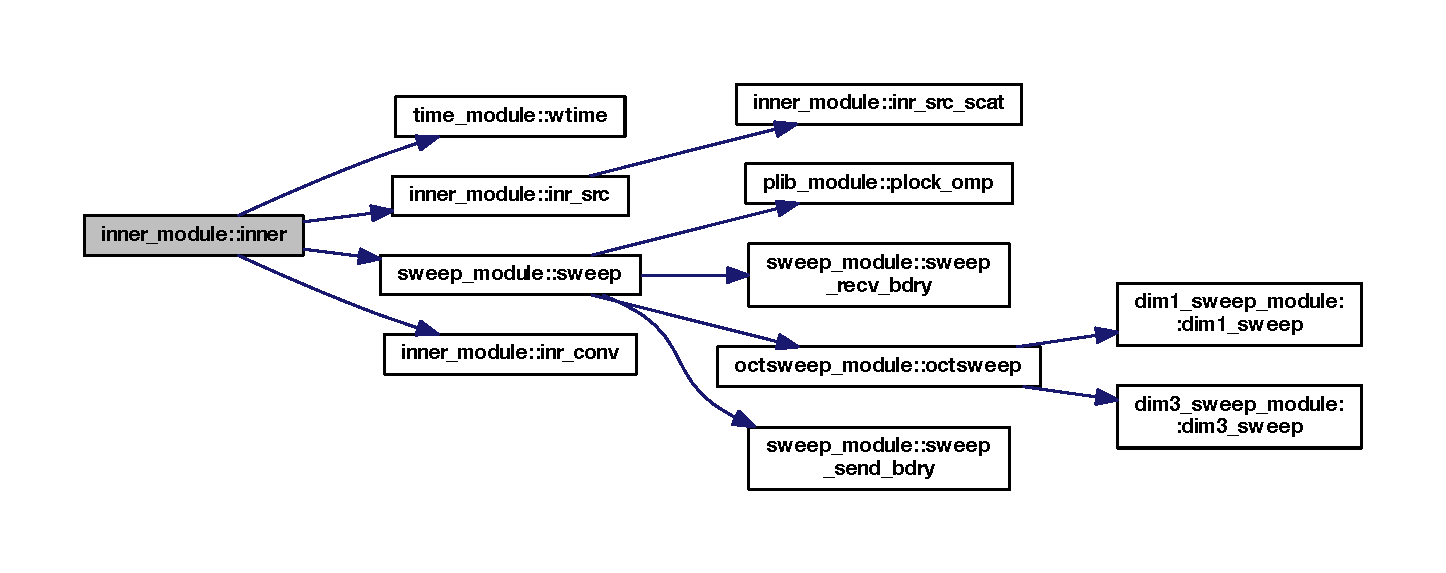
\includegraphics[width=350pt]{classinner__module_a350653dec40b4e680597662f0f71152a_cgraph}
\end{center}
\end{figure}




Here is the caller graph for this function\-:\nopagebreak
\begin{figure}[H]
\begin{center}
\leavevmode
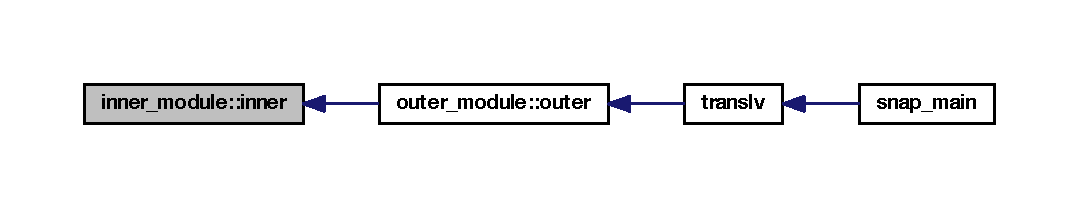
\includegraphics[width=350pt]{classinner__module_a350653dec40b4e680597662f0f71152a_icgraph}
\end{center}
\end{figure}


\hypertarget{classinner__module_aedc12f5460b9dd44814f2bd38158cc60}{\index{inner\-\_\-module@{inner\-\_\-module}!inr\-\_\-conv@{inr\-\_\-conv}}
\index{inr\-\_\-conv@{inr\-\_\-conv}!inner_module@{inner\-\_\-module}}
\subsubsection[{inr\-\_\-conv}]{\setlength{\rightskip}{0pt plus 5cm}subroutine inner\-\_\-module\-::inr\-\_\-conv (
\begin{DoxyParamCaption}
\item[{integer(i\-\_\-knd), intent(in)}]{inno, }
\item[{integer(i\-\_\-knd), dimension(ng), intent(out)}]{iits}
\end{DoxyParamCaption}
)\hspace{0.3cm}{\ttfamily [private]}}}\label{classinner__module_aedc12f5460b9dd44814f2bd38158cc60}


Definition at line 192 of file inner.\-f90.



Here is the caller graph for this function\-:\nopagebreak
\begin{figure}[H]
\begin{center}
\leavevmode
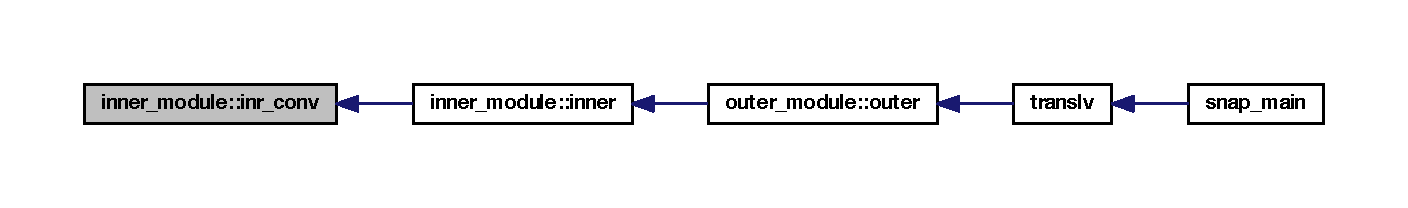
\includegraphics[width=350pt]{classinner__module_aedc12f5460b9dd44814f2bd38158cc60_icgraph}
\end{center}
\end{figure}


\hypertarget{classinner__module_a54814aa404076eeef0878195e857c6dc}{\index{inner\-\_\-module@{inner\-\_\-module}!inr\-\_\-src@{inr\-\_\-src}}
\index{inr\-\_\-src@{inr\-\_\-src}!inner_module@{inner\-\_\-module}}
\subsubsection[{inr\-\_\-src}]{\setlength{\rightskip}{0pt plus 5cm}subroutine inner\-\_\-module\-::inr\-\_\-src (
\begin{DoxyParamCaption}
{}
\end{DoxyParamCaption}
)\hspace{0.3cm}{\ttfamily [private]}}}\label{classinner__module_a54814aa404076eeef0878195e857c6dc}


Definition at line 103 of file inner.\-f90.



Here is the call graph for this function\-:\nopagebreak
\begin{figure}[H]
\begin{center}
\leavevmode
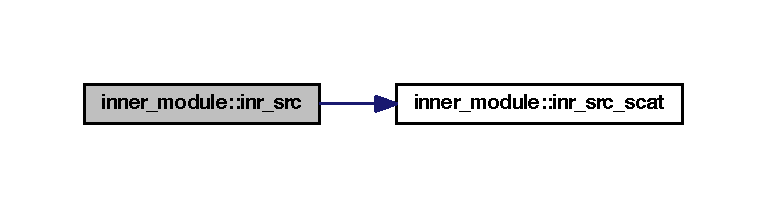
\includegraphics[width=350pt]{classinner__module_a54814aa404076eeef0878195e857c6dc_cgraph}
\end{center}
\end{figure}




Here is the caller graph for this function\-:\nopagebreak
\begin{figure}[H]
\begin{center}
\leavevmode
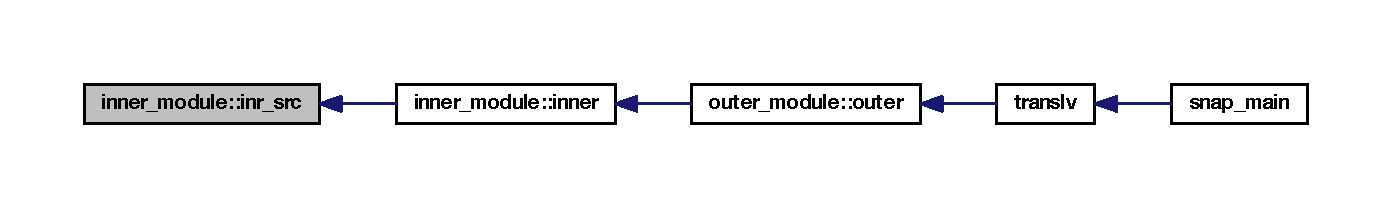
\includegraphics[width=350pt]{classinner__module_a54814aa404076eeef0878195e857c6dc_icgraph}
\end{center}
\end{figure}


\hypertarget{classinner__module_ab4e7dc903de165ff491549c87e4d886b}{\index{inner\-\_\-module@{inner\-\_\-module}!inr\-\_\-src\-\_\-scat@{inr\-\_\-src\-\_\-scat}}
\index{inr\-\_\-src\-\_\-scat@{inr\-\_\-src\-\_\-scat}!inner_module@{inner\-\_\-module}}
\subsubsection[{inr\-\_\-src\-\_\-scat}]{\setlength{\rightskip}{0pt plus 5cm}subroutine inner\-\_\-module\-::inr\-\_\-src\-\_\-scat (
\begin{DoxyParamCaption}
\item[{real(r\-\_\-knd), dimension(cmom,nx,ny,nz), intent(in)}]{qo, }
\item[{real(r\-\_\-knd), dimension(nmom,nx,ny,nz), intent(in)}]{cs, }
\item[{real(r\-\_\-knd), dimension(nx,ny,nz), intent(in)}]{f, }
\item[{real(r\-\_\-knd), dimension(cmom-\/1,nx,ny,nz), intent(in)}]{fm, }
\item[{real(r\-\_\-knd), dimension(cmom,nx,ny,nz), intent(out)}]{q}
\end{DoxyParamCaption}
)\hspace{0.3cm}{\ttfamily [private]}}}\label{classinner__module_ab4e7dc903de165ff491549c87e4d886b}


Definition at line 134 of file inner.\-f90.



Here is the caller graph for this function\-:\nopagebreak
\begin{figure}[H]
\begin{center}
\leavevmode
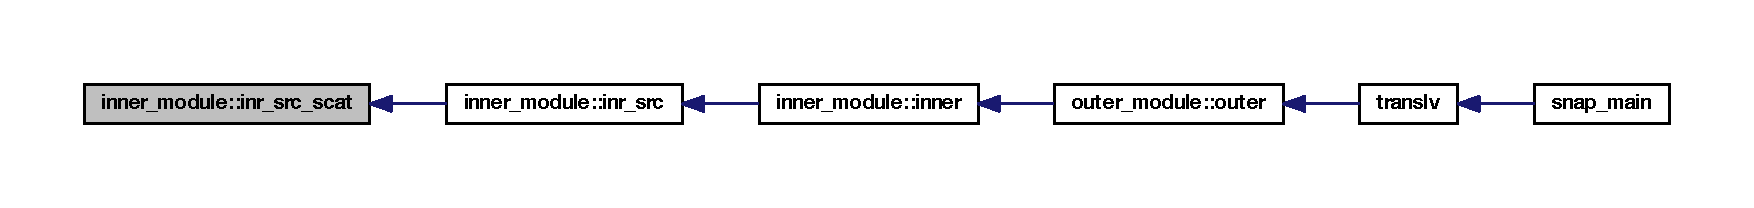
\includegraphics[width=350pt]{classinner__module_ab4e7dc903de165ff491549c87e4d886b_icgraph}
\end{center}
\end{figure}




The documentation for this module was generated from the following file\-:\begin{DoxyCompactItemize}
\item 
src/\hyperlink{inner_8f90}{inner.\-f90}\end{DoxyCompactItemize}

\hypertarget{classinput__module}{\section{input\-\_\-module Module Reference}
\label{classinput__module}\index{input\-\_\-module@{input\-\_\-module}}
}


This module controls the reading of the input file and checking the input parameters for acceptable values.  


\subsection*{Public Member Functions}
\begin{DoxyCompactItemize}
\item 
subroutine, public \hyperlink{classinput__module_a2be72b2b78d8f4e7fc02f147743c398c}{read\-\_\-input}
\end{DoxyCompactItemize}
\subsection*{Private Member Functions}
\begin{DoxyCompactItemize}
\item 
subroutine \hyperlink{classinput__module_ade4ea3790165f2f6d2d89ac453bdc0c0}{input\-\_\-echo}
\item 
subroutine \hyperlink{classinput__module_a0877bfa4c3658948884bcad75a3d133d}{input\-\_\-check} (ierr)
\item 
subroutine \hyperlink{classinput__module_ab4dc0d3c037cf364f55637634e4a9c0b}{var\-\_\-bcast}
\end{DoxyCompactItemize}


\subsection{Detailed Description}
This module controls the reading of the input file and checking the input parameters for acceptable values. 

Definition at line 10 of file input.\-f90.



\subsection{Member Function/\-Subroutine Documentation}
\hypertarget{classinput__module_a0877bfa4c3658948884bcad75a3d133d}{\index{input\-\_\-module@{input\-\_\-module}!input\-\_\-check@{input\-\_\-check}}
\index{input\-\_\-check@{input\-\_\-check}!input_module@{input\-\_\-module}}
\subsubsection[{input\-\_\-check}]{\setlength{\rightskip}{0pt plus 5cm}subroutine input\-\_\-module\-::input\-\_\-check (
\begin{DoxyParamCaption}
\item[{integer(i\-\_\-knd), intent(inout)}]{ierr}
\end{DoxyParamCaption}
)\hspace{0.3cm}{\ttfamily [private]}}}\label{classinput__module_a0877bfa4c3658948884bcad75a3d133d}


Definition at line 180 of file input.\-f90.



Here is the call graph for this function\-:\nopagebreak
\begin{figure}[H]
\begin{center}
\leavevmode
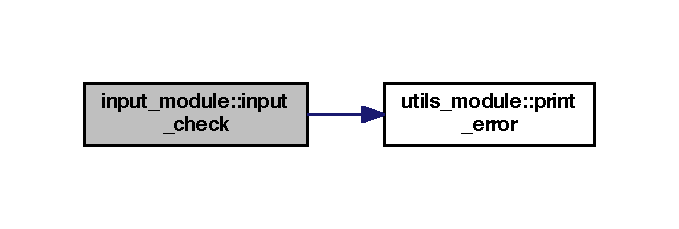
\includegraphics[width=326pt]{classinput__module_a0877bfa4c3658948884bcad75a3d133d_cgraph}
\end{center}
\end{figure}




Here is the caller graph for this function\-:\nopagebreak
\begin{figure}[H]
\begin{center}
\leavevmode
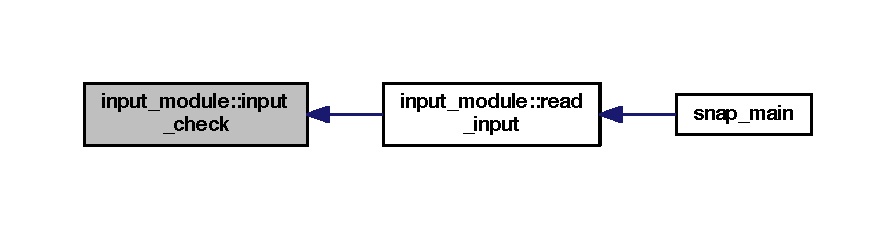
\includegraphics[width=350pt]{classinput__module_a0877bfa4c3658948884bcad75a3d133d_icgraph}
\end{center}
\end{figure}


\hypertarget{classinput__module_ade4ea3790165f2f6d2d89ac453bdc0c0}{\index{input\-\_\-module@{input\-\_\-module}!input\-\_\-echo@{input\-\_\-echo}}
\index{input\-\_\-echo@{input\-\_\-echo}!input_module@{input\-\_\-module}}
\subsubsection[{input\-\_\-echo}]{\setlength{\rightskip}{0pt plus 5cm}subroutine input\-\_\-module\-::input\-\_\-echo (
\begin{DoxyParamCaption}
{}
\end{DoxyParamCaption}
)\hspace{0.3cm}{\ttfamily [private]}}}\label{classinput__module_ade4ea3790165f2f6d2d89ac453bdc0c0}


Definition at line 106 of file input.\-f90.



Here is the caller graph for this function\-:\nopagebreak
\begin{figure}[H]
\begin{center}
\leavevmode
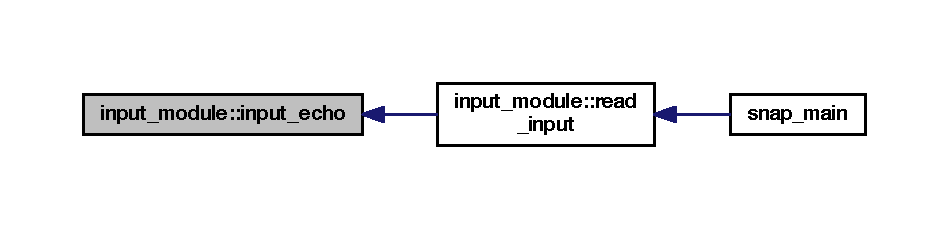
\includegraphics[width=350pt]{classinput__module_ade4ea3790165f2f6d2d89ac453bdc0c0_icgraph}
\end{center}
\end{figure}


\hypertarget{classinput__module_a2be72b2b78d8f4e7fc02f147743c398c}{\index{input\-\_\-module@{input\-\_\-module}!read\-\_\-input@{read\-\_\-input}}
\index{read\-\_\-input@{read\-\_\-input}!input_module@{input\-\_\-module}}
\subsubsection[{read\-\_\-input}]{\setlength{\rightskip}{0pt plus 5cm}subroutine, public input\-\_\-module\-::read\-\_\-input (
\begin{DoxyParamCaption}
{}
\end{DoxyParamCaption}
)}}\label{classinput__module_a2be72b2b78d8f4e7fc02f147743c398c}


Definition at line 40 of file input.\-f90.



Here is the call graph for this function\-:\nopagebreak
\begin{figure}[H]
\begin{center}
\leavevmode
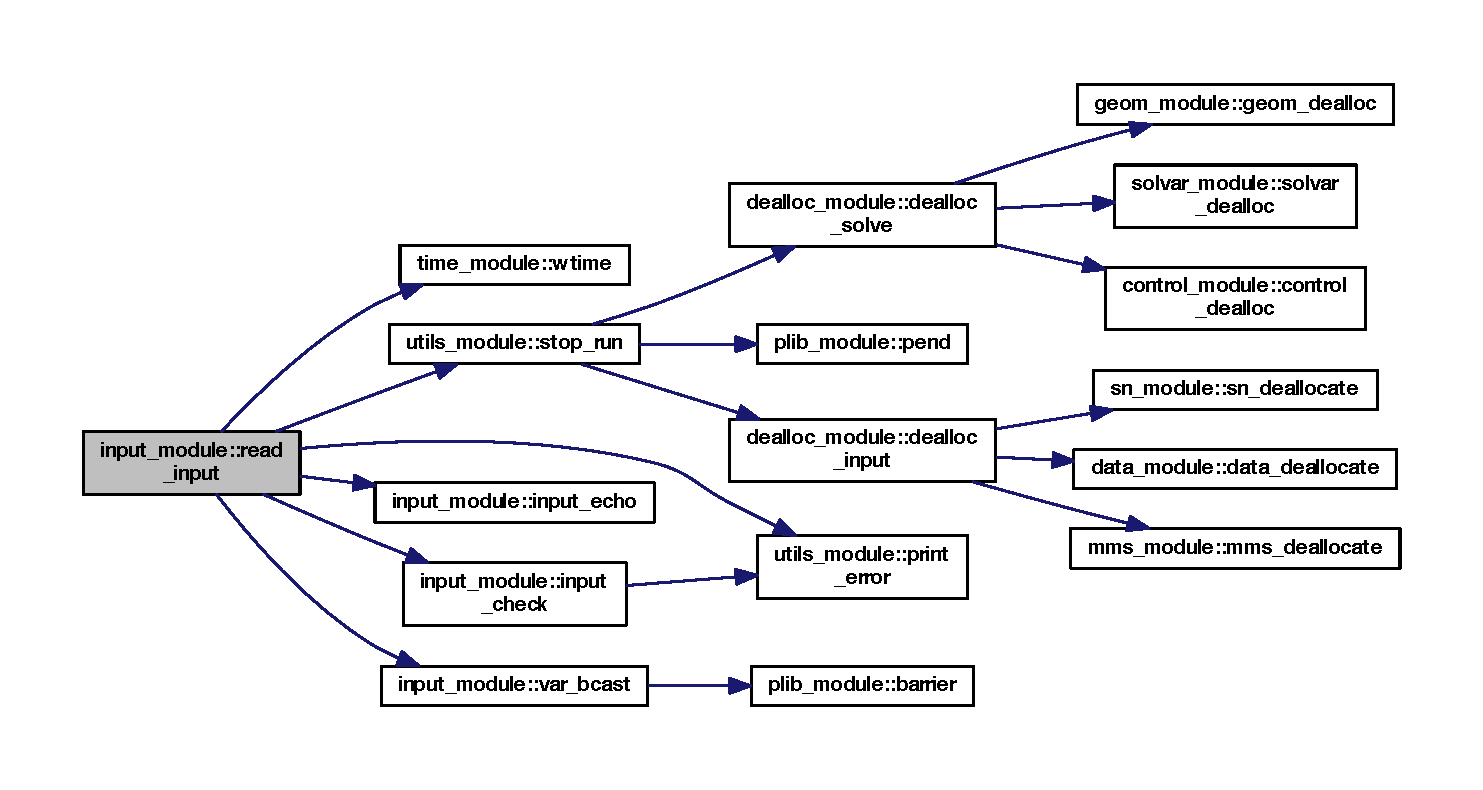
\includegraphics[width=350pt]{classinput__module_a2be72b2b78d8f4e7fc02f147743c398c_cgraph}
\end{center}
\end{figure}




Here is the caller graph for this function\-:\nopagebreak
\begin{figure}[H]
\begin{center}
\leavevmode
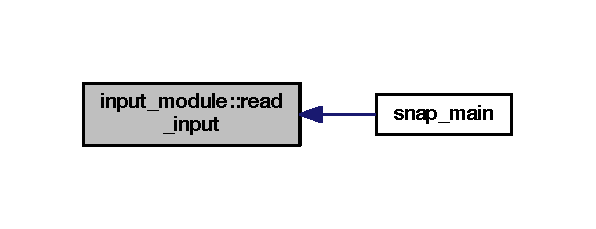
\includegraphics[width=286pt]{classinput__module_a2be72b2b78d8f4e7fc02f147743c398c_icgraph}
\end{center}
\end{figure}


\hypertarget{classinput__module_ab4dc0d3c037cf364f55637634e4a9c0b}{\index{input\-\_\-module@{input\-\_\-module}!var\-\_\-bcast@{var\-\_\-bcast}}
\index{var\-\_\-bcast@{var\-\_\-bcast}!input_module@{input\-\_\-module}}
\subsubsection[{var\-\_\-bcast}]{\setlength{\rightskip}{0pt plus 5cm}subroutine input\-\_\-module\-::var\-\_\-bcast (
\begin{DoxyParamCaption}
{}
\end{DoxyParamCaption}
)\hspace{0.3cm}{\ttfamily [private]}}}\label{classinput__module_ab4dc0d3c037cf364f55637634e4a9c0b}


Definition at line 476 of file input.\-f90.



Here is the call graph for this function\-:\nopagebreak
\begin{figure}[H]
\begin{center}
\leavevmode
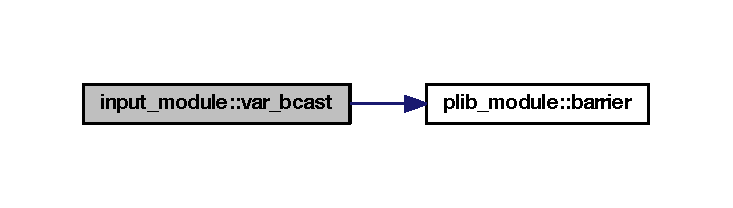
\includegraphics[width=350pt]{classinput__module_ab4dc0d3c037cf364f55637634e4a9c0b_cgraph}
\end{center}
\end{figure}




Here is the caller graph for this function\-:\nopagebreak
\begin{figure}[H]
\begin{center}
\leavevmode
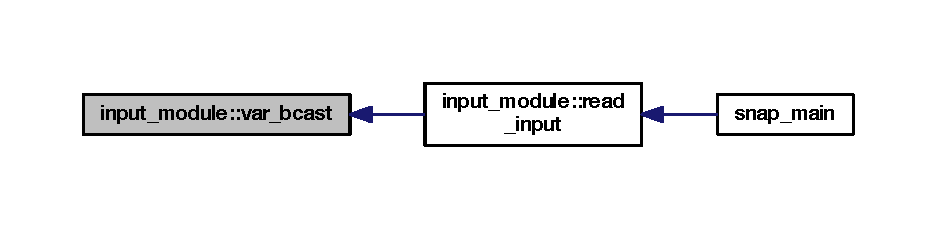
\includegraphics[width=350pt]{classinput__module_ab4dc0d3c037cf364f55637634e4a9c0b_icgraph}
\end{center}
\end{figure}




The documentation for this module was generated from the following file\-:\begin{DoxyCompactItemize}
\item 
src/\hyperlink{input_8f90}{input.\-f90}\end{DoxyCompactItemize}

\hypertarget{classmms__module}{\section{mms\-\_\-module Module Reference}
\label{classmms__module}\index{mms\-\_\-module@{mms\-\_\-module}}
}


This module contains all the setup and verification subroutines for code verification with M\-M\-S.  


\subsection*{Public Member Functions}
\begin{DoxyCompactItemize}
\item 
subroutine, public \hyperlink{classmms__module_af6e2504f62297dcb69f3939549152fef}{mms\-\_\-setup} (ierr, error)
\item 
subroutine, public \hyperlink{classmms__module_ae6195b5333d8369babda3da8875a6f22}{mms\-\_\-deallocate}
\item 
subroutine, public \hyperlink{classmms__module_a37e1faf94ca3526af48c3e8efc1d332a}{mms\-\_\-verify\-\_\-1} (flux)
\end{DoxyCompactItemize}
\subsection*{Public Attributes}
\begin{DoxyCompactItemize}
\item 
real(r\-\_\-knd), dimension(\-:,\-:,\-:,\-:), \\*
allocatable, public \hyperlink{classmms__module_a20157f9a49b1c0b449c340b7b1a63791}{ref\-\_\-flux}
\item 
real(r\-\_\-knd), dimension(\-:,\-:,\-:,\-:,\-:), \\*
allocatable, public \hyperlink{classmms__module_aaa592b5b9f1591e2a34df390563b0c56}{ref\-\_\-fluxm}
\end{DoxyCompactItemize}
\subsection*{Private Member Functions}
\begin{DoxyCompactItemize}
\item 
subroutine \hyperlink{classmms__module_ab75ca017795268e2e798920ed82058c0}{mms\-\_\-allocate} (ierr, error)
\item 
subroutine \hyperlink{classmms__module_a62f471d104fd6b83a9a0649115e4103e}{mms\-\_\-cells}
\item 
subroutine \hyperlink{classmms__module_a7182d71cc52a5cb7402d649bb17b0af9}{mms\-\_\-flux\-\_\-1}
\item 
subroutine \hyperlink{classmms__module_a92298f4f6f9a03d54169aee15197f591}{mms\-\_\-trigint} (trig, lc, d, del, cb, fn)
\item 
subroutine \hyperlink{classmms__module_aa571bba8b81b30ec0d1560f2d6bd4e2a}{mms\-\_\-src\-\_\-1}
\item 
subroutine \hyperlink{classmms__module_a8ed588a3dafe93834940e9df3460969b}{mms\-\_\-flux\-\_\-1\-\_\-2}
\end{DoxyCompactItemize}
\subsection*{Private Attributes}
\begin{DoxyCompactItemize}
\item 
real(r\-\_\-knd) \hyperlink{classmms__module_a874f8531253686519c7dd40848edbc00}{a}
\item 
real(r\-\_\-knd) \hyperlink{classmms__module_adb85ae57ca25aea5f2e91f7df6d53dc1}{b}
\item 
real(r\-\_\-knd) \hyperlink{classmms__module_a6bd089f9df8ee45c901b6830eca017f6}{c}
\item 
real(r\-\_\-knd), dimension(\-:), \\*
allocatable \hyperlink{classmms__module_aaca218de11850fada15be6a3bbeb5159}{ib}
\item 
real(r\-\_\-knd), dimension(\-:), \\*
allocatable \hyperlink{classmms__module_a53a60661b3d933e48dbf0a926a4b010c}{jb}
\item 
real(r\-\_\-knd), dimension(\-:), \\*
allocatable \hyperlink{classmms__module_a634bb1d1d1405007f6bec01e8b6d9b85}{kb}
\end{DoxyCompactItemize}


\subsection{Detailed Description}
This module contains all the setup and verification subroutines for code verification with M\-M\-S. 

Definition at line 10 of file mms.\-f90.



\subsection{Member Function/\-Subroutine Documentation}
\hypertarget{classmms__module_ab75ca017795268e2e798920ed82058c0}{\index{mms\-\_\-module@{mms\-\_\-module}!mms\-\_\-allocate@{mms\-\_\-allocate}}
\index{mms\-\_\-allocate@{mms\-\_\-allocate}!mms_module@{mms\-\_\-module}}
\subsubsection[{mms\-\_\-allocate}]{\setlength{\rightskip}{0pt plus 5cm}subroutine mms\-\_\-module\-::mms\-\_\-allocate (
\begin{DoxyParamCaption}
\item[{integer(i\-\_\-knd), intent(out)}]{ierr, }
\item[{character(len=64), intent(out)}]{error}
\end{DoxyParamCaption}
)\hspace{0.3cm}{\ttfamily [private]}}}\label{classmms__module_ab75ca017795268e2e798920ed82058c0}


Definition at line 120 of file mms.\-f90.



Here is the caller graph for this function\-:\nopagebreak
\begin{figure}[H]
\begin{center}
\leavevmode
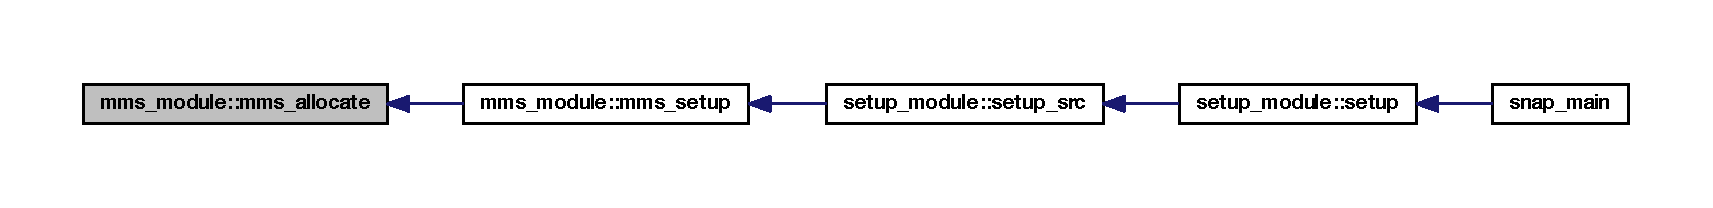
\includegraphics[width=350pt]{classmms__module_ab75ca017795268e2e798920ed82058c0_icgraph}
\end{center}
\end{figure}


\hypertarget{classmms__module_a62f471d104fd6b83a9a0649115e4103e}{\index{mms\-\_\-module@{mms\-\_\-module}!mms\-\_\-cells@{mms\-\_\-cells}}
\index{mms\-\_\-cells@{mms\-\_\-cells}!mms_module@{mms\-\_\-module}}
\subsubsection[{mms\-\_\-cells}]{\setlength{\rightskip}{0pt plus 5cm}subroutine mms\-\_\-module\-::mms\-\_\-cells (
\begin{DoxyParamCaption}
{}
\end{DoxyParamCaption}
)\hspace{0.3cm}{\ttfamily [private]}}}\label{classmms__module_a62f471d104fd6b83a9a0649115e4103e}


Definition at line 175 of file mms.\-f90.



Here is the caller graph for this function\-:\nopagebreak
\begin{figure}[H]
\begin{center}
\leavevmode
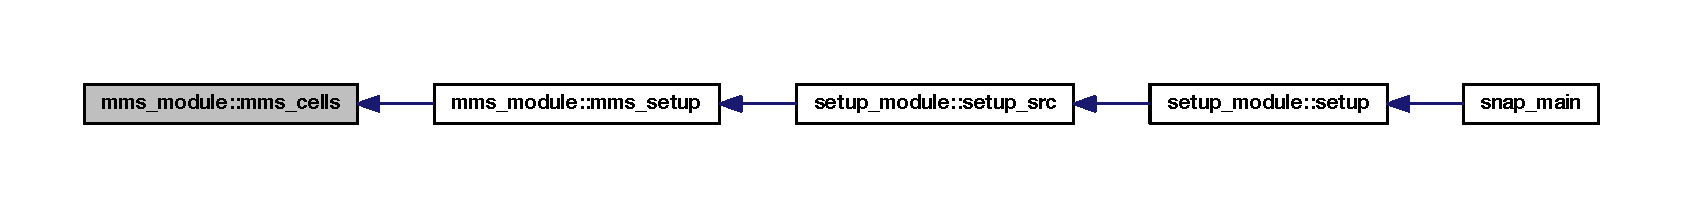
\includegraphics[width=350pt]{classmms__module_a62f471d104fd6b83a9a0649115e4103e_icgraph}
\end{center}
\end{figure}


\hypertarget{classmms__module_ae6195b5333d8369babda3da8875a6f22}{\index{mms\-\_\-module@{mms\-\_\-module}!mms\-\_\-deallocate@{mms\-\_\-deallocate}}
\index{mms\-\_\-deallocate@{mms\-\_\-deallocate}!mms_module@{mms\-\_\-module}}
\subsubsection[{mms\-\_\-deallocate}]{\setlength{\rightskip}{0pt plus 5cm}subroutine, public mms\-\_\-module\-::mms\-\_\-deallocate (
\begin{DoxyParamCaption}
{}
\end{DoxyParamCaption}
)}}\label{classmms__module_ae6195b5333d8369babda3da8875a6f22}


Definition at line 155 of file mms.\-f90.



Here is the caller graph for this function\-:\nopagebreak
\begin{figure}[H]
\begin{center}
\leavevmode
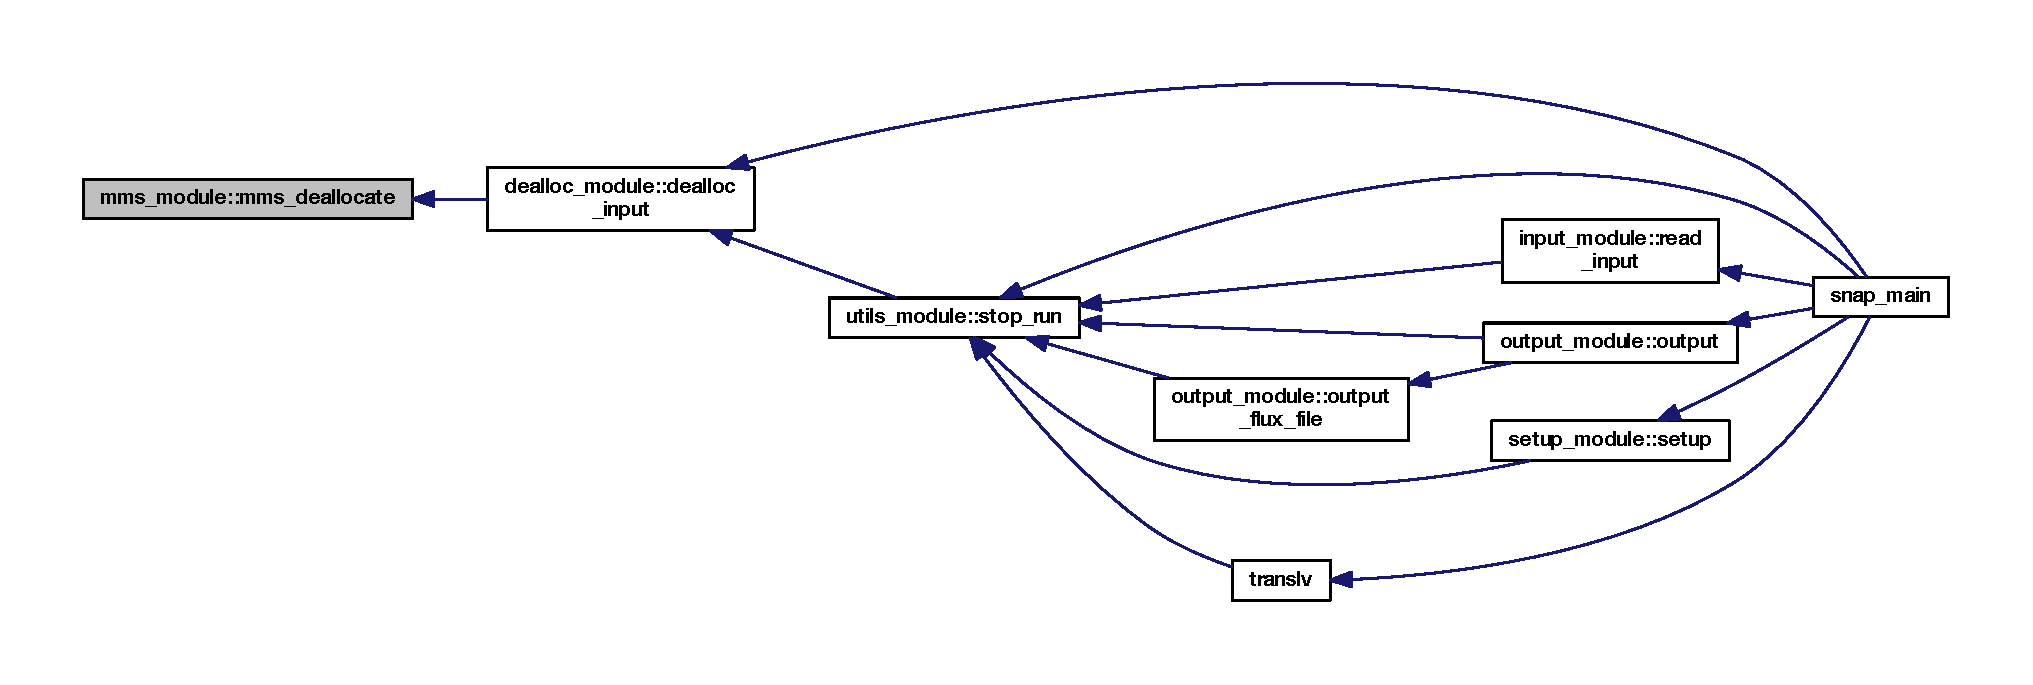
\includegraphics[width=350pt]{classmms__module_ae6195b5333d8369babda3da8875a6f22_icgraph}
\end{center}
\end{figure}


\hypertarget{classmms__module_a7182d71cc52a5cb7402d649bb17b0af9}{\index{mms\-\_\-module@{mms\-\_\-module}!mms\-\_\-flux\-\_\-1@{mms\-\_\-flux\-\_\-1}}
\index{mms\-\_\-flux\-\_\-1@{mms\-\_\-flux\-\_\-1}!mms_module@{mms\-\_\-module}}
\subsubsection[{mms\-\_\-flux\-\_\-1}]{\setlength{\rightskip}{0pt plus 5cm}subroutine mms\-\_\-module\-::mms\-\_\-flux\-\_\-1 (
\begin{DoxyParamCaption}
{}
\end{DoxyParamCaption}
)\hspace{0.3cm}{\ttfamily [private]}}}\label{classmms__module_a7182d71cc52a5cb7402d649bb17b0af9}


Definition at line 219 of file mms.\-f90.



Here is the call graph for this function\-:\nopagebreak
\begin{figure}[H]
\begin{center}
\leavevmode
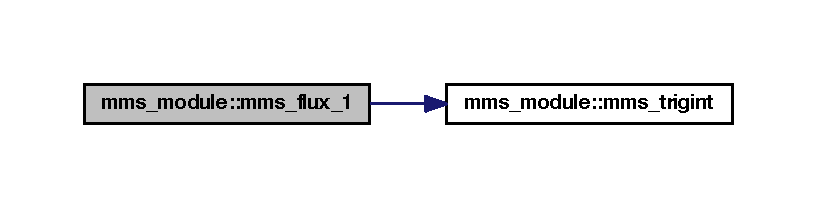
\includegraphics[width=350pt]{classmms__module_a7182d71cc52a5cb7402d649bb17b0af9_cgraph}
\end{center}
\end{figure}




Here is the caller graph for this function\-:\nopagebreak
\begin{figure}[H]
\begin{center}
\leavevmode
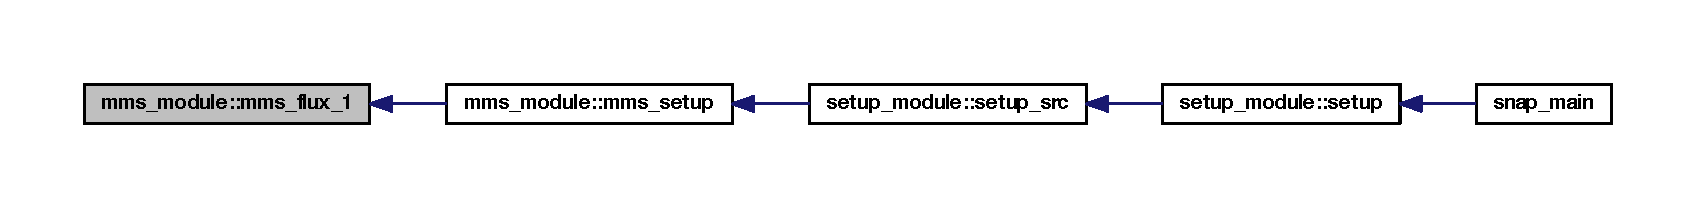
\includegraphics[width=350pt]{classmms__module_a7182d71cc52a5cb7402d649bb17b0af9_icgraph}
\end{center}
\end{figure}


\hypertarget{classmms__module_a8ed588a3dafe93834940e9df3460969b}{\index{mms\-\_\-module@{mms\-\_\-module}!mms\-\_\-flux\-\_\-1\-\_\-2@{mms\-\_\-flux\-\_\-1\-\_\-2}}
\index{mms\-\_\-flux\-\_\-1\-\_\-2@{mms\-\_\-flux\-\_\-1\-\_\-2}!mms_module@{mms\-\_\-module}}
\subsubsection[{mms\-\_\-flux\-\_\-1\-\_\-2}]{\setlength{\rightskip}{0pt plus 5cm}subroutine mms\-\_\-module\-::mms\-\_\-flux\-\_\-1\-\_\-2 (
\begin{DoxyParamCaption}
{}
\end{DoxyParamCaption}
)\hspace{0.3cm}{\ttfamily [private]}}}\label{classmms__module_a8ed588a3dafe93834940e9df3460969b}


Definition at line 479 of file mms.\-f90.



Here is the caller graph for this function\-:\nopagebreak
\begin{figure}[H]
\begin{center}
\leavevmode
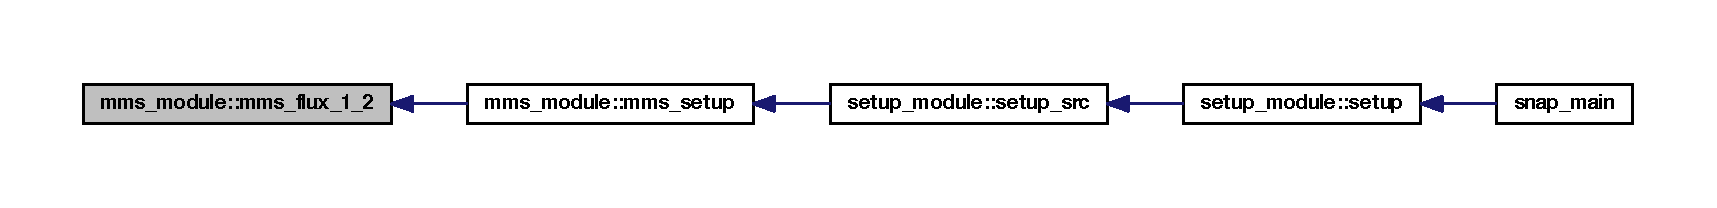
\includegraphics[width=350pt]{classmms__module_a8ed588a3dafe93834940e9df3460969b_icgraph}
\end{center}
\end{figure}


\hypertarget{classmms__module_af6e2504f62297dcb69f3939549152fef}{\index{mms\-\_\-module@{mms\-\_\-module}!mms\-\_\-setup@{mms\-\_\-setup}}
\index{mms\-\_\-setup@{mms\-\_\-setup}!mms_module@{mms\-\_\-module}}
\subsubsection[{mms\-\_\-setup}]{\setlength{\rightskip}{0pt plus 5cm}subroutine, public mms\-\_\-module\-::mms\-\_\-setup (
\begin{DoxyParamCaption}
\item[{integer(i\-\_\-knd), intent(out)}]{ierr, }
\item[{character(len=64), intent(out)}]{error}
\end{DoxyParamCaption}
)}}\label{classmms__module_af6e2504f62297dcb69f3939549152fef}


Definition at line 61 of file mms.\-f90.



Here is the call graph for this function\-:\nopagebreak
\begin{figure}[H]
\begin{center}
\leavevmode
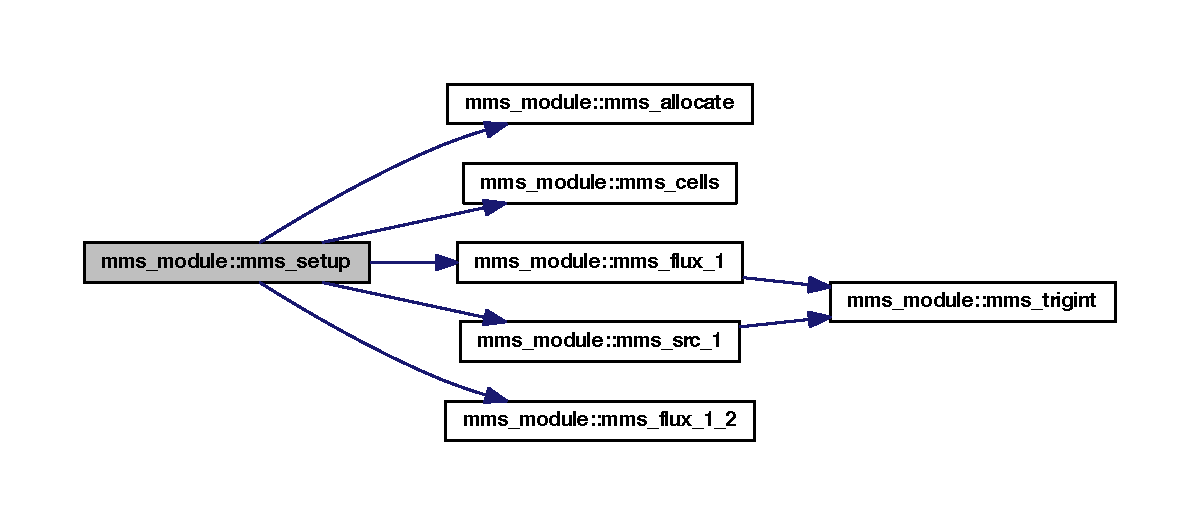
\includegraphics[width=350pt]{classmms__module_af6e2504f62297dcb69f3939549152fef_cgraph}
\end{center}
\end{figure}




Here is the caller graph for this function\-:\nopagebreak
\begin{figure}[H]
\begin{center}
\leavevmode
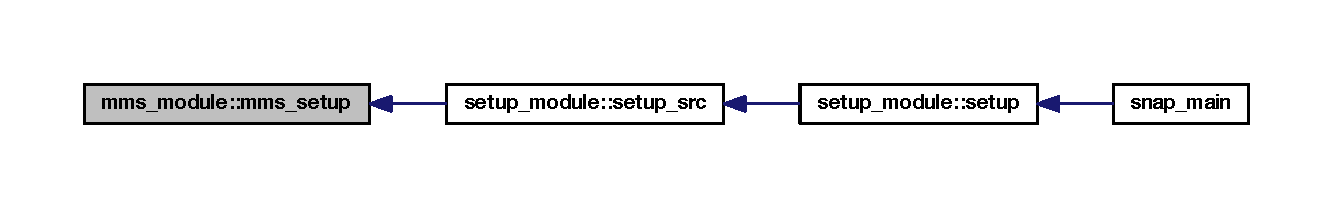
\includegraphics[width=350pt]{classmms__module_af6e2504f62297dcb69f3939549152fef_icgraph}
\end{center}
\end{figure}


\hypertarget{classmms__module_aa571bba8b81b30ec0d1560f2d6bd4e2a}{\index{mms\-\_\-module@{mms\-\_\-module}!mms\-\_\-src\-\_\-1@{mms\-\_\-src\-\_\-1}}
\index{mms\-\_\-src\-\_\-1@{mms\-\_\-src\-\_\-1}!mms_module@{mms\-\_\-module}}
\subsubsection[{mms\-\_\-src\-\_\-1}]{\setlength{\rightskip}{0pt plus 5cm}subroutine mms\-\_\-module\-::mms\-\_\-src\-\_\-1 (
\begin{DoxyParamCaption}
{}
\end{DoxyParamCaption}
)\hspace{0.3cm}{\ttfamily [private]}}}\label{classmms__module_aa571bba8b81b30ec0d1560f2d6bd4e2a}


Definition at line 352 of file mms.\-f90.



Here is the call graph for this function\-:\nopagebreak
\begin{figure}[H]
\begin{center}
\leavevmode
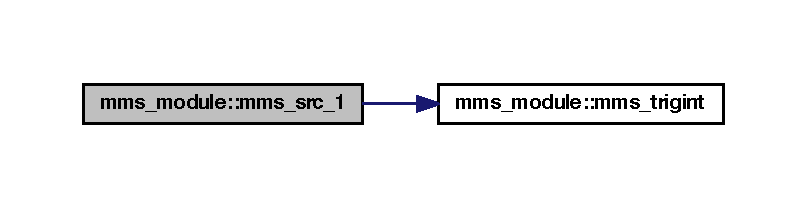
\includegraphics[width=350pt]{classmms__module_aa571bba8b81b30ec0d1560f2d6bd4e2a_cgraph}
\end{center}
\end{figure}




Here is the caller graph for this function\-:\nopagebreak
\begin{figure}[H]
\begin{center}
\leavevmode
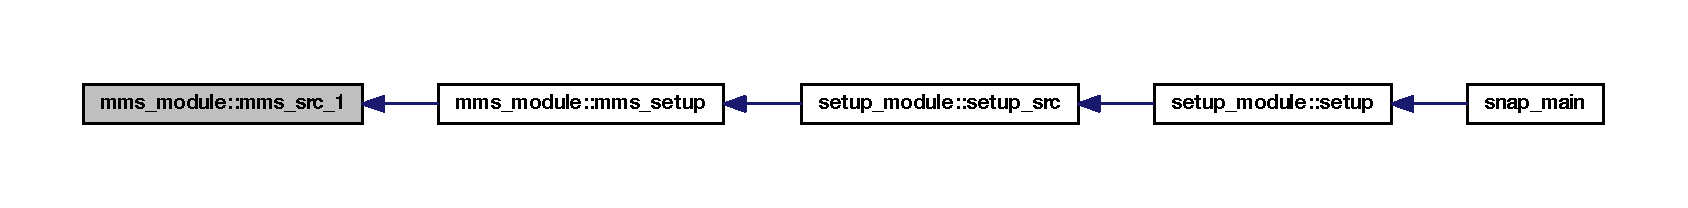
\includegraphics[width=350pt]{classmms__module_aa571bba8b81b30ec0d1560f2d6bd4e2a_icgraph}
\end{center}
\end{figure}


\hypertarget{classmms__module_a92298f4f6f9a03d54169aee15197f591}{\index{mms\-\_\-module@{mms\-\_\-module}!mms\-\_\-trigint@{mms\-\_\-trigint}}
\index{mms\-\_\-trigint@{mms\-\_\-trigint}!mms_module@{mms\-\_\-module}}
\subsubsection[{mms\-\_\-trigint}]{\setlength{\rightskip}{0pt plus 5cm}subroutine mms\-\_\-module\-::mms\-\_\-trigint (
\begin{DoxyParamCaption}
\item[{character(len=3), intent(in)}]{trig, }
\item[{integer(i\-\_\-knd), intent(in)}]{lc, }
\item[{real(r\-\_\-knd), intent(in)}]{d, }
\item[{real(r\-\_\-knd), intent(in)}]{del, }
\item[{real(r\-\_\-knd), dimension(lc+1), intent(in)}]{cb, }
\item[{real(r\-\_\-knd), dimension(lc), intent(out)}]{fn}
\end{DoxyParamCaption}
)\hspace{0.3cm}{\ttfamily [private]}}}\label{classmms__module_a92298f4f6f9a03d54169aee15197f591}


Definition at line 302 of file mms.\-f90.



Here is the caller graph for this function\-:\nopagebreak
\begin{figure}[H]
\begin{center}
\leavevmode
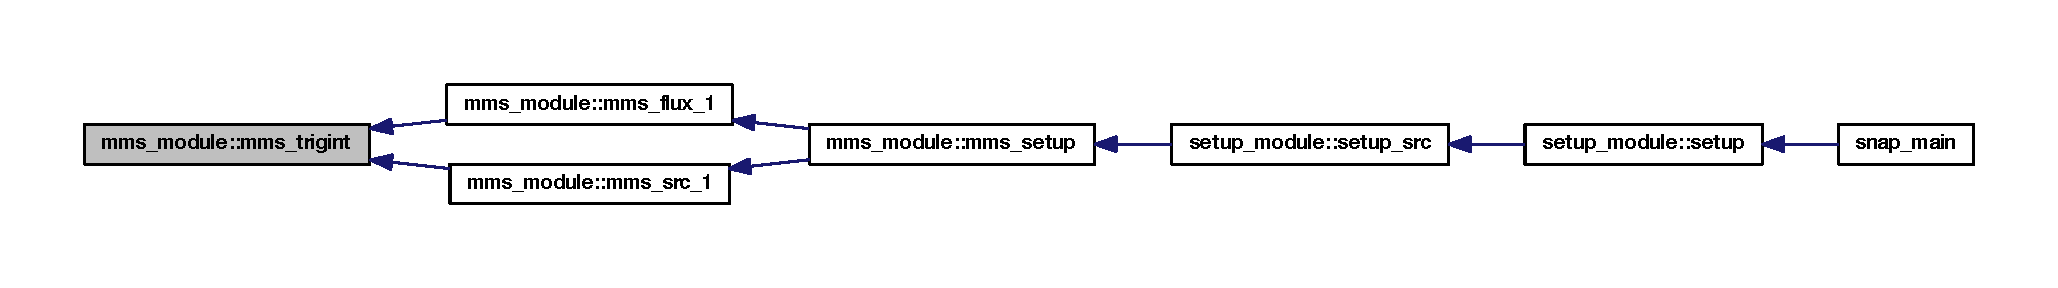
\includegraphics[width=350pt]{classmms__module_a92298f4f6f9a03d54169aee15197f591_icgraph}
\end{center}
\end{figure}


\hypertarget{classmms__module_a37e1faf94ca3526af48c3e8efc1d332a}{\index{mms\-\_\-module@{mms\-\_\-module}!mms\-\_\-verify\-\_\-1@{mms\-\_\-verify\-\_\-1}}
\index{mms\-\_\-verify\-\_\-1@{mms\-\_\-verify\-\_\-1}!mms_module@{mms\-\_\-module}}
\subsubsection[{mms\-\_\-verify\-\_\-1}]{\setlength{\rightskip}{0pt plus 5cm}subroutine, public mms\-\_\-module\-::mms\-\_\-verify\-\_\-1 (
\begin{DoxyParamCaption}
\item[{real(r\-\_\-knd), dimension(nx,ny,nz,ng), intent(in)}]{flux}
\end{DoxyParamCaption}
)}}\label{classmms__module_a37e1faf94ca3526af48c3e8efc1d332a}


Definition at line 507 of file mms.\-f90.



Here is the caller graph for this function\-:\nopagebreak
\begin{figure}[H]
\begin{center}
\leavevmode
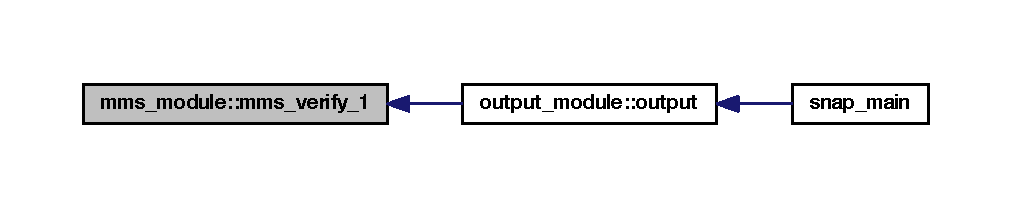
\includegraphics[width=350pt]{classmms__module_a37e1faf94ca3526af48c3e8efc1d332a_icgraph}
\end{center}
\end{figure}




\subsection{Member Data Documentation}
\hypertarget{classmms__module_a874f8531253686519c7dd40848edbc00}{\index{mms\-\_\-module@{mms\-\_\-module}!a@{a}}
\index{a@{a}!mms_module@{mms\-\_\-module}}
\subsubsection[{a}]{\setlength{\rightskip}{0pt plus 5cm}real(r\-\_\-knd) mms\-\_\-module\-::a\hspace{0.3cm}{\ttfamily [private]}}}\label{classmms__module_a874f8531253686519c7dd40848edbc00}


Definition at line 49 of file mms.\-f90.

\hypertarget{classmms__module_adb85ae57ca25aea5f2e91f7df6d53dc1}{\index{mms\-\_\-module@{mms\-\_\-module}!b@{b}}
\index{b@{b}!mms_module@{mms\-\_\-module}}
\subsubsection[{b}]{\setlength{\rightskip}{0pt plus 5cm}real(r\-\_\-knd) mms\-\_\-module\-::b\hspace{0.3cm}{\ttfamily [private]}}}\label{classmms__module_adb85ae57ca25aea5f2e91f7df6d53dc1}


Definition at line 49 of file mms.\-f90.

\hypertarget{classmms__module_a6bd089f9df8ee45c901b6830eca017f6}{\index{mms\-\_\-module@{mms\-\_\-module}!c@{c}}
\index{c@{c}!mms_module@{mms\-\_\-module}}
\subsubsection[{c}]{\setlength{\rightskip}{0pt plus 5cm}real(r\-\_\-knd) mms\-\_\-module\-::c\hspace{0.3cm}{\ttfamily [private]}}}\label{classmms__module_a6bd089f9df8ee45c901b6830eca017f6}


Definition at line 49 of file mms.\-f90.

\hypertarget{classmms__module_aaca218de11850fada15be6a3bbeb5159}{\index{mms\-\_\-module@{mms\-\_\-module}!ib@{ib}}
\index{ib@{ib}!mms_module@{mms\-\_\-module}}
\subsubsection[{ib}]{\setlength{\rightskip}{0pt plus 5cm}real(r\-\_\-knd), dimension(\-:), allocatable mms\-\_\-module\-::ib\hspace{0.3cm}{\ttfamily [private]}}}\label{classmms__module_aaca218de11850fada15be6a3bbeb5159}


Definition at line 51 of file mms.\-f90.

\hypertarget{classmms__module_a53a60661b3d933e48dbf0a926a4b010c}{\index{mms\-\_\-module@{mms\-\_\-module}!jb@{jb}}
\index{jb@{jb}!mms_module@{mms\-\_\-module}}
\subsubsection[{jb}]{\setlength{\rightskip}{0pt plus 5cm}real(r\-\_\-knd), dimension(\-:), allocatable mms\-\_\-module\-::jb\hspace{0.3cm}{\ttfamily [private]}}}\label{classmms__module_a53a60661b3d933e48dbf0a926a4b010c}


Definition at line 51 of file mms.\-f90.

\hypertarget{classmms__module_a634bb1d1d1405007f6bec01e8b6d9b85}{\index{mms\-\_\-module@{mms\-\_\-module}!kb@{kb}}
\index{kb@{kb}!mms_module@{mms\-\_\-module}}
\subsubsection[{kb}]{\setlength{\rightskip}{0pt plus 5cm}real(r\-\_\-knd), dimension(\-:), allocatable mms\-\_\-module\-::kb\hspace{0.3cm}{\ttfamily [private]}}}\label{classmms__module_a634bb1d1d1405007f6bec01e8b6d9b85}


Definition at line 51 of file mms.\-f90.

\hypertarget{classmms__module_a20157f9a49b1c0b449c340b7b1a63791}{\index{mms\-\_\-module@{mms\-\_\-module}!ref\-\_\-flux@{ref\-\_\-flux}}
\index{ref\-\_\-flux@{ref\-\_\-flux}!mms_module@{mms\-\_\-module}}
\subsubsection[{ref\-\_\-flux}]{\setlength{\rightskip}{0pt plus 5cm}real(r\-\_\-knd), dimension(\-:,\-:,\-:,\-:), allocatable, public mms\-\_\-module\-::ref\-\_\-flux}}\label{classmms__module_a20157f9a49b1c0b449c340b7b1a63791}


Definition at line 53 of file mms.\-f90.

\hypertarget{classmms__module_aaa592b5b9f1591e2a34df390563b0c56}{\index{mms\-\_\-module@{mms\-\_\-module}!ref\-\_\-fluxm@{ref\-\_\-fluxm}}
\index{ref\-\_\-fluxm@{ref\-\_\-fluxm}!mms_module@{mms\-\_\-module}}
\subsubsection[{ref\-\_\-fluxm}]{\setlength{\rightskip}{0pt plus 5cm}real(r\-\_\-knd), dimension(\-:,\-:,\-:,\-:,\-:), allocatable, public mms\-\_\-module\-::ref\-\_\-fluxm}}\label{classmms__module_aaa592b5b9f1591e2a34df390563b0c56}


Definition at line 55 of file mms.\-f90.



The documentation for this module was generated from the following file\-:\begin{DoxyCompactItemize}
\item 
src/\hyperlink{mms_8f90}{mms.\-f90}\end{DoxyCompactItemize}

\hypertarget{classoctsweep__module}{\section{octsweep\-\_\-module Module Reference}
\label{classoctsweep__module}\index{octsweep\-\_\-module@{octsweep\-\_\-module}}
}


This module controls the setup and calls for sweeping a single octant pair. It calls for the actual sweep logic depending on the spatial dimensionality of the problem.  


\subsection*{Public Member Functions}
\begin{DoxyCompactItemize}
\item 
subroutine, public \hyperlink{classoctsweep__module_af58dfb8973e3755aeeaa82bae73d2aef}{octsweep} (g, iop, jd, kd, jlo, jhi, jst, klo, khi, kst)
\end{DoxyCompactItemize}


\subsection{Detailed Description}
This module controls the setup and calls for sweeping a single octant pair. It calls for the actual sweep logic depending on the spatial dimensionality of the problem. 

Definition at line 11 of file octsweep.\-f90.



\subsection{Member Function/\-Subroutine Documentation}
\hypertarget{classoctsweep__module_af58dfb8973e3755aeeaa82bae73d2aef}{\index{octsweep\-\_\-module@{octsweep\-\_\-module}!octsweep@{octsweep}}
\index{octsweep@{octsweep}!octsweep_module@{octsweep\-\_\-module}}
\subsubsection[{octsweep}]{\setlength{\rightskip}{0pt plus 5cm}subroutine, public octsweep\-\_\-module\-::octsweep (
\begin{DoxyParamCaption}
\item[{integer(i\-\_\-knd), intent(in)}]{g, }
\item[{integer(i\-\_\-knd), intent(in)}]{iop, }
\item[{integer(i\-\_\-knd), intent(in)}]{jd, }
\item[{integer(i\-\_\-knd), intent(in)}]{kd, }
\item[{integer(i\-\_\-knd), intent(in)}]{jlo, }
\item[{integer(i\-\_\-knd), intent(in)}]{jhi, }
\item[{integer(i\-\_\-knd), intent(in)}]{jst, }
\item[{integer(i\-\_\-knd), intent(in)}]{klo, }
\item[{integer(i\-\_\-knd), intent(in)}]{khi, }
\item[{integer(i\-\_\-knd), intent(in)}]{kst}
\end{DoxyParamCaption}
)}}\label{classoctsweep__module_af58dfb8973e3755aeeaa82bae73d2aef}


Definition at line 38 of file octsweep.\-f90.



Here is the call graph for this function\-:\nopagebreak
\begin{figure}[H]
\begin{center}
\leavevmode
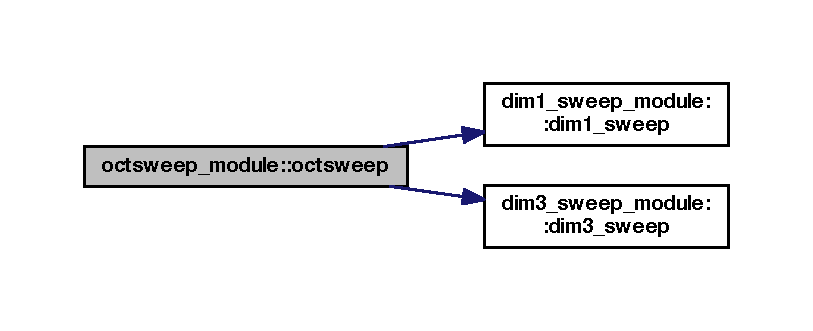
\includegraphics[width=350pt]{classoctsweep__module_af58dfb8973e3755aeeaa82bae73d2aef_cgraph}
\end{center}
\end{figure}




Here is the caller graph for this function\-:\nopagebreak
\begin{figure}[H]
\begin{center}
\leavevmode
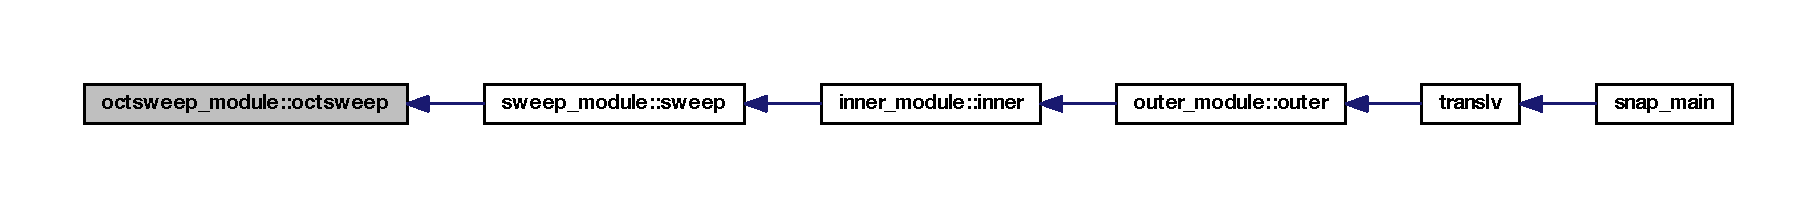
\includegraphics[width=350pt]{classoctsweep__module_af58dfb8973e3755aeeaa82bae73d2aef_icgraph}
\end{center}
\end{figure}




The documentation for this module was generated from the following file\-:\begin{DoxyCompactItemize}
\item 
src/\hyperlink{octsweep_8f90}{octsweep.\-f90}\end{DoxyCompactItemize}

\hypertarget{classouter__module}{\section{outer\-\_\-module Module Reference}
\label{classouter__module}\index{outer\-\_\-module@{outer\-\_\-module}}
}
\subsection*{Public Member Functions}
\begin{DoxyCompactItemize}
\item 
subroutine, public \hyperlink{classouter__module_a2deee1d5431094eb8d9c17c09666a844}{outer} (sum\-\_\-iits)
\end{DoxyCompactItemize}
\subsection*{Private Member Functions}
\begin{DoxyCompactItemize}
\item 
subroutine \hyperlink{classouter__module_acdd24e16ca56ddbc18ced7fca3073920}{otr\-\_\-src}
\item 
subroutine \hyperlink{classouter__module_a768cdc8f62d3f03c48810935e0c7d7a6}{otr\-\_\-src\-\_\-scat} (q, cs, map, f, fm)
\item 
subroutine \hyperlink{classouter__module_a084cd5d518ac2e6f60b82677797381ca}{otr\-\_\-conv}
\end{DoxyCompactItemize}


\subsection{Detailed Description}


Definition at line 1 of file outer.\-f90.



\subsection{Member Function/\-Subroutine Documentation}
\hypertarget{classouter__module_a084cd5d518ac2e6f60b82677797381ca}{\index{outer\-\_\-module@{outer\-\_\-module}!otr\-\_\-conv@{otr\-\_\-conv}}
\index{otr\-\_\-conv@{otr\-\_\-conv}!outer_module@{outer\-\_\-module}}
\subsubsection[{otr\-\_\-conv}]{\setlength{\rightskip}{0pt plus 5cm}subroutine outer\-\_\-module\-::otr\-\_\-conv (
\begin{DoxyParamCaption}
{}
\end{DoxyParamCaption}
)\hspace{0.3cm}{\ttfamily [private]}}}\label{classouter__module_a084cd5d518ac2e6f60b82677797381ca}


Definition at line 218 of file outer.\-f90.



Here is the caller graph for this function\-:\nopagebreak
\begin{figure}[H]
\begin{center}
\leavevmode
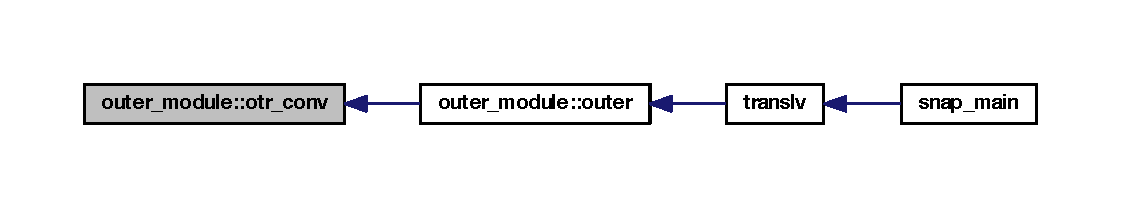
\includegraphics[width=350pt]{classouter__module_a084cd5d518ac2e6f60b82677797381ca_icgraph}
\end{center}
\end{figure}


\hypertarget{classouter__module_acdd24e16ca56ddbc18ced7fca3073920}{\index{outer\-\_\-module@{outer\-\_\-module}!otr\-\_\-src@{otr\-\_\-src}}
\index{otr\-\_\-src@{otr\-\_\-src}!outer_module@{outer\-\_\-module}}
\subsubsection[{otr\-\_\-src}]{\setlength{\rightskip}{0pt plus 5cm}subroutine outer\-\_\-module\-::otr\-\_\-src (
\begin{DoxyParamCaption}
{}
\end{DoxyParamCaption}
)\hspace{0.3cm}{\ttfamily [private]}}}\label{classouter__module_acdd24e16ca56ddbc18ced7fca3073920}


Definition at line 119 of file outer.\-f90.



Here is the call graph for this function\-:\nopagebreak
\begin{figure}[H]
\begin{center}
\leavevmode
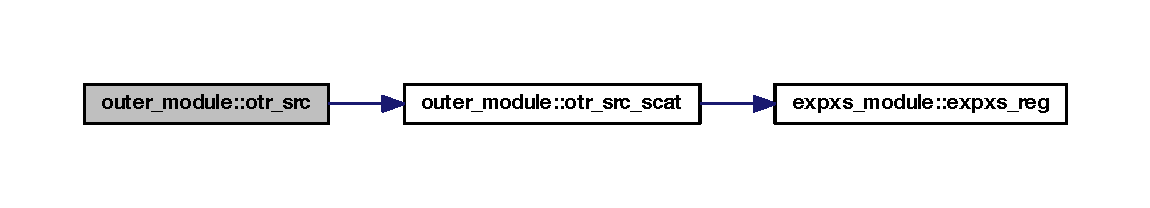
\includegraphics[width=350pt]{classouter__module_acdd24e16ca56ddbc18ced7fca3073920_cgraph}
\end{center}
\end{figure}




Here is the caller graph for this function\-:\nopagebreak
\begin{figure}[H]
\begin{center}
\leavevmode
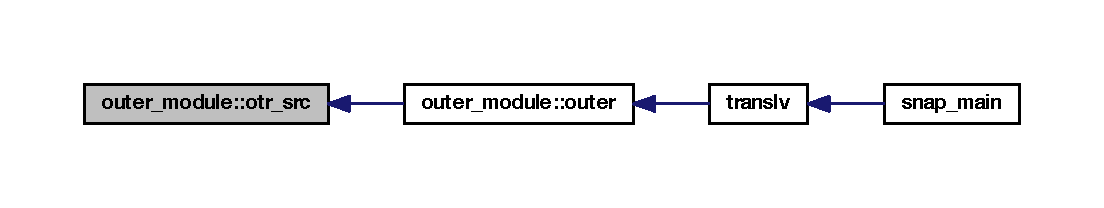
\includegraphics[width=350pt]{classouter__module_acdd24e16ca56ddbc18ced7fca3073920_icgraph}
\end{center}
\end{figure}


\hypertarget{classouter__module_a768cdc8f62d3f03c48810935e0c7d7a6}{\index{outer\-\_\-module@{outer\-\_\-module}!otr\-\_\-src\-\_\-scat@{otr\-\_\-src\-\_\-scat}}
\index{otr\-\_\-src\-\_\-scat@{otr\-\_\-src\-\_\-scat}!outer_module@{outer\-\_\-module}}
\subsubsection[{otr\-\_\-src\-\_\-scat}]{\setlength{\rightskip}{0pt plus 5cm}subroutine outer\-\_\-module\-::otr\-\_\-src\-\_\-scat (
\begin{DoxyParamCaption}
\item[{real(r\-\_\-knd), dimension(cmom,nx,ny,nz), intent(inout)}]{q, }
\item[{real(r\-\_\-knd), dimension(nmat,nmom), intent(in)}]{cs, }
\item[{integer(i\-\_\-knd), dimension(nx,ny,nz), intent(in)}]{map, }
\item[{real(r\-\_\-knd), dimension(nx,ny,nz), intent(in)}]{f, }
\item[{real(r\-\_\-knd), dimension(cmom-\/1,nx,ny,nz), intent(in)}]{fm}
\end{DoxyParamCaption}
)\hspace{0.3cm}{\ttfamily [private]}}}\label{classouter__module_a768cdc8f62d3f03c48810935e0c7d7a6}


Definition at line 162 of file outer.\-f90.



Here is the call graph for this function\-:\nopagebreak
\begin{figure}[H]
\begin{center}
\leavevmode
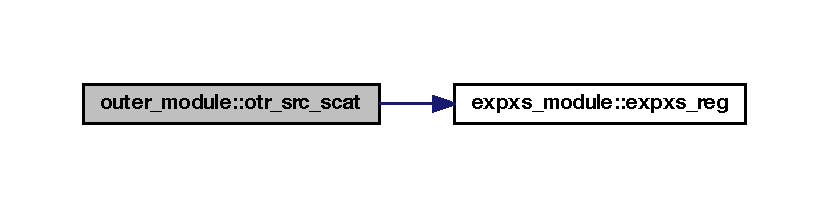
\includegraphics[width=350pt]{classouter__module_a768cdc8f62d3f03c48810935e0c7d7a6_cgraph}
\end{center}
\end{figure}




Here is the caller graph for this function\-:\nopagebreak
\begin{figure}[H]
\begin{center}
\leavevmode
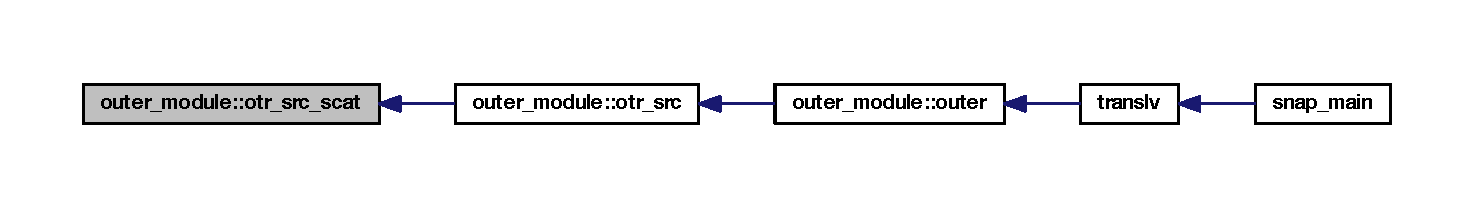
\includegraphics[width=350pt]{classouter__module_a768cdc8f62d3f03c48810935e0c7d7a6_icgraph}
\end{center}
\end{figure}


\hypertarget{classouter__module_a2deee1d5431094eb8d9c17c09666a844}{\index{outer\-\_\-module@{outer\-\_\-module}!outer@{outer}}
\index{outer@{outer}!outer_module@{outer\-\_\-module}}
\subsubsection[{outer}]{\setlength{\rightskip}{0pt plus 5cm}subroutine, public outer\-\_\-module\-::outer (
\begin{DoxyParamCaption}
\item[{integer(i\-\_\-knd), intent(out)}]{sum\-\_\-iits}
\end{DoxyParamCaption}
)}}\label{classouter__module_a2deee1d5431094eb8d9c17c09666a844}


Definition at line 43 of file outer.\-f90.



Here is the call graph for this function\-:\nopagebreak
\begin{figure}[H]
\begin{center}
\leavevmode
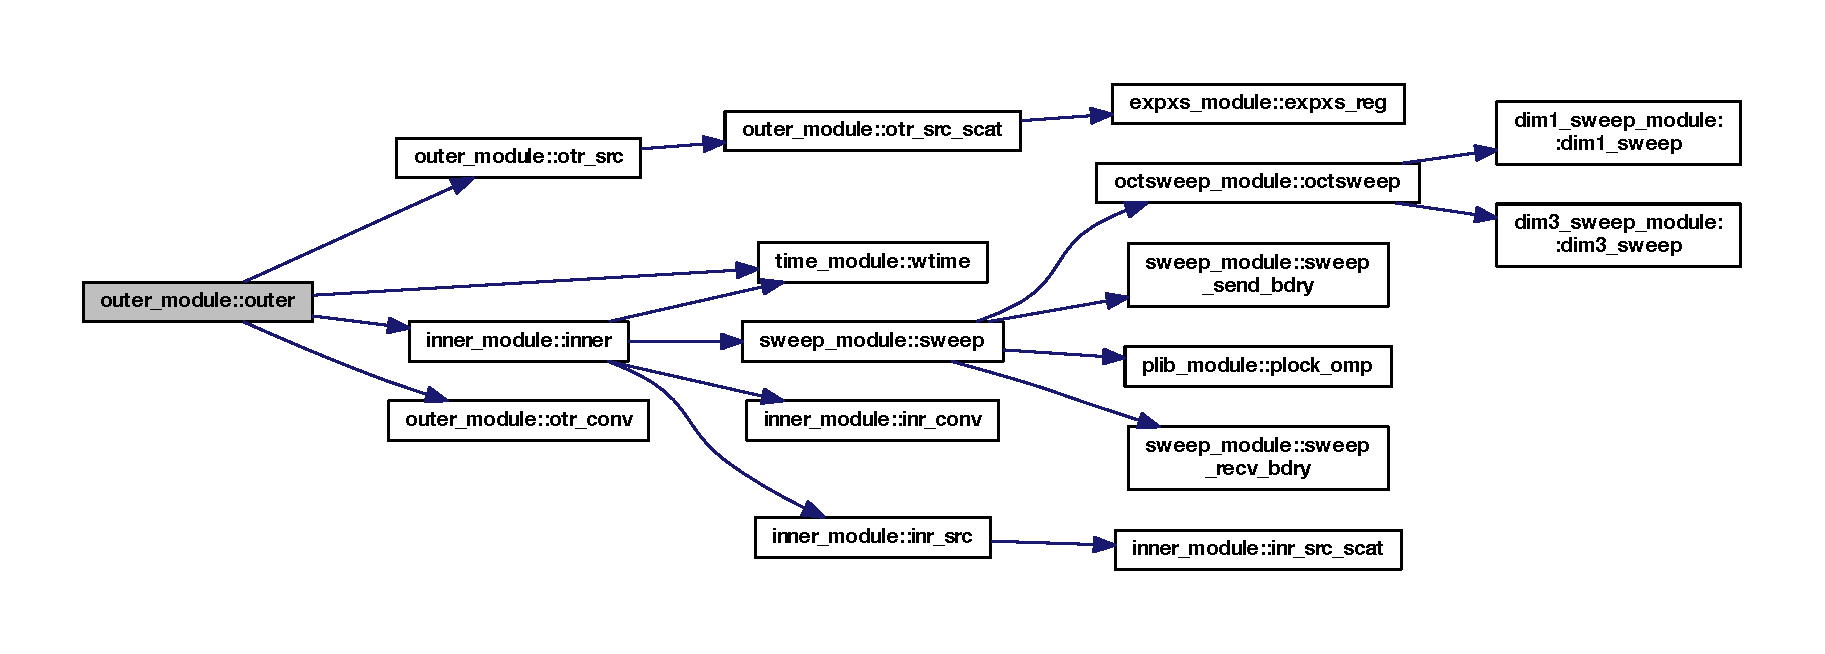
\includegraphics[width=350pt]{classouter__module_a2deee1d5431094eb8d9c17c09666a844_cgraph}
\end{center}
\end{figure}




Here is the caller graph for this function\-:\nopagebreak
\begin{figure}[H]
\begin{center}
\leavevmode
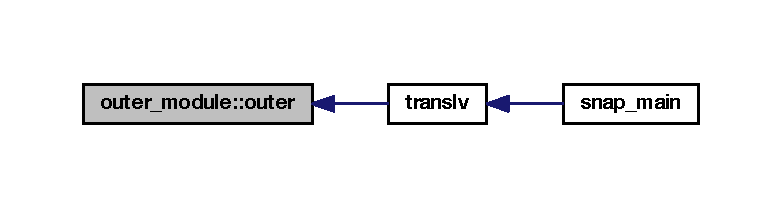
\includegraphics[width=350pt]{classouter__module_a2deee1d5431094eb8d9c17c09666a844_icgraph}
\end{center}
\end{figure}




The documentation for this module was generated from the following file\-:\begin{DoxyCompactItemize}
\item 
src/\hyperlink{outer_8f90}{outer.\-f90}\end{DoxyCompactItemize}

\hypertarget{classoutput__module}{\section{output\-\_\-module Module Reference}
\label{classoutput__module}\index{output\-\_\-module@{output\-\_\-module}}
}


This module controls final solution output.  


\subsection*{Public Member Functions}
\begin{DoxyCompactItemize}
\item 
subroutine, public \hyperlink{classoutput__module_ac6eaa7844cc1fbf453e8774182ad6edf}{output}
\end{DoxyCompactItemize}
\subsection*{Private Member Functions}
\begin{DoxyCompactItemize}
\item 
subroutine \hyperlink{classoutput__module_a4cdf2d1c235c931cf2366e20987d7f98}{output\-\_\-send} (mtag, fprnt)
\item 
subroutine \hyperlink{classoutput__module_a3eaf5aa5b2a2809f84916c6df3d6945c}{output\-\_\-recv} (mtag, proc, fprnt)
\item 
subroutine \hyperlink{classoutput__module_aab79ee63006002c5b231a79051640d97}{output\-\_\-flux\-\_\-file} (klb, kub)
\end{DoxyCompactItemize}


\subsection{Detailed Description}
This module controls final solution output. 

Definition at line 9 of file output.\-f90.



\subsection{Member Function/\-Subroutine Documentation}
\hypertarget{classoutput__module_ac6eaa7844cc1fbf453e8774182ad6edf}{\index{output\-\_\-module@{output\-\_\-module}!output@{output}}
\index{output@{output}!output_module@{output\-\_\-module}}
\subsubsection[{output}]{\setlength{\rightskip}{0pt plus 5cm}subroutine, public output\-\_\-module\-::output (
\begin{DoxyParamCaption}
{}
\end{DoxyParamCaption}
)}}\label{classoutput__module_ac6eaa7844cc1fbf453e8774182ad6edf}


Definition at line 42 of file output.\-f90.



Here is the call graph for this function\-:\nopagebreak
\begin{figure}[H]
\begin{center}
\leavevmode
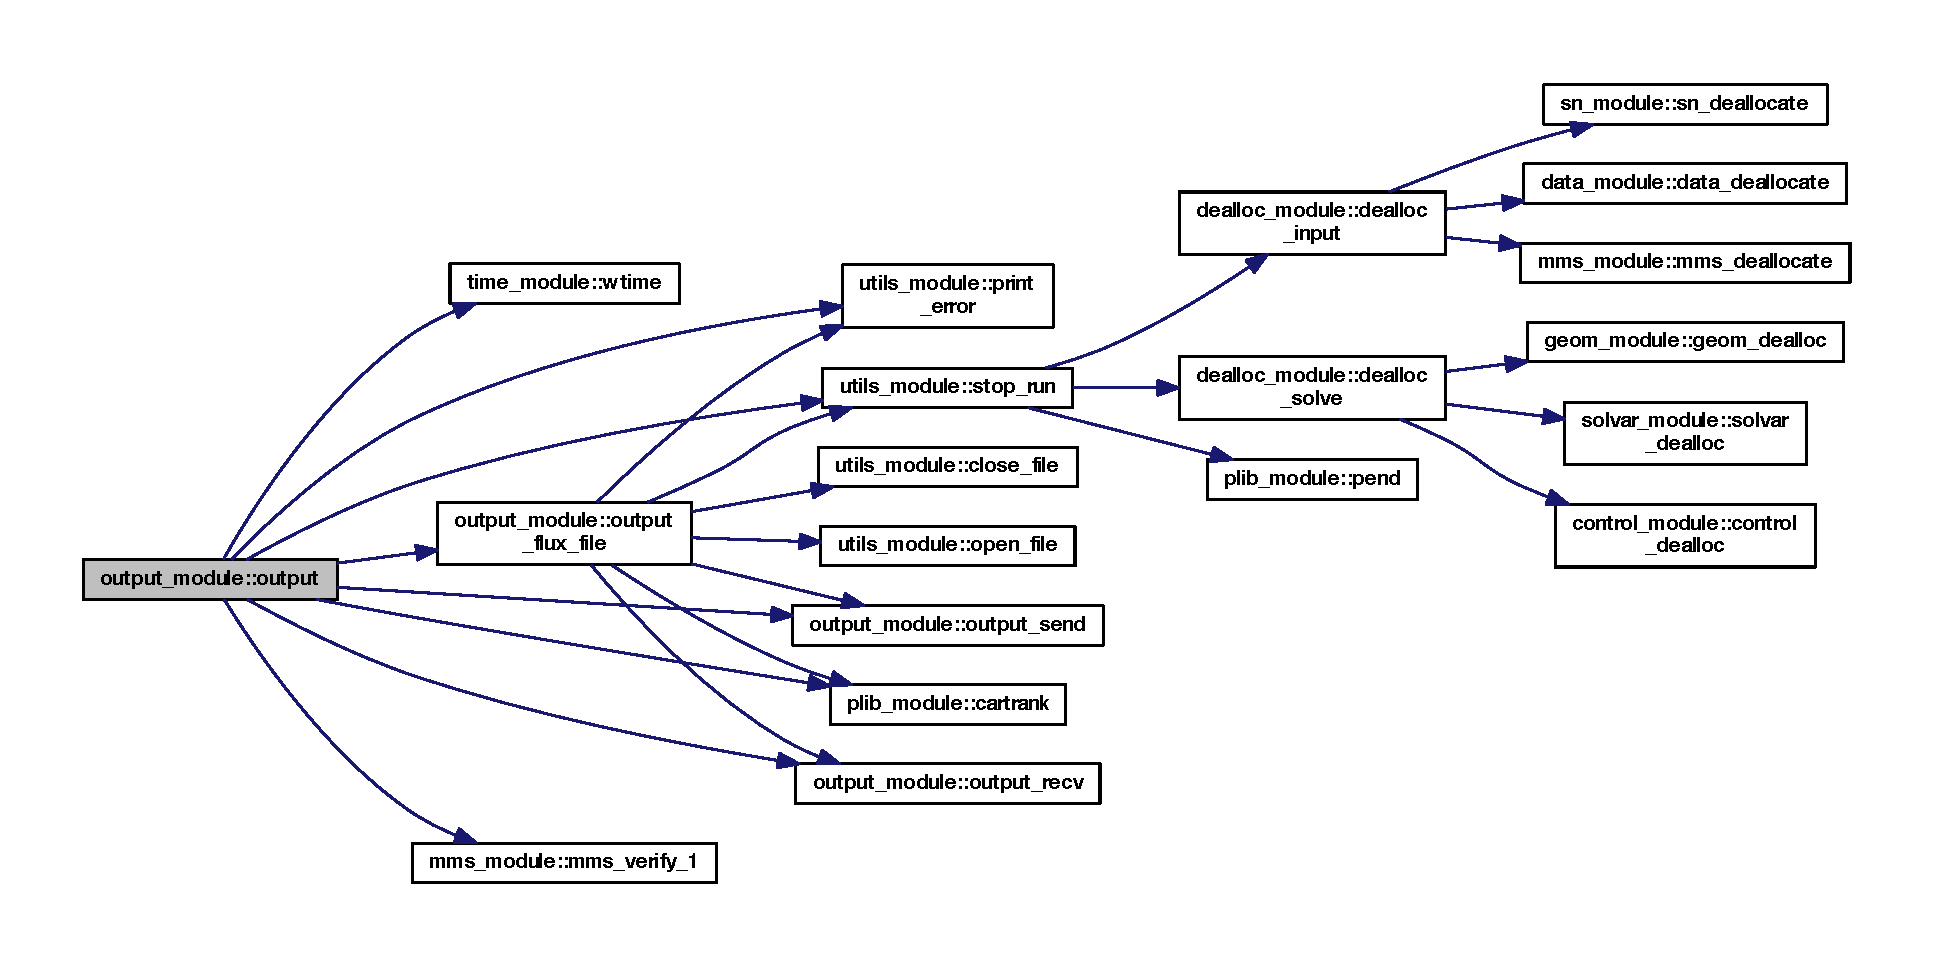
\includegraphics[width=350pt]{classoutput__module_ac6eaa7844cc1fbf453e8774182ad6edf_cgraph}
\end{center}
\end{figure}




Here is the caller graph for this function\-:\nopagebreak
\begin{figure}[H]
\begin{center}
\leavevmode
\includegraphics[width=304pt]{classoutput__module_ac6eaa7844cc1fbf453e8774182ad6edf_icgraph}
\end{center}
\end{figure}


\hypertarget{classoutput__module_aab79ee63006002c5b231a79051640d97}{\index{output\-\_\-module@{output\-\_\-module}!output\-\_\-flux\-\_\-file@{output\-\_\-flux\-\_\-file}}
\index{output\-\_\-flux\-\_\-file@{output\-\_\-flux\-\_\-file}!output_module@{output\-\_\-module}}
\subsubsection[{output\-\_\-flux\-\_\-file}]{\setlength{\rightskip}{0pt plus 5cm}subroutine output\-\_\-module\-::output\-\_\-flux\-\_\-file (
\begin{DoxyParamCaption}
\item[{integer(i\-\_\-knd), intent(in)}]{klb, }
\item[{integer(i\-\_\-knd), intent(in)}]{kub}
\end{DoxyParamCaption}
)\hspace{0.3cm}{\ttfamily [private]}}}\label{classoutput__module_aab79ee63006002c5b231a79051640d97}


Definition at line 250 of file output.\-f90.



Here is the call graph for this function\-:\nopagebreak
\begin{figure}[H]
\begin{center}
\leavevmode
\includegraphics[width=350pt]{classoutput__module_aab79ee63006002c5b231a79051640d97_cgraph}
\end{center}
\end{figure}




Here is the caller graph for this function\-:\nopagebreak
\begin{figure}[H]
\begin{center}
\leavevmode
\includegraphics[width=350pt]{classoutput__module_aab79ee63006002c5b231a79051640d97_icgraph}
\end{center}
\end{figure}


\hypertarget{classoutput__module_a3eaf5aa5b2a2809f84916c6df3d6945c}{\index{output\-\_\-module@{output\-\_\-module}!output\-\_\-recv@{output\-\_\-recv}}
\index{output\-\_\-recv@{output\-\_\-recv}!output_module@{output\-\_\-module}}
\subsubsection[{output\-\_\-recv}]{\setlength{\rightskip}{0pt plus 5cm}subroutine output\-\_\-module\-::output\-\_\-recv (
\begin{DoxyParamCaption}
\item[{integer(i\-\_\-knd), intent(in)}]{mtag, }
\item[{integer(i\-\_\-knd), intent(in)}]{proc, }
\item[{real(r\-\_\-knd), dimension(nx,ny), intent(inout)}]{fprnt}
\end{DoxyParamCaption}
)\hspace{0.3cm}{\ttfamily [private]}}}\label{classoutput__module_a3eaf5aa5b2a2809f84916c6df3d6945c}


Definition at line 230 of file output.\-f90.



Here is the caller graph for this function\-:\nopagebreak
\begin{figure}[H]
\begin{center}
\leavevmode
\includegraphics[width=350pt]{classoutput__module_a3eaf5aa5b2a2809f84916c6df3d6945c_icgraph}
\end{center}
\end{figure}


\hypertarget{classoutput__module_a4cdf2d1c235c931cf2366e20987d7f98}{\index{output\-\_\-module@{output\-\_\-module}!output\-\_\-send@{output\-\_\-send}}
\index{output\-\_\-send@{output\-\_\-send}!output_module@{output\-\_\-module}}
\subsubsection[{output\-\_\-send}]{\setlength{\rightskip}{0pt plus 5cm}subroutine output\-\_\-module\-::output\-\_\-send (
\begin{DoxyParamCaption}
\item[{integer(i\-\_\-knd), intent(in)}]{mtag, }
\item[{real(r\-\_\-knd), dimension(nx,ny), intent(in)}]{fprnt}
\end{DoxyParamCaption}
)\hspace{0.3cm}{\ttfamily [private]}}}\label{classoutput__module_a4cdf2d1c235c931cf2366e20987d7f98}


Definition at line 210 of file output.\-f90.



Here is the caller graph for this function\-:\nopagebreak
\begin{figure}[H]
\begin{center}
\leavevmode
\includegraphics[width=350pt]{classoutput__module_a4cdf2d1c235c931cf2366e20987d7f98_icgraph}
\end{center}
\end{figure}




The documentation for this module was generated from the following file\-:\begin{DoxyCompactItemize}
\item 
src/\hyperlink{output_8f90}{output.\-f90}\end{DoxyCompactItemize}

\hypertarget{classplib__module}{\section{plib\-\_\-module Module Reference}
\label{classplib__module}\index{plib\-\_\-module@{plib\-\_\-module}}
}


This module contains the variables that control parallel decomposition and the subroutines for parallel environment setup. Only module that requires M\-P\-I library interaction except for \hyperlink{classtime__module}{time\-\_\-module} (M\-P\-I\-\_\-\-W\-T\-I\-M\-E).  


\subsection*{Data Types}
\begin{DoxyCompactItemize}
\item 
interface \hyperlink{interfaceplib__module_1_1bcast}{bcast}
\item 
interface \hyperlink{interfaceplib__module_1_1glmax}{glmax}
\item 
interface \hyperlink{interfaceplib__module_1_1glmin}{glmin}
\item 
interface \hyperlink{interfaceplib__module_1_1precv}{precv}
\item 
interface \hyperlink{interfaceplib__module_1_1psend}{psend}
\end{DoxyCompactItemize}
\subsection*{Public Member Functions}
\begin{DoxyCompactItemize}
\item 
subroutine \hyperlink{classplib__module_ae78d370a89bed99c28b886de57ae82d4}{pinit} (t1)
\item 
subroutine \hyperlink{classplib__module_a4e2a7d994f9e40d73d1f23d195421c88}{barrier} (comm)
\item 
subroutine \hyperlink{classplib__module_ae1bf2353a57332439fe7ceb97a6da009}{pcomm\-\_\-set}
\item 
subroutine \hyperlink{classplib__module_a8c714eb09fefa34353c52b163be411d7}{pend}
\item 
subroutine \hyperlink{classplib__module_a35e1e3d669c7e73e5481bc36b570907d}{glmax\-\_\-i} (value, comm)
\item 
subroutine \hyperlink{classplib__module_add45fae33090e71fdf132f7dcd8d154d}{glmax\-\_\-d} (value, comm)
\item 
subroutine \hyperlink{classplib__module_a1a64b5002b4f6b84133b4b0868fbc3b6}{glmax\-\_\-d\-\_\-1d} (value, dlen, comm)
\item 
subroutine \hyperlink{classplib__module_a1ab0a49a7d10568be52dc00a40bef825}{glmin\-\_\-i} (value, comm)
\item 
subroutine \hyperlink{classplib__module_a6e43b879b8deaee995c90a37345d1248}{glmin\-\_\-d} (value, comm)
\item 
subroutine \hyperlink{classplib__module_aa4dfae87ec1583a68a7fb3756bc4bbb1}{bcast\-\_\-i\-\_\-scalar} (value, comm, bproc)
\item 
subroutine \hyperlink{classplib__module_a5590b2a616e32329753421b685473604}{bcast\-\_\-i\-\_\-1d} (value, ilen, comm, bproc)
\item 
subroutine \hyperlink{classplib__module_a909b81966d60ec8340c1be57c6c5c073}{bcast\-\_\-d\-\_\-scalar} (value, comm, bproc)
\item 
subroutine \hyperlink{classplib__module_adbde05317e41d8723a54e5356627a27f}{bcast\-\_\-d\-\_\-1d} (value, dlen, comm, bproc)
\item 
subroutine \hyperlink{classplib__module_aece115e45bdb1399b9c969366b46404e}{psend\-\_\-d\-\_\-2d} (proc, myproc, d1, d2, value, comm, mtag)
\item 
subroutine \hyperlink{classplib__module_ac202cc24041fff90fa56158d02d64f70}{psend\-\_\-d\-\_\-3d} (proc, myproc, d1, d2, d3, value, comm, mtag)
\item 
subroutine \hyperlink{classplib__module_ac4722c07063b81f7b260132f16f5b17f}{precv\-\_\-d\-\_\-2d} (proc, myproc, d1, d2, value, comm, mtag)
\item 
subroutine \hyperlink{classplib__module_a4bb9d60a8dee39c7d1df606cb1ec48d1}{precv\-\_\-d\-\_\-3d} (proc, myproc, d1, d2, d3, value, comm, mtag)
\item 
subroutine \hyperlink{classplib__module_a31e3a1f18b78ea21eb4b76edcfc5352b}{cartrank} (coord, rank, comm)
\item 
subroutine \hyperlink{classplib__module_a5ad7e8ca3705ac070d1c9f1e63632153}{pinit\-\_\-omp} (ierr, error)
\item 
subroutine \hyperlink{classplib__module_af6742553d9df98f688231b8cd62cf190}{plock\-\_\-omp} (dowhat)
\item 
integer(i\-\_\-knd) function \hyperlink{classplib__module_a3b20a8eb56e03976578f415bf06ad72e}{thread\-\_\-num} ()
\end{DoxyCompactItemize}
\subsection*{Public Attributes}
\begin{DoxyCompactItemize}
\item 
integer(i\-\_\-knd) \hyperlink{classplib__module_a90134f6aac88ad1d7341e79cbf8426f1}{npey} = 1
\item 
integer(i\-\_\-knd) \hyperlink{classplib__module_ab827d3c46ffc494381bb0962d304561a}{npez} = 1
\item 
integer(i\-\_\-knd) \hyperlink{classplib__module_a0982ec611aac37b53db96a8266ff5c48}{ichunk} = 4
\item 
integer(i\-\_\-knd) \hyperlink{classplib__module_aac4e1911c67e39262528b4ebf471997d}{nthreads} = 1
\item 
integer(i\-\_\-knd) \hyperlink{classplib__module_a1fc540917e4a4c7e8677f74d81a58fc4}{nnested} = 0
\item 
integer(i\-\_\-knd), parameter \hyperlink{classplib__module_a4216863984e9df981d4a2d5a51020ce5}{root} = 0
\item 
integer(i\-\_\-knd), parameter \hyperlink{classplib__module_aa3f6bda8ab61c2acbdaf18afe105dbae}{g\-\_\-off} = 2$\ast$$\ast$14
\item 
integer(i\-\_\-knd) \hyperlink{classplib__module_ae01601bf17ba60fbd8ec154182186409}{nproc}
\item 
integer(i\-\_\-knd) \hyperlink{classplib__module_a20a10200b84fc53b3f9703d080eb4f41}{iproc}
\item 
integer(i\-\_\-knd) \hyperlink{classplib__module_a9819445413d7afeb56953bd9fe427854}{comm\-\_\-snap}
\item 
integer(i\-\_\-knd) \hyperlink{classplib__module_aa5bc6028743a524c4466548e276cb839}{comm\-\_\-space}
\item 
integer(i\-\_\-knd) \hyperlink{classplib__module_aa3b6e5883dfa628f71771e9e6ee3e722}{sproc}
\item 
integer(i\-\_\-knd) \hyperlink{classplib__module_af98dd05eb9d15041b5c783c6be090495}{ycomm}
\item 
integer(i\-\_\-knd) \hyperlink{classplib__module_aecf72186ecae9823c0bbe21808acb840}{zcomm}
\item 
integer(i\-\_\-knd) \hyperlink{classplib__module_a75e3d1fe13879374c5966909045b4670}{yproc}
\item 
integer(i\-\_\-knd) \hyperlink{classplib__module_abce2abcf8d84587f2d4a066fa1287d81}{zproc}
\item 
integer(i\-\_\-knd) \hyperlink{classplib__module_a95589a7523a49a05f8af1b39f7e75df8}{ylop}
\item 
integer(i\-\_\-knd) \hyperlink{classplib__module_a5520d897cd8da06d1815c1ec27010cf3}{yhip}
\item 
integer(i\-\_\-knd) \hyperlink{classplib__module_a3a7c2d7b52bbd28281bd1affd1d50bf1}{zlop}
\item 
integer(i\-\_\-knd) \hyperlink{classplib__module_ac18f767501ee98501fbf13da3185aae7}{zhip}
\item 
integer(i\-\_\-knd) \hyperlink{classplib__module_a704c693732d15c474f76b340e3b1c54f}{thread\-\_\-level}
\item 
integer(i\-\_\-knd) \hyperlink{classplib__module_a976973aed6846d0da2cc7fc29e0f0097}{thread\-\_\-single}
\item 
integer(i\-\_\-knd) \hyperlink{classplib__module_aaf61faf216e801843c4b8121eab84956}{thread\-\_\-funneled}
\item 
integer(i\-\_\-knd) \hyperlink{classplib__module_a117ac57a3b41c9fae508f8674fe45f0f}{thread\-\_\-serialized}
\item 
integer(i\-\_\-knd) \hyperlink{classplib__module_af4045f02bfdd6ce98120023046d4c1ca}{thread\-\_\-multiple}
\item 
integer(i\-\_\-knd) \hyperlink{classplib__module_aac421ecf4251867c4bff7045095d596c}{max\-\_\-threads}
\item 
integer(i\-\_\-knd) \hyperlink{classplib__module_a8238cefc81a445bee3e137bb94f75e91}{num\-\_\-grth}
\item 
logical(l\-\_\-knd) \hyperlink{classplib__module_acacb5f9f63dcc742ef176b99534fe626}{firsty}
\item 
logical(l\-\_\-knd) \hyperlink{classplib__module_ac8204e5b33211c1fe40e991a11d63f95}{lasty}
\item 
logical(l\-\_\-knd) \hyperlink{classplib__module_a2d791ed6cdd38a29604dcb99a7a556fe}{firstz}
\item 
logical(l\-\_\-knd) \hyperlink{classplib__module_a5d6addca95cdb6299949d278355bed3b}{lastz}
\item 
logical(l\-\_\-knd) \hyperlink{classplib__module_a68a4ebbe262904bf323f37f2e97ee5f2}{do\-\_\-nested}
\item 
integer(omp\-\_\-lock\-\_\-kind) \hyperlink{classplib__module_a3f4964cd381feb76e21407e3b96915c9}{lock}
\end{DoxyCompactItemize}


\subsection{Detailed Description}
This module contains the variables that control parallel decomposition and the subroutines for parallel environment setup. Only module that requires M\-P\-I library interaction except for \hyperlink{classtime__module}{time\-\_\-module} (M\-P\-I\-\_\-\-W\-T\-I\-M\-E). 

Definition at line 11 of file plib.\-f90.



\subsection{Member Function/\-Subroutine Documentation}
\hypertarget{classplib__module_a4e2a7d994f9e40d73d1f23d195421c88}{\index{plib\-\_\-module@{plib\-\_\-module}!barrier@{barrier}}
\index{barrier@{barrier}!plib_module@{plib\-\_\-module}}
\subsubsection[{barrier}]{\setlength{\rightskip}{0pt plus 5cm}subroutine plib\-\_\-module\-::barrier (
\begin{DoxyParamCaption}
\item[{integer(i\-\_\-knd), intent(in)}]{comm}
\end{DoxyParamCaption}
)}}\label{classplib__module_a4e2a7d994f9e40d73d1f23d195421c88}


Definition at line 175 of file plib.\-f90.



Here is the caller graph for this function\-:\nopagebreak
\begin{figure}[H]
\begin{center}
\leavevmode
\includegraphics[width=350pt]{classplib__module_a4e2a7d994f9e40d73d1f23d195421c88_icgraph}
\end{center}
\end{figure}


\hypertarget{classplib__module_adbde05317e41d8723a54e5356627a27f}{\index{plib\-\_\-module@{plib\-\_\-module}!bcast\-\_\-d\-\_\-1d@{bcast\-\_\-d\-\_\-1d}}
\index{bcast\-\_\-d\-\_\-1d@{bcast\-\_\-d\-\_\-1d}!plib_module@{plib\-\_\-module}}
\subsubsection[{bcast\-\_\-d\-\_\-1d}]{\setlength{\rightskip}{0pt plus 5cm}subroutine plib\-\_\-module\-::bcast\-\_\-d\-\_\-1d (
\begin{DoxyParamCaption}
\item[{real(r\-\_\-knd), dimension(dlen), intent(inout)}]{value, }
\item[{integer(i\-\_\-knd), intent(in)}]{dlen, }
\item[{integer(i\-\_\-knd), intent(in)}]{comm, }
\item[{integer(i\-\_\-knd), intent(in)}]{bproc}
\end{DoxyParamCaption}
)}}\label{classplib__module_adbde05317e41d8723a54e5356627a27f}


Definition at line 557 of file plib.\-f90.

\hypertarget{classplib__module_a909b81966d60ec8340c1be57c6c5c073}{\index{plib\-\_\-module@{plib\-\_\-module}!bcast\-\_\-d\-\_\-scalar@{bcast\-\_\-d\-\_\-scalar}}
\index{bcast\-\_\-d\-\_\-scalar@{bcast\-\_\-d\-\_\-scalar}!plib_module@{plib\-\_\-module}}
\subsubsection[{bcast\-\_\-d\-\_\-scalar}]{\setlength{\rightskip}{0pt plus 5cm}subroutine plib\-\_\-module\-::bcast\-\_\-d\-\_\-scalar (
\begin{DoxyParamCaption}
\item[{real(r\-\_\-knd), intent(inout)}]{value, }
\item[{integer(i\-\_\-knd), intent(in)}]{comm, }
\item[{integer(i\-\_\-knd), intent(in)}]{bproc}
\end{DoxyParamCaption}
)}}\label{classplib__module_a909b81966d60ec8340c1be57c6c5c073}


Definition at line 527 of file plib.\-f90.

\hypertarget{classplib__module_a5590b2a616e32329753421b685473604}{\index{plib\-\_\-module@{plib\-\_\-module}!bcast\-\_\-i\-\_\-1d@{bcast\-\_\-i\-\_\-1d}}
\index{bcast\-\_\-i\-\_\-1d@{bcast\-\_\-i\-\_\-1d}!plib_module@{plib\-\_\-module}}
\subsubsection[{bcast\-\_\-i\-\_\-1d}]{\setlength{\rightskip}{0pt plus 5cm}subroutine plib\-\_\-module\-::bcast\-\_\-i\-\_\-1d (
\begin{DoxyParamCaption}
\item[{integer(i\-\_\-knd), dimension(ilen), intent(inout)}]{value, }
\item[{integer(i\-\_\-knd), intent(in)}]{ilen, }
\item[{integer(i\-\_\-knd), intent(in)}]{comm, }
\item[{integer(i\-\_\-knd), intent(in)}]{bproc}
\end{DoxyParamCaption}
)}}\label{classplib__module_a5590b2a616e32329753421b685473604}


Definition at line 496 of file plib.\-f90.

\hypertarget{classplib__module_aa4dfae87ec1583a68a7fb3756bc4bbb1}{\index{plib\-\_\-module@{plib\-\_\-module}!bcast\-\_\-i\-\_\-scalar@{bcast\-\_\-i\-\_\-scalar}}
\index{bcast\-\_\-i\-\_\-scalar@{bcast\-\_\-i\-\_\-scalar}!plib_module@{plib\-\_\-module}}
\subsubsection[{bcast\-\_\-i\-\_\-scalar}]{\setlength{\rightskip}{0pt plus 5cm}subroutine plib\-\_\-module\-::bcast\-\_\-i\-\_\-scalar (
\begin{DoxyParamCaption}
\item[{integer(i\-\_\-knd), intent(inout)}]{value, }
\item[{integer(i\-\_\-knd), intent(in)}]{comm, }
\item[{integer(i\-\_\-knd), intent(in)}]{bproc}
\end{DoxyParamCaption}
)}}\label{classplib__module_aa4dfae87ec1583a68a7fb3756bc4bbb1}


Definition at line 466 of file plib.\-f90.

\hypertarget{classplib__module_a31e3a1f18b78ea21eb4b76edcfc5352b}{\index{plib\-\_\-module@{plib\-\_\-module}!cartrank@{cartrank}}
\index{cartrank@{cartrank}!plib_module@{plib\-\_\-module}}
\subsubsection[{cartrank}]{\setlength{\rightskip}{0pt plus 5cm}subroutine plib\-\_\-module\-::cartrank (
\begin{DoxyParamCaption}
\item[{integer(i\-\_\-knd), dimension(2), intent(in)}]{coord, }
\item[{integer(i\-\_\-knd), intent(out)}]{rank, }
\item[{integer(i\-\_\-knd), intent(in)}]{comm}
\end{DoxyParamCaption}
)}}\label{classplib__module_a31e3a1f18b78ea21eb4b76edcfc5352b}


Definition at line 712 of file plib.\-f90.



Here is the caller graph for this function\-:\nopagebreak
\begin{figure}[H]
\begin{center}
\leavevmode
\includegraphics[width=350pt]{classplib__module_a31e3a1f18b78ea21eb4b76edcfc5352b_icgraph}
\end{center}
\end{figure}


\hypertarget{classplib__module_add45fae33090e71fdf132f7dcd8d154d}{\index{plib\-\_\-module@{plib\-\_\-module}!glmax\-\_\-d@{glmax\-\_\-d}}
\index{glmax\-\_\-d@{glmax\-\_\-d}!plib_module@{plib\-\_\-module}}
\subsubsection[{glmax\-\_\-d}]{\setlength{\rightskip}{0pt plus 5cm}subroutine plib\-\_\-module\-::glmax\-\_\-d (
\begin{DoxyParamCaption}
\item[{real(r\-\_\-knd), intent(inout)}]{value, }
\item[{integer(i\-\_\-knd), intent(in)}]{comm}
\end{DoxyParamCaption}
)}}\label{classplib__module_add45fae33090e71fdf132f7dcd8d154d}


Definition at line 342 of file plib.\-f90.

\hypertarget{classplib__module_a1a64b5002b4f6b84133b4b0868fbc3b6}{\index{plib\-\_\-module@{plib\-\_\-module}!glmax\-\_\-d\-\_\-1d@{glmax\-\_\-d\-\_\-1d}}
\index{glmax\-\_\-d\-\_\-1d@{glmax\-\_\-d\-\_\-1d}!plib_module@{plib\-\_\-module}}
\subsubsection[{glmax\-\_\-d\-\_\-1d}]{\setlength{\rightskip}{0pt plus 5cm}subroutine plib\-\_\-module\-::glmax\-\_\-d\-\_\-1d (
\begin{DoxyParamCaption}
\item[{real(r\-\_\-knd), dimension(dlen), intent(inout)}]{value, }
\item[{integer(i\-\_\-knd), intent(in)}]{dlen, }
\item[{integer(i\-\_\-knd), intent(in)}]{comm}
\end{DoxyParamCaption}
)}}\label{classplib__module_a1a64b5002b4f6b84133b4b0868fbc3b6}


Definition at line 374 of file plib.\-f90.

\hypertarget{classplib__module_a35e1e3d669c7e73e5481bc36b570907d}{\index{plib\-\_\-module@{plib\-\_\-module}!glmax\-\_\-i@{glmax\-\_\-i}}
\index{glmax\-\_\-i@{glmax\-\_\-i}!plib_module@{plib\-\_\-module}}
\subsubsection[{glmax\-\_\-i}]{\setlength{\rightskip}{0pt plus 5cm}subroutine plib\-\_\-module\-::glmax\-\_\-i (
\begin{DoxyParamCaption}
\item[{integer(i\-\_\-knd), intent(inout)}]{value, }
\item[{integer(i\-\_\-knd), intent(in)}]{comm}
\end{DoxyParamCaption}
)}}\label{classplib__module_a35e1e3d669c7e73e5481bc36b570907d}


Definition at line 314 of file plib.\-f90.

\hypertarget{classplib__module_a6e43b879b8deaee995c90a37345d1248}{\index{plib\-\_\-module@{plib\-\_\-module}!glmin\-\_\-d@{glmin\-\_\-d}}
\index{glmin\-\_\-d@{glmin\-\_\-d}!plib_module@{plib\-\_\-module}}
\subsubsection[{glmin\-\_\-d}]{\setlength{\rightskip}{0pt plus 5cm}subroutine plib\-\_\-module\-::glmin\-\_\-d (
\begin{DoxyParamCaption}
\item[{real(r\-\_\-knd), intent(inout)}]{value, }
\item[{integer(i\-\_\-knd), intent(in)}]{comm}
\end{DoxyParamCaption}
)}}\label{classplib__module_a6e43b879b8deaee995c90a37345d1248}


Definition at line 434 of file plib.\-f90.

\hypertarget{classplib__module_a1ab0a49a7d10568be52dc00a40bef825}{\index{plib\-\_\-module@{plib\-\_\-module}!glmin\-\_\-i@{glmin\-\_\-i}}
\index{glmin\-\_\-i@{glmin\-\_\-i}!plib_module@{plib\-\_\-module}}
\subsubsection[{glmin\-\_\-i}]{\setlength{\rightskip}{0pt plus 5cm}subroutine plib\-\_\-module\-::glmin\-\_\-i (
\begin{DoxyParamCaption}
\item[{integer(i\-\_\-knd), intent(inout)}]{value, }
\item[{integer(i\-\_\-knd), intent(in)}]{comm}
\end{DoxyParamCaption}
)}}\label{classplib__module_a1ab0a49a7d10568be52dc00a40bef825}


Definition at line 406 of file plib.\-f90.

\hypertarget{classplib__module_ae1bf2353a57332439fe7ceb97a6da009}{\index{plib\-\_\-module@{plib\-\_\-module}!pcomm\-\_\-set@{pcomm\-\_\-set}}
\index{pcomm\-\_\-set@{pcomm\-\_\-set}!plib_module@{plib\-\_\-module}}
\subsubsection[{pcomm\-\_\-set}]{\setlength{\rightskip}{0pt plus 5cm}subroutine plib\-\_\-module\-::pcomm\-\_\-set (
\begin{DoxyParamCaption}
{}
\end{DoxyParamCaption}
)}}\label{classplib__module_ae1bf2353a57332439fe7ceb97a6da009}


Definition at line 199 of file plib.\-f90.



Here is the caller graph for this function\-:\nopagebreak
\begin{figure}[H]
\begin{center}
\leavevmode
\includegraphics[width=314pt]{classplib__module_ae1bf2353a57332439fe7ceb97a6da009_icgraph}
\end{center}
\end{figure}


\hypertarget{classplib__module_a8c714eb09fefa34353c52b163be411d7}{\index{plib\-\_\-module@{plib\-\_\-module}!pend@{pend}}
\index{pend@{pend}!plib_module@{plib\-\_\-module}}
\subsubsection[{pend}]{\setlength{\rightskip}{0pt plus 5cm}subroutine plib\-\_\-module\-::pend (
\begin{DoxyParamCaption}
{}
\end{DoxyParamCaption}
)}}\label{classplib__module_a8c714eb09fefa34353c52b163be411d7}


Definition at line 292 of file plib.\-f90.



Here is the caller graph for this function\-:\nopagebreak
\begin{figure}[H]
\begin{center}
\leavevmode
\includegraphics[width=350pt]{classplib__module_a8c714eb09fefa34353c52b163be411d7_icgraph}
\end{center}
\end{figure}


\hypertarget{classplib__module_ae78d370a89bed99c28b886de57ae82d4}{\index{plib\-\_\-module@{plib\-\_\-module}!pinit@{pinit}}
\index{pinit@{pinit}!plib_module@{plib\-\_\-module}}
\subsubsection[{pinit}]{\setlength{\rightskip}{0pt plus 5cm}subroutine plib\-\_\-module\-::pinit (
\begin{DoxyParamCaption}
\item[{real(r\-\_\-knd), intent(out)}]{t1}
\end{DoxyParamCaption}
)}}\label{classplib__module_ae78d370a89bed99c28b886de57ae82d4}


Definition at line 117 of file plib.\-f90.



Here is the call graph for this function\-:\nopagebreak
\begin{figure}[H]
\begin{center}
\leavevmode
\includegraphics[width=324pt]{classplib__module_ae78d370a89bed99c28b886de57ae82d4_cgraph}
\end{center}
\end{figure}




Here is the caller graph for this function\-:\nopagebreak
\begin{figure}[H]
\begin{center}
\leavevmode
\includegraphics[width=280pt]{classplib__module_ae78d370a89bed99c28b886de57ae82d4_icgraph}
\end{center}
\end{figure}


\hypertarget{classplib__module_a5ad7e8ca3705ac070d1c9f1e63632153}{\index{plib\-\_\-module@{plib\-\_\-module}!pinit\-\_\-omp@{pinit\-\_\-omp}}
\index{pinit\-\_\-omp@{pinit\-\_\-omp}!plib_module@{plib\-\_\-module}}
\subsubsection[{pinit\-\_\-omp}]{\setlength{\rightskip}{0pt plus 5cm}subroutine plib\-\_\-module\-::pinit\-\_\-omp (
\begin{DoxyParamCaption}
\item[{integer(i\-\_\-knd), intent(out)}]{ierr, }
\item[{character(len=64), intent(out)}]{error}
\end{DoxyParamCaption}
)}}\label{classplib__module_a5ad7e8ca3705ac070d1c9f1e63632153}


Definition at line 743 of file plib.\-f90.



Here is the caller graph for this function\-:\nopagebreak
\begin{figure}[H]
\begin{center}
\leavevmode
\includegraphics[width=306pt]{classplib__module_a5ad7e8ca3705ac070d1c9f1e63632153_icgraph}
\end{center}
\end{figure}


\hypertarget{classplib__module_af6742553d9df98f688231b8cd62cf190}{\index{plib\-\_\-module@{plib\-\_\-module}!plock\-\_\-omp@{plock\-\_\-omp}}
\index{plock\-\_\-omp@{plock\-\_\-omp}!plib_module@{plib\-\_\-module}}
\subsubsection[{plock\-\_\-omp}]{\setlength{\rightskip}{0pt plus 5cm}subroutine plib\-\_\-module\-::plock\-\_\-omp (
\begin{DoxyParamCaption}
\item[{character(len=$\ast$), intent(in)}]{dowhat}
\end{DoxyParamCaption}
)}}\label{classplib__module_af6742553d9df98f688231b8cd62cf190}


Definition at line 793 of file plib.\-f90.



Here is the caller graph for this function\-:\nopagebreak
\begin{figure}[H]
\begin{center}
\leavevmode
\includegraphics[width=350pt]{classplib__module_af6742553d9df98f688231b8cd62cf190_icgraph}
\end{center}
\end{figure}


\hypertarget{classplib__module_ac4722c07063b81f7b260132f16f5b17f}{\index{plib\-\_\-module@{plib\-\_\-module}!precv\-\_\-d\-\_\-2d@{precv\-\_\-d\-\_\-2d}}
\index{precv\-\_\-d\-\_\-2d@{precv\-\_\-d\-\_\-2d}!plib_module@{plib\-\_\-module}}
\subsubsection[{precv\-\_\-d\-\_\-2d}]{\setlength{\rightskip}{0pt plus 5cm}subroutine plib\-\_\-module\-::precv\-\_\-d\-\_\-2d (
\begin{DoxyParamCaption}
\item[{integer(i\-\_\-knd), intent(in)}]{proc, }
\item[{integer(i\-\_\-knd), intent(in)}]{myproc, }
\item[{integer(i\-\_\-knd), intent(in)}]{d1, }
\item[{integer(i\-\_\-knd), intent(in)}]{d2, }
\item[{real(r\-\_\-knd), dimension(d1,d2), intent(inout)}]{value, }
\item[{integer(i\-\_\-knd), intent(in)}]{comm, }
\item[{integer(i\-\_\-knd), intent(in)}]{mtag}
\end{DoxyParamCaption}
)}}\label{classplib__module_ac4722c07063b81f7b260132f16f5b17f}


Definition at line 650 of file plib.\-f90.

\hypertarget{classplib__module_a4bb9d60a8dee39c7d1df606cb1ec48d1}{\index{plib\-\_\-module@{plib\-\_\-module}!precv\-\_\-d\-\_\-3d@{precv\-\_\-d\-\_\-3d}}
\index{precv\-\_\-d\-\_\-3d@{precv\-\_\-d\-\_\-3d}!plib_module@{plib\-\_\-module}}
\subsubsection[{precv\-\_\-d\-\_\-3d}]{\setlength{\rightskip}{0pt plus 5cm}subroutine plib\-\_\-module\-::precv\-\_\-d\-\_\-3d (
\begin{DoxyParamCaption}
\item[{integer(i\-\_\-knd), intent(in)}]{proc, }
\item[{integer(i\-\_\-knd), intent(in)}]{myproc, }
\item[{integer(i\-\_\-knd), intent(in)}]{d1, }
\item[{integer(i\-\_\-knd), intent(in)}]{d2, }
\item[{integer(i\-\_\-knd), intent(in)}]{d3, }
\item[{real(r\-\_\-knd), dimension(d1,d2,d3), intent(inout)}]{value, }
\item[{integer(i\-\_\-knd), intent(in)}]{comm, }
\item[{integer(i\-\_\-knd), intent(in)}]{mtag}
\end{DoxyParamCaption}
)}}\label{classplib__module_a4bb9d60a8dee39c7d1df606cb1ec48d1}


Definition at line 681 of file plib.\-f90.

\hypertarget{classplib__module_aece115e45bdb1399b9c969366b46404e}{\index{plib\-\_\-module@{plib\-\_\-module}!psend\-\_\-d\-\_\-2d@{psend\-\_\-d\-\_\-2d}}
\index{psend\-\_\-d\-\_\-2d@{psend\-\_\-d\-\_\-2d}!plib_module@{plib\-\_\-module}}
\subsubsection[{psend\-\_\-d\-\_\-2d}]{\setlength{\rightskip}{0pt plus 5cm}subroutine plib\-\_\-module\-::psend\-\_\-d\-\_\-2d (
\begin{DoxyParamCaption}
\item[{integer(i\-\_\-knd), intent(in)}]{proc, }
\item[{integer(i\-\_\-knd), intent(in)}]{myproc, }
\item[{integer(i\-\_\-knd), intent(in)}]{d1, }
\item[{integer(i\-\_\-knd), intent(in)}]{d2, }
\item[{real(r\-\_\-knd), dimension(d1,d2), intent(in)}]{value, }
\item[{integer(i\-\_\-knd), intent(in)}]{comm, }
\item[{integer(i\-\_\-knd), intent(in)}]{mtag}
\end{DoxyParamCaption}
)}}\label{classplib__module_aece115e45bdb1399b9c969366b46404e}


Definition at line 588 of file plib.\-f90.

\hypertarget{classplib__module_ac202cc24041fff90fa56158d02d64f70}{\index{plib\-\_\-module@{plib\-\_\-module}!psend\-\_\-d\-\_\-3d@{psend\-\_\-d\-\_\-3d}}
\index{psend\-\_\-d\-\_\-3d@{psend\-\_\-d\-\_\-3d}!plib_module@{plib\-\_\-module}}
\subsubsection[{psend\-\_\-d\-\_\-3d}]{\setlength{\rightskip}{0pt plus 5cm}subroutine plib\-\_\-module\-::psend\-\_\-d\-\_\-3d (
\begin{DoxyParamCaption}
\item[{integer(i\-\_\-knd), intent(in)}]{proc, }
\item[{integer(i\-\_\-knd), intent(in)}]{myproc, }
\item[{integer(i\-\_\-knd), intent(in)}]{d1, }
\item[{integer(i\-\_\-knd), intent(in)}]{d2, }
\item[{integer(i\-\_\-knd), intent(in)}]{d3, }
\item[{real(r\-\_\-knd), dimension(d1,d2,d3), intent(in)}]{value, }
\item[{integer(i\-\_\-knd), intent(in)}]{comm, }
\item[{integer(i\-\_\-knd), intent(in)}]{mtag}
\end{DoxyParamCaption}
)}}\label{classplib__module_ac202cc24041fff90fa56158d02d64f70}


Definition at line 619 of file plib.\-f90.

\hypertarget{classplib__module_a3b20a8eb56e03976578f415bf06ad72e}{\index{plib\-\_\-module@{plib\-\_\-module}!thread\-\_\-num@{thread\-\_\-num}}
\index{thread\-\_\-num@{thread\-\_\-num}!plib_module@{plib\-\_\-module}}
\subsubsection[{thread\-\_\-num}]{\setlength{\rightskip}{0pt plus 5cm}integer(i\-\_\-knd) function plib\-\_\-module\-::thread\-\_\-num (
\begin{DoxyParamCaption}
{}
\end{DoxyParamCaption}
)}}\label{classplib__module_a3b20a8eb56e03976578f415bf06ad72e}


Definition at line 822 of file plib.\-f90.



\subsection{Member Data Documentation}
\hypertarget{classplib__module_a9819445413d7afeb56953bd9fe427854}{\index{plib\-\_\-module@{plib\-\_\-module}!comm\-\_\-snap@{comm\-\_\-snap}}
\index{comm\-\_\-snap@{comm\-\_\-snap}!plib_module@{plib\-\_\-module}}
\subsubsection[{comm\-\_\-snap}]{\setlength{\rightskip}{0pt plus 5cm}integer(i\-\_\-knd) plib\-\_\-module\-::comm\-\_\-snap}}\label{classplib__module_a9819445413d7afeb56953bd9fe427854}


Definition at line 100 of file plib.\-f90.

\hypertarget{classplib__module_aa5bc6028743a524c4466548e276cb839}{\index{plib\-\_\-module@{plib\-\_\-module}!comm\-\_\-space@{comm\-\_\-space}}
\index{comm\-\_\-space@{comm\-\_\-space}!plib_module@{plib\-\_\-module}}
\subsubsection[{comm\-\_\-space}]{\setlength{\rightskip}{0pt plus 5cm}integer(i\-\_\-knd) plib\-\_\-module\-::comm\-\_\-space}}\label{classplib__module_aa5bc6028743a524c4466548e276cb839}


Definition at line 100 of file plib.\-f90.

\hypertarget{classplib__module_a68a4ebbe262904bf323f37f2e97ee5f2}{\index{plib\-\_\-module@{plib\-\_\-module}!do\-\_\-nested@{do\-\_\-nested}}
\index{do\-\_\-nested@{do\-\_\-nested}!plib_module@{plib\-\_\-module}}
\subsubsection[{do\-\_\-nested}]{\setlength{\rightskip}{0pt plus 5cm}logical(l\-\_\-knd) plib\-\_\-module\-::do\-\_\-nested}}\label{classplib__module_a68a4ebbe262904bf323f37f2e97ee5f2}


Definition at line 105 of file plib.\-f90.

\hypertarget{classplib__module_acacb5f9f63dcc742ef176b99534fe626}{\index{plib\-\_\-module@{plib\-\_\-module}!firsty@{firsty}}
\index{firsty@{firsty}!plib_module@{plib\-\_\-module}}
\subsubsection[{firsty}]{\setlength{\rightskip}{0pt plus 5cm}logical(l\-\_\-knd) plib\-\_\-module\-::firsty}}\label{classplib__module_acacb5f9f63dcc742ef176b99534fe626}


Definition at line 105 of file plib.\-f90.

\hypertarget{classplib__module_a2d791ed6cdd38a29604dcb99a7a556fe}{\index{plib\-\_\-module@{plib\-\_\-module}!firstz@{firstz}}
\index{firstz@{firstz}!plib_module@{plib\-\_\-module}}
\subsubsection[{firstz}]{\setlength{\rightskip}{0pt plus 5cm}logical(l\-\_\-knd) plib\-\_\-module\-::firstz}}\label{classplib__module_a2d791ed6cdd38a29604dcb99a7a556fe}


Definition at line 105 of file plib.\-f90.

\hypertarget{classplib__module_aa3f6bda8ab61c2acbdaf18afe105dbae}{\index{plib\-\_\-module@{plib\-\_\-module}!g\-\_\-off@{g\-\_\-off}}
\index{g\-\_\-off@{g\-\_\-off}!plib_module@{plib\-\_\-module}}
\subsubsection[{g\-\_\-off}]{\setlength{\rightskip}{0pt plus 5cm}integer(i\-\_\-knd), parameter plib\-\_\-module\-::g\-\_\-off = 2$\ast$$\ast$14}}\label{classplib__module_aa3f6bda8ab61c2acbdaf18afe105dbae}


Definition at line 98 of file plib.\-f90.

\hypertarget{classplib__module_a0982ec611aac37b53db96a8266ff5c48}{\index{plib\-\_\-module@{plib\-\_\-module}!ichunk@{ichunk}}
\index{ichunk@{ichunk}!plib_module@{plib\-\_\-module}}
\subsubsection[{ichunk}]{\setlength{\rightskip}{0pt plus 5cm}integer(i\-\_\-knd) plib\-\_\-module\-::ichunk = 4}}\label{classplib__module_a0982ec611aac37b53db96a8266ff5c48}


Definition at line 54 of file plib.\-f90.

\hypertarget{classplib__module_a20a10200b84fc53b3f9703d080eb4f41}{\index{plib\-\_\-module@{plib\-\_\-module}!iproc@{iproc}}
\index{iproc@{iproc}!plib_module@{plib\-\_\-module}}
\subsubsection[{iproc}]{\setlength{\rightskip}{0pt plus 5cm}integer(i\-\_\-knd) plib\-\_\-module\-::iproc}}\label{classplib__module_a20a10200b84fc53b3f9703d080eb4f41}


Definition at line 100 of file plib.\-f90.

\hypertarget{classplib__module_ac8204e5b33211c1fe40e991a11d63f95}{\index{plib\-\_\-module@{plib\-\_\-module}!lasty@{lasty}}
\index{lasty@{lasty}!plib_module@{plib\-\_\-module}}
\subsubsection[{lasty}]{\setlength{\rightskip}{0pt plus 5cm}logical(l\-\_\-knd) plib\-\_\-module\-::lasty}}\label{classplib__module_ac8204e5b33211c1fe40e991a11d63f95}


Definition at line 105 of file plib.\-f90.

\hypertarget{classplib__module_a5d6addca95cdb6299949d278355bed3b}{\index{plib\-\_\-module@{plib\-\_\-module}!lastz@{lastz}}
\index{lastz@{lastz}!plib_module@{plib\-\_\-module}}
\subsubsection[{lastz}]{\setlength{\rightskip}{0pt plus 5cm}logical(l\-\_\-knd) plib\-\_\-module\-::lastz}}\label{classplib__module_a5d6addca95cdb6299949d278355bed3b}


Definition at line 105 of file plib.\-f90.

\hypertarget{classplib__module_a3f4964cd381feb76e21407e3b96915c9}{\index{plib\-\_\-module@{plib\-\_\-module}!lock@{lock}}
\index{lock@{lock}!plib_module@{plib\-\_\-module}}
\subsubsection[{lock}]{\setlength{\rightskip}{0pt plus 5cm}integer(omp\-\_\-lock\-\_\-kind) plib\-\_\-module\-::lock}}\label{classplib__module_a3f4964cd381feb76e21407e3b96915c9}


Definition at line 111 of file plib.\-f90.

\hypertarget{classplib__module_aac421ecf4251867c4bff7045095d596c}{\index{plib\-\_\-module@{plib\-\_\-module}!max\-\_\-threads@{max\-\_\-threads}}
\index{max\-\_\-threads@{max\-\_\-threads}!plib_module@{plib\-\_\-module}}
\subsubsection[{max\-\_\-threads}]{\setlength{\rightskip}{0pt plus 5cm}integer(i\-\_\-knd) plib\-\_\-module\-::max\-\_\-threads}}\label{classplib__module_aac421ecf4251867c4bff7045095d596c}


Definition at line 100 of file plib.\-f90.

\hypertarget{classplib__module_a1fc540917e4a4c7e8677f74d81a58fc4}{\index{plib\-\_\-module@{plib\-\_\-module}!nnested@{nnested}}
\index{nnested@{nnested}!plib_module@{plib\-\_\-module}}
\subsubsection[{nnested}]{\setlength{\rightskip}{0pt plus 5cm}integer(i\-\_\-knd) plib\-\_\-module\-::nnested = 0}}\label{classplib__module_a1fc540917e4a4c7e8677f74d81a58fc4}


Definition at line 54 of file plib.\-f90.

\hypertarget{classplib__module_a90134f6aac88ad1d7341e79cbf8426f1}{\index{plib\-\_\-module@{plib\-\_\-module}!npey@{npey}}
\index{npey@{npey}!plib_module@{plib\-\_\-module}}
\subsubsection[{npey}]{\setlength{\rightskip}{0pt plus 5cm}integer(i\-\_\-knd) plib\-\_\-module\-::npey = 1}}\label{classplib__module_a90134f6aac88ad1d7341e79cbf8426f1}


Definition at line 54 of file plib.\-f90.

\hypertarget{classplib__module_ab827d3c46ffc494381bb0962d304561a}{\index{plib\-\_\-module@{plib\-\_\-module}!npez@{npez}}
\index{npez@{npez}!plib_module@{plib\-\_\-module}}
\subsubsection[{npez}]{\setlength{\rightskip}{0pt plus 5cm}integer(i\-\_\-knd) plib\-\_\-module\-::npez = 1}}\label{classplib__module_ab827d3c46ffc494381bb0962d304561a}


Definition at line 54 of file plib.\-f90.

\hypertarget{classplib__module_ae01601bf17ba60fbd8ec154182186409}{\index{plib\-\_\-module@{plib\-\_\-module}!nproc@{nproc}}
\index{nproc@{nproc}!plib_module@{plib\-\_\-module}}
\subsubsection[{nproc}]{\setlength{\rightskip}{0pt plus 5cm}integer(i\-\_\-knd) plib\-\_\-module\-::nproc}}\label{classplib__module_ae01601bf17ba60fbd8ec154182186409}


Definition at line 100 of file plib.\-f90.

\hypertarget{classplib__module_aac4e1911c67e39262528b4ebf471997d}{\index{plib\-\_\-module@{plib\-\_\-module}!nthreads@{nthreads}}
\index{nthreads@{nthreads}!plib_module@{plib\-\_\-module}}
\subsubsection[{nthreads}]{\setlength{\rightskip}{0pt plus 5cm}integer(i\-\_\-knd) plib\-\_\-module\-::nthreads = 1}}\label{classplib__module_aac4e1911c67e39262528b4ebf471997d}


Definition at line 54 of file plib.\-f90.

\hypertarget{classplib__module_a8238cefc81a445bee3e137bb94f75e91}{\index{plib\-\_\-module@{plib\-\_\-module}!num\-\_\-grth@{num\-\_\-grth}}
\index{num\-\_\-grth@{num\-\_\-grth}!plib_module@{plib\-\_\-module}}
\subsubsection[{num\-\_\-grth}]{\setlength{\rightskip}{0pt plus 5cm}integer(i\-\_\-knd) plib\-\_\-module\-::num\-\_\-grth}}\label{classplib__module_a8238cefc81a445bee3e137bb94f75e91}


Definition at line 100 of file plib.\-f90.

\hypertarget{classplib__module_a4216863984e9df981d4a2d5a51020ce5}{\index{plib\-\_\-module@{plib\-\_\-module}!root@{root}}
\index{root@{root}!plib_module@{plib\-\_\-module}}
\subsubsection[{root}]{\setlength{\rightskip}{0pt plus 5cm}integer(i\-\_\-knd), parameter plib\-\_\-module\-::root = 0}}\label{classplib__module_a4216863984e9df981d4a2d5a51020ce5}


Definition at line 98 of file plib.\-f90.

\hypertarget{classplib__module_aa3b6e5883dfa628f71771e9e6ee3e722}{\index{plib\-\_\-module@{plib\-\_\-module}!sproc@{sproc}}
\index{sproc@{sproc}!plib_module@{plib\-\_\-module}}
\subsubsection[{sproc}]{\setlength{\rightskip}{0pt plus 5cm}integer(i\-\_\-knd) plib\-\_\-module\-::sproc}}\label{classplib__module_aa3b6e5883dfa628f71771e9e6ee3e722}


Definition at line 100 of file plib.\-f90.

\hypertarget{classplib__module_aaf61faf216e801843c4b8121eab84956}{\index{plib\-\_\-module@{plib\-\_\-module}!thread\-\_\-funneled@{thread\-\_\-funneled}}
\index{thread\-\_\-funneled@{thread\-\_\-funneled}!plib_module@{plib\-\_\-module}}
\subsubsection[{thread\-\_\-funneled}]{\setlength{\rightskip}{0pt plus 5cm}integer(i\-\_\-knd) plib\-\_\-module\-::thread\-\_\-funneled}}\label{classplib__module_aaf61faf216e801843c4b8121eab84956}


Definition at line 100 of file plib.\-f90.

\hypertarget{classplib__module_a704c693732d15c474f76b340e3b1c54f}{\index{plib\-\_\-module@{plib\-\_\-module}!thread\-\_\-level@{thread\-\_\-level}}
\index{thread\-\_\-level@{thread\-\_\-level}!plib_module@{plib\-\_\-module}}
\subsubsection[{thread\-\_\-level}]{\setlength{\rightskip}{0pt plus 5cm}integer(i\-\_\-knd) plib\-\_\-module\-::thread\-\_\-level}}\label{classplib__module_a704c693732d15c474f76b340e3b1c54f}


Definition at line 100 of file plib.\-f90.

\hypertarget{classplib__module_af4045f02bfdd6ce98120023046d4c1ca}{\index{plib\-\_\-module@{plib\-\_\-module}!thread\-\_\-multiple@{thread\-\_\-multiple}}
\index{thread\-\_\-multiple@{thread\-\_\-multiple}!plib_module@{plib\-\_\-module}}
\subsubsection[{thread\-\_\-multiple}]{\setlength{\rightskip}{0pt plus 5cm}integer(i\-\_\-knd) plib\-\_\-module\-::thread\-\_\-multiple}}\label{classplib__module_af4045f02bfdd6ce98120023046d4c1ca}


Definition at line 100 of file plib.\-f90.

\hypertarget{classplib__module_a117ac57a3b41c9fae508f8674fe45f0f}{\index{plib\-\_\-module@{plib\-\_\-module}!thread\-\_\-serialized@{thread\-\_\-serialized}}
\index{thread\-\_\-serialized@{thread\-\_\-serialized}!plib_module@{plib\-\_\-module}}
\subsubsection[{thread\-\_\-serialized}]{\setlength{\rightskip}{0pt plus 5cm}integer(i\-\_\-knd) plib\-\_\-module\-::thread\-\_\-serialized}}\label{classplib__module_a117ac57a3b41c9fae508f8674fe45f0f}


Definition at line 100 of file plib.\-f90.

\hypertarget{classplib__module_a976973aed6846d0da2cc7fc29e0f0097}{\index{plib\-\_\-module@{plib\-\_\-module}!thread\-\_\-single@{thread\-\_\-single}}
\index{thread\-\_\-single@{thread\-\_\-single}!plib_module@{plib\-\_\-module}}
\subsubsection[{thread\-\_\-single}]{\setlength{\rightskip}{0pt plus 5cm}integer(i\-\_\-knd) plib\-\_\-module\-::thread\-\_\-single}}\label{classplib__module_a976973aed6846d0da2cc7fc29e0f0097}


Definition at line 100 of file plib.\-f90.

\hypertarget{classplib__module_af98dd05eb9d15041b5c783c6be090495}{\index{plib\-\_\-module@{plib\-\_\-module}!ycomm@{ycomm}}
\index{ycomm@{ycomm}!plib_module@{plib\-\_\-module}}
\subsubsection[{ycomm}]{\setlength{\rightskip}{0pt plus 5cm}integer(i\-\_\-knd) plib\-\_\-module\-::ycomm}}\label{classplib__module_af98dd05eb9d15041b5c783c6be090495}


Definition at line 100 of file plib.\-f90.

\hypertarget{classplib__module_a5520d897cd8da06d1815c1ec27010cf3}{\index{plib\-\_\-module@{plib\-\_\-module}!yhip@{yhip}}
\index{yhip@{yhip}!plib_module@{plib\-\_\-module}}
\subsubsection[{yhip}]{\setlength{\rightskip}{0pt plus 5cm}integer(i\-\_\-knd) plib\-\_\-module\-::yhip}}\label{classplib__module_a5520d897cd8da06d1815c1ec27010cf3}


Definition at line 100 of file plib.\-f90.

\hypertarget{classplib__module_a95589a7523a49a05f8af1b39f7e75df8}{\index{plib\-\_\-module@{plib\-\_\-module}!ylop@{ylop}}
\index{ylop@{ylop}!plib_module@{plib\-\_\-module}}
\subsubsection[{ylop}]{\setlength{\rightskip}{0pt plus 5cm}integer(i\-\_\-knd) plib\-\_\-module\-::ylop}}\label{classplib__module_a95589a7523a49a05f8af1b39f7e75df8}


Definition at line 100 of file plib.\-f90.

\hypertarget{classplib__module_a75e3d1fe13879374c5966909045b4670}{\index{plib\-\_\-module@{plib\-\_\-module}!yproc@{yproc}}
\index{yproc@{yproc}!plib_module@{plib\-\_\-module}}
\subsubsection[{yproc}]{\setlength{\rightskip}{0pt plus 5cm}integer(i\-\_\-knd) plib\-\_\-module\-::yproc}}\label{classplib__module_a75e3d1fe13879374c5966909045b4670}


Definition at line 100 of file plib.\-f90.

\hypertarget{classplib__module_aecf72186ecae9823c0bbe21808acb840}{\index{plib\-\_\-module@{plib\-\_\-module}!zcomm@{zcomm}}
\index{zcomm@{zcomm}!plib_module@{plib\-\_\-module}}
\subsubsection[{zcomm}]{\setlength{\rightskip}{0pt plus 5cm}integer(i\-\_\-knd) plib\-\_\-module\-::zcomm}}\label{classplib__module_aecf72186ecae9823c0bbe21808acb840}


Definition at line 100 of file plib.\-f90.

\hypertarget{classplib__module_ac18f767501ee98501fbf13da3185aae7}{\index{plib\-\_\-module@{plib\-\_\-module}!zhip@{zhip}}
\index{zhip@{zhip}!plib_module@{plib\-\_\-module}}
\subsubsection[{zhip}]{\setlength{\rightskip}{0pt plus 5cm}integer(i\-\_\-knd) plib\-\_\-module\-::zhip}}\label{classplib__module_ac18f767501ee98501fbf13da3185aae7}


Definition at line 100 of file plib.\-f90.

\hypertarget{classplib__module_a3a7c2d7b52bbd28281bd1affd1d50bf1}{\index{plib\-\_\-module@{plib\-\_\-module}!zlop@{zlop}}
\index{zlop@{zlop}!plib_module@{plib\-\_\-module}}
\subsubsection[{zlop}]{\setlength{\rightskip}{0pt plus 5cm}integer(i\-\_\-knd) plib\-\_\-module\-::zlop}}\label{classplib__module_a3a7c2d7b52bbd28281bd1affd1d50bf1}


Definition at line 100 of file plib.\-f90.

\hypertarget{classplib__module_abce2abcf8d84587f2d4a066fa1287d81}{\index{plib\-\_\-module@{plib\-\_\-module}!zproc@{zproc}}
\index{zproc@{zproc}!plib_module@{plib\-\_\-module}}
\subsubsection[{zproc}]{\setlength{\rightskip}{0pt plus 5cm}integer(i\-\_\-knd) plib\-\_\-module\-::zproc}}\label{classplib__module_abce2abcf8d84587f2d4a066fa1287d81}


Definition at line 100 of file plib.\-f90.



The documentation for this module was generated from the following file\-:\begin{DoxyCompactItemize}
\item 
src/\hyperlink{plib_8f90}{plib.\-f90}\end{DoxyCompactItemize}

\hypertarget{interfaceplib__module_1_1precv}{\section{plib\-\_\-module\-:\-:precv Interface Reference}
\label{interfaceplib__module_1_1precv}\index{plib\-\_\-module\-::precv@{plib\-\_\-module\-::precv}}
}
\subsection*{Public Member Functions}
\begin{DoxyCompactItemize}
\item 
subroutine \hyperlink{interfaceplib__module_1_1precv_a0eed2f33fedbf2245b9a637ddce9e919}{precv\-\_\-d\-\_\-2d} (proc, myproc, d1, d2, value, comm, mtag)
\item 
subroutine \hyperlink{interfaceplib__module_1_1precv_a5088f6740d08f46abdaecc2e6a05634c}{precv\-\_\-d\-\_\-3d} (proc, myproc, d1, d2, d3, value, comm, mtag)
\end{DoxyCompactItemize}


\subsection{Detailed Description}


Definition at line 36 of file plib.\-f90.



\subsection{Member Function/\-Subroutine Documentation}
\hypertarget{interfaceplib__module_1_1precv_a0eed2f33fedbf2245b9a637ddce9e919}{\index{plib\-\_\-module\-::precv@{plib\-\_\-module\-::precv}!precv\-\_\-d\-\_\-2d@{precv\-\_\-d\-\_\-2d}}
\index{precv\-\_\-d\-\_\-2d@{precv\-\_\-d\-\_\-2d}!plib_module::precv@{plib\-\_\-module\-::precv}}
\subsubsection[{precv\-\_\-d\-\_\-2d}]{\setlength{\rightskip}{0pt plus 5cm}subroutine plib\-\_\-module\-::precv\-::precv\-\_\-d\-\_\-2d (
\begin{DoxyParamCaption}
\item[{integer(i\-\_\-knd), intent(in)}]{proc, }
\item[{integer(i\-\_\-knd), intent(in)}]{myproc, }
\item[{integer(i\-\_\-knd), intent(in)}]{d1, }
\item[{integer(i\-\_\-knd), intent(in)}]{d2, }
\item[{real(r\-\_\-knd), dimension(d1,d2), intent(inout)}]{value, }
\item[{integer(i\-\_\-knd), intent(in)}]{comm, }
\item[{integer(i\-\_\-knd), intent(in)}]{mtag}
\end{DoxyParamCaption}
)}}\label{interfaceplib__module_1_1precv_a0eed2f33fedbf2245b9a637ddce9e919}


Definition at line 646 of file plib.\-f90.

\hypertarget{interfaceplib__module_1_1precv_a5088f6740d08f46abdaecc2e6a05634c}{\index{plib\-\_\-module\-::precv@{plib\-\_\-module\-::precv}!precv\-\_\-d\-\_\-3d@{precv\-\_\-d\-\_\-3d}}
\index{precv\-\_\-d\-\_\-3d@{precv\-\_\-d\-\_\-3d}!plib_module::precv@{plib\-\_\-module\-::precv}}
\subsubsection[{precv\-\_\-d\-\_\-3d}]{\setlength{\rightskip}{0pt plus 5cm}subroutine plib\-\_\-module\-::precv\-::precv\-\_\-d\-\_\-3d (
\begin{DoxyParamCaption}
\item[{integer(i\-\_\-knd), intent(in)}]{proc, }
\item[{integer(i\-\_\-knd), intent(in)}]{myproc, }
\item[{integer(i\-\_\-knd), intent(in)}]{d1, }
\item[{integer(i\-\_\-knd), intent(in)}]{d2, }
\item[{integer(i\-\_\-knd), intent(in)}]{d3, }
\item[{real(r\-\_\-knd), dimension(d1,d2,d3), intent(inout)}]{value, }
\item[{integer(i\-\_\-knd), intent(in)}]{comm, }
\item[{integer(i\-\_\-knd), intent(in)}]{mtag}
\end{DoxyParamCaption}
)}}\label{interfaceplib__module_1_1precv_a5088f6740d08f46abdaecc2e6a05634c}


Definition at line 677 of file plib.\-f90.



The documentation for this interface was generated from the following file\-:\begin{DoxyCompactItemize}
\item 
src/\hyperlink{plib_8f90}{plib.\-f90}\end{DoxyCompactItemize}

\hypertarget{interfaceplib__module_1_1psend}{\section{plib\-\_\-module\-:\-:psend Interface Reference}
\label{interfaceplib__module_1_1psend}\index{plib\-\_\-module\-::psend@{plib\-\_\-module\-::psend}}
}
\subsection*{Public Member Functions}
\begin{DoxyCompactItemize}
\item 
subroutine \hyperlink{interfaceplib__module_1_1psend_abd8d4a0655fcc3593051cfc1edd21c10}{psend\-\_\-d\-\_\-2d} (proc, myproc, d1, d2, value, comm, mtag)
\item 
subroutine \hyperlink{interfaceplib__module_1_1psend_ab3ba2a056e9710585569a50d9f851575}{psend\-\_\-d\-\_\-3d} (proc, myproc, d1, d2, d3, value, comm, mtag)
\end{DoxyCompactItemize}


\subsection{Detailed Description}


Definition at line 34 of file plib.\-f90.



\subsection{Member Function/\-Subroutine Documentation}
\hypertarget{interfaceplib__module_1_1psend_abd8d4a0655fcc3593051cfc1edd21c10}{\index{plib\-\_\-module\-::psend@{plib\-\_\-module\-::psend}!psend\-\_\-d\-\_\-2d@{psend\-\_\-d\-\_\-2d}}
\index{psend\-\_\-d\-\_\-2d@{psend\-\_\-d\-\_\-2d}!plib_module::psend@{plib\-\_\-module\-::psend}}
\subsubsection[{psend\-\_\-d\-\_\-2d}]{\setlength{\rightskip}{0pt plus 5cm}subroutine plib\-\_\-module\-::psend\-::psend\-\_\-d\-\_\-2d (
\begin{DoxyParamCaption}
\item[{integer(i\-\_\-knd), intent(in)}]{proc, }
\item[{integer(i\-\_\-knd), intent(in)}]{myproc, }
\item[{integer(i\-\_\-knd), intent(in)}]{d1, }
\item[{integer(i\-\_\-knd), intent(in)}]{d2, }
\item[{real(r\-\_\-knd), dimension(d1,d2), intent(in)}]{value, }
\item[{integer(i\-\_\-knd), intent(in)}]{comm, }
\item[{integer(i\-\_\-knd), intent(in)}]{mtag}
\end{DoxyParamCaption}
)}}\label{interfaceplib__module_1_1psend_abd8d4a0655fcc3593051cfc1edd21c10}


Definition at line 586 of file plib.\-f90.

\hypertarget{interfaceplib__module_1_1psend_ab3ba2a056e9710585569a50d9f851575}{\index{plib\-\_\-module\-::psend@{plib\-\_\-module\-::psend}!psend\-\_\-d\-\_\-3d@{psend\-\_\-d\-\_\-3d}}
\index{psend\-\_\-d\-\_\-3d@{psend\-\_\-d\-\_\-3d}!plib_module::psend@{plib\-\_\-module\-::psend}}
\subsubsection[{psend\-\_\-d\-\_\-3d}]{\setlength{\rightskip}{0pt plus 5cm}subroutine plib\-\_\-module\-::psend\-::psend\-\_\-d\-\_\-3d (
\begin{DoxyParamCaption}
\item[{integer(i\-\_\-knd), intent(in)}]{proc, }
\item[{integer(i\-\_\-knd), intent(in)}]{myproc, }
\item[{integer(i\-\_\-knd), intent(in)}]{d1, }
\item[{integer(i\-\_\-knd), intent(in)}]{d2, }
\item[{integer(i\-\_\-knd), intent(in)}]{d3, }
\item[{real(r\-\_\-knd), dimension(d1,d2,d3), intent(in)}]{value, }
\item[{integer(i\-\_\-knd), intent(in)}]{comm, }
\item[{integer(i\-\_\-knd), intent(in)}]{mtag}
\end{DoxyParamCaption}
)}}\label{interfaceplib__module_1_1psend_ab3ba2a056e9710585569a50d9f851575}


Definition at line 617 of file plib.\-f90.



The documentation for this interface was generated from the following file\-:\begin{DoxyCompactItemize}
\item 
src/\hyperlink{plib_8f90}{plib.\-f90}\end{DoxyCompactItemize}

\hypertarget{classsetup__module}{\section{setup\-\_\-module Module Reference}
\label{classsetup__module}\index{setup\-\_\-module@{setup\-\_\-module}}
}
\subsection*{Public Member Functions}
\begin{DoxyCompactItemize}
\item 
subroutine, public \hyperlink{classsetup__module_a302c0c32f6276d487ccd246981c5a4f6}{setup}
\end{DoxyCompactItemize}
\subsection*{Private Member Functions}
\begin{DoxyCompactItemize}
\item 
subroutine \hyperlink{classsetup__module_a7fa1b271cf77ca1416f6421a57fb3533}{setup\-\_\-alloc} (flg, ierr, error)
\item 
subroutine \hyperlink{classsetup__module_a056c9f3cb41e4205ef97af53f6eb1a43}{setup\-\_\-delta}
\item 
subroutine \hyperlink{classsetup__module_a1ca835a5c592e2d2084252cc3fb7c19b}{setup\-\_\-vel}
\item 
subroutine \hyperlink{classsetup__module_a272a99aaea9895d7d7baee2985cfaed2}{setup\-\_\-angle}
\item 
subroutine \hyperlink{classsetup__module_acf400f64b6ae6d7e3914101ce752632c}{setup\-\_\-mat} (i1, i2, j1, j2, k1, k2)
\item 
subroutine \hyperlink{classsetup__module_ab719a152a3290e747a78d8cd7a0bd9f4}{setup\-\_\-src} (i1, i2, j1, j2, k1, k2, ierr, error)
\item 
subroutine \hyperlink{classsetup__module_a1780e88c878f925e9165c350b636957b}{setup\-\_\-data}
\item 
subroutine \hyperlink{classsetup__module_a4e4f5096991d7611f949f66b0a70268d}{setup\-\_\-echo} (mis, mie, mjs, mje, mks, mke, qis, qie, qjs, qje, qks, qke)
\item 
subroutine \hyperlink{classsetup__module_a33ddf34647e1aa158c6d3a1e96fbd3f6}{setup\-\_\-scatp} (ierr, error)
\end{DoxyCompactItemize}


\subsection{Detailed Description}


Definition at line 1 of file setup.\-f90.



\subsection{Member Function/\-Subroutine Documentation}
\hypertarget{classsetup__module_a302c0c32f6276d487ccd246981c5a4f6}{\index{setup\-\_\-module@{setup\-\_\-module}!setup@{setup}}
\index{setup@{setup}!setup_module@{setup\-\_\-module}}
\subsubsection[{setup}]{\setlength{\rightskip}{0pt plus 5cm}subroutine, public setup\-\_\-module\-::setup (
\begin{DoxyParamCaption}
{}
\end{DoxyParamCaption}
)}}\label{classsetup__module_a302c0c32f6276d487ccd246981c5a4f6}


Definition at line 45 of file setup.\-f90.



Here is the call graph for this function\-:\nopagebreak
\begin{figure}[H]
\begin{center}
\leavevmode
\includegraphics[width=350pt]{classsetup__module_a302c0c32f6276d487ccd246981c5a4f6_cgraph}
\end{center}
\end{figure}




Here is the caller graph for this function\-:\nopagebreak
\begin{figure}[H]
\begin{center}
\leavevmode
\includegraphics[width=296pt]{classsetup__module_a302c0c32f6276d487ccd246981c5a4f6_icgraph}
\end{center}
\end{figure}


\hypertarget{classsetup__module_a7fa1b271cf77ca1416f6421a57fb3533}{\index{setup\-\_\-module@{setup\-\_\-module}!setup\-\_\-alloc@{setup\-\_\-alloc}}
\index{setup\-\_\-alloc@{setup\-\_\-alloc}!setup_module@{setup\-\_\-module}}
\subsubsection[{setup\-\_\-alloc}]{\setlength{\rightskip}{0pt plus 5cm}subroutine setup\-\_\-module\-::setup\-\_\-alloc (
\begin{DoxyParamCaption}
\item[{integer(i\-\_\-knd), intent(out)}]{flg, }
\item[{integer(i\-\_\-knd), intent(out)}]{ierr, }
\item[{character(len=64), intent(out)}]{error}
\end{DoxyParamCaption}
)\hspace{0.3cm}{\ttfamily [private]}}}\label{classsetup__module_a7fa1b271cf77ca1416f6421a57fb3533}


Definition at line 145 of file setup.\-f90.



Here is the call graph for this function\-:\nopagebreak
\begin{figure}[H]
\begin{center}
\leavevmode
\includegraphics[width=350pt]{classsetup__module_a7fa1b271cf77ca1416f6421a57fb3533_cgraph}
\end{center}
\end{figure}




Here is the caller graph for this function\-:\nopagebreak
\begin{figure}[H]
\begin{center}
\leavevmode
\includegraphics[width=350pt]{classsetup__module_a7fa1b271cf77ca1416f6421a57fb3533_icgraph}
\end{center}
\end{figure}


\hypertarget{classsetup__module_a272a99aaea9895d7d7baee2985cfaed2}{\index{setup\-\_\-module@{setup\-\_\-module}!setup\-\_\-angle@{setup\-\_\-angle}}
\index{setup\-\_\-angle@{setup\-\_\-angle}!setup_module@{setup\-\_\-module}}
\subsubsection[{setup\-\_\-angle}]{\setlength{\rightskip}{0pt plus 5cm}subroutine setup\-\_\-module\-::setup\-\_\-angle (
\begin{DoxyParamCaption}
{}
\end{DoxyParamCaption}
)\hspace{0.3cm}{\ttfamily [private]}}}\label{classsetup__module_a272a99aaea9895d7d7baee2985cfaed2}


Definition at line 233 of file setup.\-f90.



Here is the caller graph for this function\-:\nopagebreak
\begin{figure}[H]
\begin{center}
\leavevmode
\includegraphics[width=350pt]{classsetup__module_a272a99aaea9895d7d7baee2985cfaed2_icgraph}
\end{center}
\end{figure}


\hypertarget{classsetup__module_a1780e88c878f925e9165c350b636957b}{\index{setup\-\_\-module@{setup\-\_\-module}!setup\-\_\-data@{setup\-\_\-data}}
\index{setup\-\_\-data@{setup\-\_\-data}!setup_module@{setup\-\_\-module}}
\subsubsection[{setup\-\_\-data}]{\setlength{\rightskip}{0pt plus 5cm}subroutine setup\-\_\-module\-::setup\-\_\-data (
\begin{DoxyParamCaption}
{}
\end{DoxyParamCaption}
)\hspace{0.3cm}{\ttfamily [private]}}}\label{classsetup__module_a1780e88c878f925e9165c350b636957b}


Definition at line 468 of file setup.\-f90.



Here is the caller graph for this function\-:\nopagebreak
\begin{figure}[H]
\begin{center}
\leavevmode
\includegraphics[width=350pt]{classsetup__module_a1780e88c878f925e9165c350b636957b_icgraph}
\end{center}
\end{figure}


\hypertarget{classsetup__module_a056c9f3cb41e4205ef97af53f6eb1a43}{\index{setup\-\_\-module@{setup\-\_\-module}!setup\-\_\-delta@{setup\-\_\-delta}}
\index{setup\-\_\-delta@{setup\-\_\-delta}!setup_module@{setup\-\_\-module}}
\subsubsection[{setup\-\_\-delta}]{\setlength{\rightskip}{0pt plus 5cm}subroutine setup\-\_\-module\-::setup\-\_\-delta (
\begin{DoxyParamCaption}
{}
\end{DoxyParamCaption}
)\hspace{0.3cm}{\ttfamily [private]}}}\label{classsetup__module_a056c9f3cb41e4205ef97af53f6eb1a43}


Definition at line 182 of file setup.\-f90.



Here is the caller graph for this function\-:\nopagebreak
\begin{figure}[H]
\begin{center}
\leavevmode
\includegraphics[width=350pt]{classsetup__module_a056c9f3cb41e4205ef97af53f6eb1a43_icgraph}
\end{center}
\end{figure}


\hypertarget{classsetup__module_a4e4f5096991d7611f949f66b0a70268d}{\index{setup\-\_\-module@{setup\-\_\-module}!setup\-\_\-echo@{setup\-\_\-echo}}
\index{setup\-\_\-echo@{setup\-\_\-echo}!setup_module@{setup\-\_\-module}}
\subsubsection[{setup\-\_\-echo}]{\setlength{\rightskip}{0pt plus 5cm}subroutine setup\-\_\-module\-::setup\-\_\-echo (
\begin{DoxyParamCaption}
\item[{integer(i\-\_\-knd), intent(in)}]{mis, }
\item[{integer(i\-\_\-knd), intent(in)}]{mie, }
\item[{integer(i\-\_\-knd), intent(in)}]{mjs, }
\item[{integer(i\-\_\-knd), intent(in)}]{mje, }
\item[{integer(i\-\_\-knd), intent(in)}]{mks, }
\item[{integer(i\-\_\-knd), intent(in)}]{mke, }
\item[{integer(i\-\_\-knd), intent(in)}]{qis, }
\item[{integer(i\-\_\-knd), intent(in)}]{qie, }
\item[{integer(i\-\_\-knd), intent(in)}]{qjs, }
\item[{integer(i\-\_\-knd), intent(in)}]{qje, }
\item[{integer(i\-\_\-knd), intent(in)}]{qks, }
\item[{integer(i\-\_\-knd), intent(in)}]{qke}
\end{DoxyParamCaption}
)\hspace{0.3cm}{\ttfamily [private]}}}\label{classsetup__module_a4e4f5096991d7611f949f66b0a70268d}


Definition at line 608 of file setup.\-f90.



Here is the caller graph for this function\-:\nopagebreak
\begin{figure}[H]
\begin{center}
\leavevmode
\includegraphics[width=350pt]{classsetup__module_a4e4f5096991d7611f949f66b0a70268d_icgraph}
\end{center}
\end{figure}


\hypertarget{classsetup__module_acf400f64b6ae6d7e3914101ce752632c}{\index{setup\-\_\-module@{setup\-\_\-module}!setup\-\_\-mat@{setup\-\_\-mat}}
\index{setup\-\_\-mat@{setup\-\_\-mat}!setup_module@{setup\-\_\-module}}
\subsubsection[{setup\-\_\-mat}]{\setlength{\rightskip}{0pt plus 5cm}subroutine setup\-\_\-module\-::setup\-\_\-mat (
\begin{DoxyParamCaption}
\item[{integer(i\-\_\-knd), intent(out)}]{i1, }
\item[{integer(i\-\_\-knd), intent(out)}]{i2, }
\item[{integer(i\-\_\-knd), intent(out)}]{j1, }
\item[{integer(i\-\_\-knd), intent(out)}]{j2, }
\item[{integer(i\-\_\-knd), intent(out)}]{k1, }
\item[{integer(i\-\_\-knd), intent(out)}]{k2}
\end{DoxyParamCaption}
)\hspace{0.3cm}{\ttfamily [private]}}}\label{classsetup__module_acf400f64b6ae6d7e3914101ce752632c}


Definition at line 295 of file setup.\-f90.



Here is the caller graph for this function\-:\nopagebreak
\begin{figure}[H]
\begin{center}
\leavevmode
\includegraphics[width=350pt]{classsetup__module_acf400f64b6ae6d7e3914101ce752632c_icgraph}
\end{center}
\end{figure}


\hypertarget{classsetup__module_a33ddf34647e1aa158c6d3a1e96fbd3f6}{\index{setup\-\_\-module@{setup\-\_\-module}!setup\-\_\-scatp@{setup\-\_\-scatp}}
\index{setup\-\_\-scatp@{setup\-\_\-scatp}!setup_module@{setup\-\_\-module}}
\subsubsection[{setup\-\_\-scatp}]{\setlength{\rightskip}{0pt plus 5cm}subroutine setup\-\_\-module\-::setup\-\_\-scatp (
\begin{DoxyParamCaption}
\item[{integer(i\-\_\-knd), intent(out)}]{ierr, }
\item[{character(len=64), intent(out)}]{error}
\end{DoxyParamCaption}
)\hspace{0.3cm}{\ttfamily [private]}}}\label{classsetup__module_a33ddf34647e1aa158c6d3a1e96fbd3f6}


Definition at line 757 of file setup.\-f90.



Here is the call graph for this function\-:\nopagebreak
\begin{figure}[H]
\begin{center}
\leavevmode
\includegraphics[width=350pt]{classsetup__module_a33ddf34647e1aa158c6d3a1e96fbd3f6_cgraph}
\end{center}
\end{figure}




Here is the caller graph for this function\-:\nopagebreak
\begin{figure}[H]
\begin{center}
\leavevmode
\includegraphics[width=350pt]{classsetup__module_a33ddf34647e1aa158c6d3a1e96fbd3f6_icgraph}
\end{center}
\end{figure}


\hypertarget{classsetup__module_ab719a152a3290e747a78d8cd7a0bd9f4}{\index{setup\-\_\-module@{setup\-\_\-module}!setup\-\_\-src@{setup\-\_\-src}}
\index{setup\-\_\-src@{setup\-\_\-src}!setup_module@{setup\-\_\-module}}
\subsubsection[{setup\-\_\-src}]{\setlength{\rightskip}{0pt plus 5cm}subroutine setup\-\_\-module\-::setup\-\_\-src (
\begin{DoxyParamCaption}
\item[{integer(i\-\_\-knd), intent(out)}]{i1, }
\item[{integer(i\-\_\-knd), intent(out)}]{i2, }
\item[{integer(i\-\_\-knd), intent(out)}]{j1, }
\item[{integer(i\-\_\-knd), intent(out)}]{j2, }
\item[{integer(i\-\_\-knd), intent(out)}]{k1, }
\item[{integer(i\-\_\-knd), intent(out)}]{k2, }
\item[{integer(i\-\_\-knd), intent(out)}]{ierr, }
\item[{character(len=64), intent(out)}]{error}
\end{DoxyParamCaption}
)\hspace{0.3cm}{\ttfamily [private]}}}\label{classsetup__module_ab719a152a3290e747a78d8cd7a0bd9f4}


Definition at line 372 of file setup.\-f90.



Here is the call graph for this function\-:\nopagebreak
\begin{figure}[H]
\begin{center}
\leavevmode
\includegraphics[width=350pt]{classsetup__module_ab719a152a3290e747a78d8cd7a0bd9f4_cgraph}
\end{center}
\end{figure}




Here is the caller graph for this function\-:\nopagebreak
\begin{figure}[H]
\begin{center}
\leavevmode
\includegraphics[width=350pt]{classsetup__module_ab719a152a3290e747a78d8cd7a0bd9f4_icgraph}
\end{center}
\end{figure}


\hypertarget{classsetup__module_a1ca835a5c592e2d2084252cc3fb7c19b}{\index{setup\-\_\-module@{setup\-\_\-module}!setup\-\_\-vel@{setup\-\_\-vel}}
\index{setup\-\_\-vel@{setup\-\_\-vel}!setup_module@{setup\-\_\-module}}
\subsubsection[{setup\-\_\-vel}]{\setlength{\rightskip}{0pt plus 5cm}subroutine setup\-\_\-module\-::setup\-\_\-vel (
\begin{DoxyParamCaption}
{}
\end{DoxyParamCaption}
)\hspace{0.3cm}{\ttfamily [private]}}}\label{classsetup__module_a1ca835a5c592e2d2084252cc3fb7c19b}


Definition at line 203 of file setup.\-f90.



Here is the caller graph for this function\-:\nopagebreak
\begin{figure}[H]
\begin{center}
\leavevmode
\includegraphics[width=350pt]{classsetup__module_a1ca835a5c592e2d2084252cc3fb7c19b_icgraph}
\end{center}
\end{figure}




The documentation for this module was generated from the following file\-:\begin{DoxyCompactItemize}
\item 
src/\hyperlink{setup_8f90}{setup.\-f90}\end{DoxyCompactItemize}

\hypertarget{classsn__module}{\section{sn\-\_\-module Module Reference}
\label{classsn__module}\index{sn\-\_\-module@{sn\-\_\-module}}
}


This module contains the variables and setup subroutines related to the mock discrete ordinates treament in S\-N\-A\-P.  


\subsection*{Public Member Functions}
\begin{DoxyCompactItemize}
\item 
subroutine \hyperlink{classsn__module_a96e40577460722f9d6459532754ffec8}{sn\-\_\-allocate} (ndimen, istat)
\item 
subroutine \hyperlink{classsn__module_a522dde8b096fdc16b8f06026903ee695}{sn\-\_\-deallocate}
\item 
subroutine \hyperlink{classsn__module_ae84f22a96d1692e168f816ee1709ee47}{expcoeff} (ndimen)
\end{DoxyCompactItemize}
\subsection*{Public Attributes}
\begin{DoxyCompactItemize}
\item 
integer(i\-\_\-knd) \hyperlink{classsn__module_acb1f3dc6837597cfce3b070824a30549}{nang} = 1
\item 
integer(i\-\_\-knd) \hyperlink{classsn__module_ad3d327af15ae17449d60cbeddafa7b32}{nmom} = 1
\item 
integer(i\-\_\-knd) \hyperlink{classsn__module_a08c4b51b7f03f5fd936beded46295001}{cmom}
\item 
integer(i\-\_\-knd) \hyperlink{classsn__module_a981cf289719fc9d8b6be965decbf841a}{noct}
\item 
integer(i\-\_\-knd), dimension(\-:), \\*
allocatable \hyperlink{classsn__module_a4ea10df8637124ad5ba5fedcad899761}{lma}
\item 
real(r\-\_\-knd), dimension(\-:), \\*
allocatable \hyperlink{classsn__module_ac93ecb91c234e5c544ad83bfda53f57b}{mu}
\item 
real(r\-\_\-knd), dimension(\-:), \\*
allocatable \hyperlink{classsn__module_a56d70ad9f47dfacf81cec43705659ad5}{eta}
\item 
real(r\-\_\-knd), dimension(\-:), \\*
allocatable \hyperlink{classsn__module_ab5621b664bb7f8eb4a3344d4158791a8}{xi}
\item 
real(r\-\_\-knd), dimension(\-:), \\*
allocatable \hyperlink{classsn__module_a109cb91fae331094d4e39d49580b30d3}{w}
\item 
real(r\-\_\-knd), dimension(\-:), \\*
allocatable \hyperlink{classsn__module_a184aa5bf38e29bc2afe65a69d4d26551}{wmu}
\item 
real(r\-\_\-knd), dimension(\-:), \\*
allocatable \hyperlink{classsn__module_ae34946f144f7ac3c298cc15fb0ba7f1d}{weta}
\item 
real(r\-\_\-knd), dimension(\-:), \\*
allocatable \hyperlink{classsn__module_aa6da1bff94a27edddbf1b18657999c43}{wxi}
\item 
real(r\-\_\-knd), dimension(\-:,\-:,\-:), \\*
allocatable \hyperlink{classsn__module_a6c731da2dcf64d3f53314281c79e26a0}{ec}
\end{DoxyCompactItemize}


\subsection{Detailed Description}
This module contains the variables and setup subroutines related to the mock discrete ordinates treament in S\-N\-A\-P. 

Definition at line 10 of file sn.\-f90.



\subsection{Member Function/\-Subroutine Documentation}
\hypertarget{classsn__module_ae84f22a96d1692e168f816ee1709ee47}{\index{sn\-\_\-module@{sn\-\_\-module}!expcoeff@{expcoeff}}
\index{expcoeff@{expcoeff}!sn_module@{sn\-\_\-module}}
\subsubsection[{expcoeff}]{\setlength{\rightskip}{0pt plus 5cm}subroutine sn\-\_\-module\-::expcoeff (
\begin{DoxyParamCaption}
\item[{integer(i\-\_\-knd), intent(in)}]{ndimen}
\end{DoxyParamCaption}
)}}\label{classsn__module_ae84f22a96d1692e168f816ee1709ee47}


Definition at line 130 of file sn.\-f90.



Here is the caller graph for this function\-:\nopagebreak
\begin{figure}[H]
\begin{center}
\leavevmode
\includegraphics[width=350pt]{classsn__module_ae84f22a96d1692e168f816ee1709ee47_icgraph}
\end{center}
\end{figure}


\hypertarget{classsn__module_a96e40577460722f9d6459532754ffec8}{\index{sn\-\_\-module@{sn\-\_\-module}!sn\-\_\-allocate@{sn\-\_\-allocate}}
\index{sn\-\_\-allocate@{sn\-\_\-allocate}!sn_module@{sn\-\_\-module}}
\subsubsection[{sn\-\_\-allocate}]{\setlength{\rightskip}{0pt plus 5cm}subroutine sn\-\_\-module\-::sn\-\_\-allocate (
\begin{DoxyParamCaption}
\item[{integer(i\-\_\-knd), intent(in)}]{ndimen, }
\item[{integer(i\-\_\-knd), intent(inout)}]{istat}
\end{DoxyParamCaption}
)}}\label{classsn__module_a96e40577460722f9d6459532754ffec8}


Definition at line 60 of file sn.\-f90.



Here is the caller graph for this function\-:\nopagebreak
\begin{figure}[H]
\begin{center}
\leavevmode
\includegraphics[width=350pt]{classsn__module_a96e40577460722f9d6459532754ffec8_icgraph}
\end{center}
\end{figure}


\hypertarget{classsn__module_a522dde8b096fdc16b8f06026903ee695}{\index{sn\-\_\-module@{sn\-\_\-module}!sn\-\_\-deallocate@{sn\-\_\-deallocate}}
\index{sn\-\_\-deallocate@{sn\-\_\-deallocate}!sn_module@{sn\-\_\-module}}
\subsubsection[{sn\-\_\-deallocate}]{\setlength{\rightskip}{0pt plus 5cm}subroutine sn\-\_\-module\-::sn\-\_\-deallocate (
\begin{DoxyParamCaption}
{}
\end{DoxyParamCaption}
)}}\label{classsn__module_a522dde8b096fdc16b8f06026903ee695}


Definition at line 114 of file sn.\-f90.



Here is the caller graph for this function\-:\nopagebreak
\begin{figure}[H]
\begin{center}
\leavevmode
\includegraphics[width=350pt]{classsn__module_a522dde8b096fdc16b8f06026903ee695_icgraph}
\end{center}
\end{figure}




\subsection{Member Data Documentation}
\hypertarget{classsn__module_a08c4b51b7f03f5fd936beded46295001}{\index{sn\-\_\-module@{sn\-\_\-module}!cmom@{cmom}}
\index{cmom@{cmom}!sn_module@{sn\-\_\-module}}
\subsubsection[{cmom}]{\setlength{\rightskip}{0pt plus 5cm}integer(i\-\_\-knd) sn\-\_\-module\-::cmom}}\label{classsn__module_a08c4b51b7f03f5fd936beded46295001}


Definition at line 47 of file sn.\-f90.

\hypertarget{classsn__module_a6c731da2dcf64d3f53314281c79e26a0}{\index{sn\-\_\-module@{sn\-\_\-module}!ec@{ec}}
\index{ec@{ec}!sn_module@{sn\-\_\-module}}
\subsubsection[{ec}]{\setlength{\rightskip}{0pt plus 5cm}real(r\-\_\-knd), dimension(\-:,\-:,\-:), allocatable sn\-\_\-module\-::ec}}\label{classsn__module_a6c731da2dcf64d3f53314281c79e26a0}


Definition at line 54 of file sn.\-f90.

\hypertarget{classsn__module_a56d70ad9f47dfacf81cec43705659ad5}{\index{sn\-\_\-module@{sn\-\_\-module}!eta@{eta}}
\index{eta@{eta}!sn_module@{sn\-\_\-module}}
\subsubsection[{eta}]{\setlength{\rightskip}{0pt plus 5cm}real(r\-\_\-knd), dimension(\-:), allocatable sn\-\_\-module\-::eta}}\label{classsn__module_a56d70ad9f47dfacf81cec43705659ad5}


Definition at line 51 of file sn.\-f90.

\hypertarget{classsn__module_a4ea10df8637124ad5ba5fedcad899761}{\index{sn\-\_\-module@{sn\-\_\-module}!lma@{lma}}
\index{lma@{lma}!sn_module@{sn\-\_\-module}}
\subsubsection[{lma}]{\setlength{\rightskip}{0pt plus 5cm}integer(i\-\_\-knd), dimension(\-:), allocatable sn\-\_\-module\-::lma}}\label{classsn__module_a4ea10df8637124ad5ba5fedcad899761}


Definition at line 49 of file sn.\-f90.

\hypertarget{classsn__module_ac93ecb91c234e5c544ad83bfda53f57b}{\index{sn\-\_\-module@{sn\-\_\-module}!mu@{mu}}
\index{mu@{mu}!sn_module@{sn\-\_\-module}}
\subsubsection[{mu}]{\setlength{\rightskip}{0pt plus 5cm}real(r\-\_\-knd), dimension(\-:), allocatable sn\-\_\-module\-::mu}}\label{classsn__module_ac93ecb91c234e5c544ad83bfda53f57b}


Definition at line 51 of file sn.\-f90.

\hypertarget{classsn__module_acb1f3dc6837597cfce3b070824a30549}{\index{sn\-\_\-module@{sn\-\_\-module}!nang@{nang}}
\index{nang@{nang}!sn_module@{sn\-\_\-module}}
\subsubsection[{nang}]{\setlength{\rightskip}{0pt plus 5cm}integer(i\-\_\-knd) sn\-\_\-module\-::nang = 1}}\label{classsn__module_acb1f3dc6837597cfce3b070824a30549}


Definition at line 27 of file sn.\-f90.

\hypertarget{classsn__module_ad3d327af15ae17449d60cbeddafa7b32}{\index{sn\-\_\-module@{sn\-\_\-module}!nmom@{nmom}}
\index{nmom@{nmom}!sn_module@{sn\-\_\-module}}
\subsubsection[{nmom}]{\setlength{\rightskip}{0pt plus 5cm}integer(i\-\_\-knd) sn\-\_\-module\-::nmom = 1}}\label{classsn__module_ad3d327af15ae17449d60cbeddafa7b32}


Definition at line 27 of file sn.\-f90.

\hypertarget{classsn__module_a981cf289719fc9d8b6be965decbf841a}{\index{sn\-\_\-module@{sn\-\_\-module}!noct@{noct}}
\index{noct@{noct}!sn_module@{sn\-\_\-module}}
\subsubsection[{noct}]{\setlength{\rightskip}{0pt plus 5cm}integer(i\-\_\-knd) sn\-\_\-module\-::noct}}\label{classsn__module_a981cf289719fc9d8b6be965decbf841a}


Definition at line 47 of file sn.\-f90.

\hypertarget{classsn__module_a109cb91fae331094d4e39d49580b30d3}{\index{sn\-\_\-module@{sn\-\_\-module}!w@{w}}
\index{w@{w}!sn_module@{sn\-\_\-module}}
\subsubsection[{w}]{\setlength{\rightskip}{0pt plus 5cm}real(r\-\_\-knd), dimension(\-:), allocatable sn\-\_\-module\-::w}}\label{classsn__module_a109cb91fae331094d4e39d49580b30d3}


Definition at line 51 of file sn.\-f90.

\hypertarget{classsn__module_ae34946f144f7ac3c298cc15fb0ba7f1d}{\index{sn\-\_\-module@{sn\-\_\-module}!weta@{weta}}
\index{weta@{weta}!sn_module@{sn\-\_\-module}}
\subsubsection[{weta}]{\setlength{\rightskip}{0pt plus 5cm}real(r\-\_\-knd), dimension(\-:), allocatable sn\-\_\-module\-::weta}}\label{classsn__module_ae34946f144f7ac3c298cc15fb0ba7f1d}


Definition at line 51 of file sn.\-f90.

\hypertarget{classsn__module_a184aa5bf38e29bc2afe65a69d4d26551}{\index{sn\-\_\-module@{sn\-\_\-module}!wmu@{wmu}}
\index{wmu@{wmu}!sn_module@{sn\-\_\-module}}
\subsubsection[{wmu}]{\setlength{\rightskip}{0pt plus 5cm}real(r\-\_\-knd), dimension(\-:), allocatable sn\-\_\-module\-::wmu}}\label{classsn__module_a184aa5bf38e29bc2afe65a69d4d26551}


Definition at line 51 of file sn.\-f90.

\hypertarget{classsn__module_aa6da1bff94a27edddbf1b18657999c43}{\index{sn\-\_\-module@{sn\-\_\-module}!wxi@{wxi}}
\index{wxi@{wxi}!sn_module@{sn\-\_\-module}}
\subsubsection[{wxi}]{\setlength{\rightskip}{0pt plus 5cm}real(r\-\_\-knd), dimension(\-:), allocatable sn\-\_\-module\-::wxi}}\label{classsn__module_aa6da1bff94a27edddbf1b18657999c43}


Definition at line 51 of file sn.\-f90.

\hypertarget{classsn__module_ab5621b664bb7f8eb4a3344d4158791a8}{\index{sn\-\_\-module@{sn\-\_\-module}!xi@{xi}}
\index{xi@{xi}!sn_module@{sn\-\_\-module}}
\subsubsection[{xi}]{\setlength{\rightskip}{0pt plus 5cm}real(r\-\_\-knd), dimension(\-:), allocatable sn\-\_\-module\-::xi}}\label{classsn__module_ab5621b664bb7f8eb4a3344d4158791a8}


Definition at line 51 of file sn.\-f90.



The documentation for this module was generated from the following file\-:\begin{DoxyCompactItemize}
\item 
src/\hyperlink{sn_8f90}{sn.\-f90}\end{DoxyCompactItemize}

\hypertarget{classsolvar__module}{\section{solvar\-\_\-module Module Reference}
\label{classsolvar__module}\index{solvar\-\_\-module@{solvar\-\_\-module}}
}


This module contains several variables that are used in the solution process, including their allocation and deallocation. Also includes initialization of sweep parameters.  


\subsection*{Public Member Functions}
\begin{DoxyCompactItemize}
\item 
subroutine \hyperlink{classsolvar__module_ac08a83960ee881de58d34efb24831a6c}{solvar\-\_\-alloc} (ierr)
\item 
subroutine \hyperlink{classsolvar__module_a82566cdad67c6fc8e9bc443020b1a825}{solvar\-\_\-dealloc}
\end{DoxyCompactItemize}
\subsection*{Public Attributes}
\begin{DoxyCompactItemize}
\item 
real(r\-\_\-knd), dimension(\-:,\-:,\-:,\-:), \\*
allocatable \hyperlink{classsolvar__module_acee52bd8211ef05645267a7f4cc9ec28}{flux}
\item 
real(r\-\_\-knd), dimension(\-:,\-:,\-:,\-:), \\*
allocatable \hyperlink{classsolvar__module_a669bfbe1f13db0527664112817616ca8}{fluxpo}
\item 
real(r\-\_\-knd), dimension(\-:,\-:,\-:,\-:), \\*
allocatable \hyperlink{classsolvar__module_a9d3b4c1745b4b9a6145e2c08530d3daa}{fluxpi}
\item 
real(r\-\_\-knd), dimension(\-:,\-:,\-:,\-:), \\*
allocatable \hyperlink{classsolvar__module_ad35df9ae79e394c41cd47d92a0f26da7}{t\-\_\-xs}
\item 
real(r\-\_\-knd), dimension(\-:,\-:,\-:,\-:), \\*
allocatable \hyperlink{classsolvar__module_a477d603284b13595b11387b21d728dfa}{a\-\_\-xs}
\item 
real(r\-\_\-knd), dimension(\-:,\-:,\-:,\-:), \\*
allocatable \hyperlink{classsolvar__module_a70ce9ad936b5c35e2638616537a783be}{psii}
\item 
real(r\-\_\-knd), dimension(\-:,\-:,\-:,\-:), \\*
allocatable \hyperlink{classsolvar__module_af00b829c43b620a6bde607f930f7b937}{psij}
\item 
real(r\-\_\-knd), dimension(\-:,\-:,\-:,\-:), \\*
allocatable \hyperlink{classsolvar__module_a9d00ffefc30874b3b293efb307b3e551}{psik}
\item 
real(r\-\_\-knd), dimension(\-:,\-:,\-:,\-:), \\*
allocatable \hyperlink{classsolvar__module_a1fdec8e2a20607eda34ee4fd101908b6}{jb\-\_\-in}
\item 
real(r\-\_\-knd), dimension(\-:,\-:,\-:,\-:), \\*
allocatable \hyperlink{classsolvar__module_a29676d4c4d7035869ce09911a15bbd58}{jb\-\_\-out}
\item 
real(r\-\_\-knd), dimension(\-:,\-:,\-:,\-:), \\*
allocatable \hyperlink{classsolvar__module_a7e928ad260554afcde0e80147b5176dd}{kb\-\_\-in}
\item 
real(r\-\_\-knd), dimension(\-:,\-:,\-:,\-:), \\*
allocatable \hyperlink{classsolvar__module_a500e3ed7d4b1812584b2561e844a1a91}{kb\-\_\-out}
\item 
real(r\-\_\-knd), dimension(\-:,\-:,\-:,\-:), \\*
allocatable \hyperlink{classsolvar__module_a84eaccfc41511c5cd088f7d03d5f41c1}{flkx}
\item 
real(r\-\_\-knd), dimension(\-:,\-:,\-:,\-:), \\*
allocatable \hyperlink{classsolvar__module_a3fbb689b872fa887a3ecdd93d9a97ecf}{flky}
\item 
real(r\-\_\-knd), dimension(\-:,\-:,\-:,\-:), \\*
allocatable \hyperlink{classsolvar__module_ac1a71548938a72b9fa42b45c11bca3a1}{flkz}
\item 
real(r\-\_\-knd), dimension(\-:,\-:,\-:,\-:,\-:), \\*
allocatable \hyperlink{classsolvar__module_aea3d3733a1576348496e9e070924ad62}{qtot}
\item 
real(r\-\_\-knd), dimension(\-:,\-:,\-:,\-:,\-:), \\*
allocatable \hyperlink{classsolvar__module_a251ab88a6dab1f3da07d22096331b932}{q2grp}
\item 
real(r\-\_\-knd), dimension(\-:,\-:,\-:,\-:,\-:), \\*
allocatable \hyperlink{classsolvar__module_a0e9cb7f402640f1adaeeba1ca33718eb}{fluxm}
\item 
real(r\-\_\-knd), dimension(\-:,\-:,\-:,\-:,\-:), \\*
allocatable \hyperlink{classsolvar__module_ab36a684b0d77a635a3eb402da029b7b7}{s\-\_\-xs}
\item 
real(r\-\_\-knd), dimension(\-:,\-:,\-:,\-:,\-:,\-:), \\*
pointer \hyperlink{classsolvar__module_ac95d5a5e2f90e8f827801c3616afd3cc}{ptr\-\_\-in}
\item 
real(r\-\_\-knd), dimension(\-:,\-:,\-:,\-:,\-:,\-:), \\*
pointer \hyperlink{classsolvar__module_aaa582c1084c73e20d39d834455a825d1}{ptr\-\_\-out}
\end{DoxyCompactItemize}


\subsection{Detailed Description}
This module contains several variables that are used in the solution process, including their allocation and deallocation. Also includes initialization of sweep parameters. 

Definition at line 11 of file solvar.\-f90.



\subsection{Member Function/\-Subroutine Documentation}
\hypertarget{classsolvar__module_ac08a83960ee881de58d34efb24831a6c}{\index{solvar\-\_\-module@{solvar\-\_\-module}!solvar\-\_\-alloc@{solvar\-\_\-alloc}}
\index{solvar\-\_\-alloc@{solvar\-\_\-alloc}!solvar_module@{solvar\-\_\-module}}
\subsubsection[{solvar\-\_\-alloc}]{\setlength{\rightskip}{0pt plus 5cm}subroutine solvar\-\_\-module\-::solvar\-\_\-alloc (
\begin{DoxyParamCaption}
\item[{integer(i\-\_\-knd), intent(out)}]{ierr}
\end{DoxyParamCaption}
)}}\label{classsolvar__module_ac08a83960ee881de58d34efb24831a6c}


Definition at line 77 of file solvar.\-f90.



Here is the caller graph for this function\-:\nopagebreak
\begin{figure}[H]
\begin{center}
\leavevmode
\includegraphics[width=350pt]{classsolvar__module_ac08a83960ee881de58d34efb24831a6c_icgraph}
\end{center}
\end{figure}


\hypertarget{classsolvar__module_a82566cdad67c6fc8e9bc443020b1a825}{\index{solvar\-\_\-module@{solvar\-\_\-module}!solvar\-\_\-dealloc@{solvar\-\_\-dealloc}}
\index{solvar\-\_\-dealloc@{solvar\-\_\-dealloc}!solvar_module@{solvar\-\_\-module}}
\subsubsection[{solvar\-\_\-dealloc}]{\setlength{\rightskip}{0pt plus 5cm}subroutine solvar\-\_\-module\-::solvar\-\_\-dealloc (
\begin{DoxyParamCaption}
{}
\end{DoxyParamCaption}
)}}\label{classsolvar__module_a82566cdad67c6fc8e9bc443020b1a825}


Definition at line 185 of file solvar.\-f90.



Here is the caller graph for this function\-:\nopagebreak
\begin{figure}[H]
\begin{center}
\leavevmode
\includegraphics[width=350pt]{classsolvar__module_a82566cdad67c6fc8e9bc443020b1a825_icgraph}
\end{center}
\end{figure}




\subsection{Member Data Documentation}
\hypertarget{classsolvar__module_a477d603284b13595b11387b21d728dfa}{\index{solvar\-\_\-module@{solvar\-\_\-module}!a\-\_\-xs@{a\-\_\-xs}}
\index{a\-\_\-xs@{a\-\_\-xs}!solvar_module@{solvar\-\_\-module}}
\subsubsection[{a\-\_\-xs}]{\setlength{\rightskip}{0pt plus 5cm}real(r\-\_\-knd), dimension(\-:,\-:,\-:,\-:), allocatable solvar\-\_\-module\-::a\-\_\-xs}}\label{classsolvar__module_a477d603284b13595b11387b21d728dfa}


Definition at line 64 of file solvar.\-f90.

\hypertarget{classsolvar__module_a84eaccfc41511c5cd088f7d03d5f41c1}{\index{solvar\-\_\-module@{solvar\-\_\-module}!flkx@{flkx}}
\index{flkx@{flkx}!solvar_module@{solvar\-\_\-module}}
\subsubsection[{flkx}]{\setlength{\rightskip}{0pt plus 5cm}real(r\-\_\-knd), dimension(\-:,\-:,\-:,\-:), allocatable solvar\-\_\-module\-::flkx}}\label{classsolvar__module_a84eaccfc41511c5cd088f7d03d5f41c1}


Definition at line 64 of file solvar.\-f90.

\hypertarget{classsolvar__module_a3fbb689b872fa887a3ecdd93d9a97ecf}{\index{solvar\-\_\-module@{solvar\-\_\-module}!flky@{flky}}
\index{flky@{flky}!solvar_module@{solvar\-\_\-module}}
\subsubsection[{flky}]{\setlength{\rightskip}{0pt plus 5cm}real(r\-\_\-knd), dimension(\-:,\-:,\-:,\-:), allocatable solvar\-\_\-module\-::flky}}\label{classsolvar__module_a3fbb689b872fa887a3ecdd93d9a97ecf}


Definition at line 64 of file solvar.\-f90.

\hypertarget{classsolvar__module_ac1a71548938a72b9fa42b45c11bca3a1}{\index{solvar\-\_\-module@{solvar\-\_\-module}!flkz@{flkz}}
\index{flkz@{flkz}!solvar_module@{solvar\-\_\-module}}
\subsubsection[{flkz}]{\setlength{\rightskip}{0pt plus 5cm}real(r\-\_\-knd), dimension(\-:,\-:,\-:,\-:), allocatable solvar\-\_\-module\-::flkz}}\label{classsolvar__module_ac1a71548938a72b9fa42b45c11bca3a1}


Definition at line 64 of file solvar.\-f90.

\hypertarget{classsolvar__module_acee52bd8211ef05645267a7f4cc9ec28}{\index{solvar\-\_\-module@{solvar\-\_\-module}!flux@{flux}}
\index{flux@{flux}!solvar_module@{solvar\-\_\-module}}
\subsubsection[{flux}]{\setlength{\rightskip}{0pt plus 5cm}real(r\-\_\-knd), dimension(\-:,\-:,\-:,\-:), allocatable solvar\-\_\-module\-::flux}}\label{classsolvar__module_acee52bd8211ef05645267a7f4cc9ec28}


Definition at line 64 of file solvar.\-f90.

\hypertarget{classsolvar__module_a0e9cb7f402640f1adaeeba1ca33718eb}{\index{solvar\-\_\-module@{solvar\-\_\-module}!fluxm@{fluxm}}
\index{fluxm@{fluxm}!solvar_module@{solvar\-\_\-module}}
\subsubsection[{fluxm}]{\setlength{\rightskip}{0pt plus 5cm}real(r\-\_\-knd), dimension(\-:,\-:,\-:,\-:,\-:), allocatable solvar\-\_\-module\-::fluxm}}\label{classsolvar__module_a0e9cb7f402640f1adaeeba1ca33718eb}


Definition at line 68 of file solvar.\-f90.

\hypertarget{classsolvar__module_a9d3b4c1745b4b9a6145e2c08530d3daa}{\index{solvar\-\_\-module@{solvar\-\_\-module}!fluxpi@{fluxpi}}
\index{fluxpi@{fluxpi}!solvar_module@{solvar\-\_\-module}}
\subsubsection[{fluxpi}]{\setlength{\rightskip}{0pt plus 5cm}real(r\-\_\-knd), dimension(\-:,\-:,\-:,\-:), allocatable solvar\-\_\-module\-::fluxpi}}\label{classsolvar__module_a9d3b4c1745b4b9a6145e2c08530d3daa}


Definition at line 64 of file solvar.\-f90.

\hypertarget{classsolvar__module_a669bfbe1f13db0527664112817616ca8}{\index{solvar\-\_\-module@{solvar\-\_\-module}!fluxpo@{fluxpo}}
\index{fluxpo@{fluxpo}!solvar_module@{solvar\-\_\-module}}
\subsubsection[{fluxpo}]{\setlength{\rightskip}{0pt plus 5cm}real(r\-\_\-knd), dimension(\-:,\-:,\-:,\-:), allocatable solvar\-\_\-module\-::fluxpo}}\label{classsolvar__module_a669bfbe1f13db0527664112817616ca8}


Definition at line 64 of file solvar.\-f90.

\hypertarget{classsolvar__module_a1fdec8e2a20607eda34ee4fd101908b6}{\index{solvar\-\_\-module@{solvar\-\_\-module}!jb\-\_\-in@{jb\-\_\-in}}
\index{jb\-\_\-in@{jb\-\_\-in}!solvar_module@{solvar\-\_\-module}}
\subsubsection[{jb\-\_\-in}]{\setlength{\rightskip}{0pt plus 5cm}real(r\-\_\-knd), dimension(\-:,\-:,\-:,\-:), allocatable solvar\-\_\-module\-::jb\-\_\-in}}\label{classsolvar__module_a1fdec8e2a20607eda34ee4fd101908b6}


Definition at line 64 of file solvar.\-f90.

\hypertarget{classsolvar__module_a29676d4c4d7035869ce09911a15bbd58}{\index{solvar\-\_\-module@{solvar\-\_\-module}!jb\-\_\-out@{jb\-\_\-out}}
\index{jb\-\_\-out@{jb\-\_\-out}!solvar_module@{solvar\-\_\-module}}
\subsubsection[{jb\-\_\-out}]{\setlength{\rightskip}{0pt plus 5cm}real(r\-\_\-knd), dimension(\-:,\-:,\-:,\-:), allocatable solvar\-\_\-module\-::jb\-\_\-out}}\label{classsolvar__module_a29676d4c4d7035869ce09911a15bbd58}


Definition at line 64 of file solvar.\-f90.

\hypertarget{classsolvar__module_a7e928ad260554afcde0e80147b5176dd}{\index{solvar\-\_\-module@{solvar\-\_\-module}!kb\-\_\-in@{kb\-\_\-in}}
\index{kb\-\_\-in@{kb\-\_\-in}!solvar_module@{solvar\-\_\-module}}
\subsubsection[{kb\-\_\-in}]{\setlength{\rightskip}{0pt plus 5cm}real(r\-\_\-knd), dimension(\-:,\-:,\-:,\-:), allocatable solvar\-\_\-module\-::kb\-\_\-in}}\label{classsolvar__module_a7e928ad260554afcde0e80147b5176dd}


Definition at line 64 of file solvar.\-f90.

\hypertarget{classsolvar__module_a500e3ed7d4b1812584b2561e844a1a91}{\index{solvar\-\_\-module@{solvar\-\_\-module}!kb\-\_\-out@{kb\-\_\-out}}
\index{kb\-\_\-out@{kb\-\_\-out}!solvar_module@{solvar\-\_\-module}}
\subsubsection[{kb\-\_\-out}]{\setlength{\rightskip}{0pt plus 5cm}real(r\-\_\-knd), dimension(\-:,\-:,\-:,\-:), allocatable solvar\-\_\-module\-::kb\-\_\-out}}\label{classsolvar__module_a500e3ed7d4b1812584b2561e844a1a91}


Definition at line 64 of file solvar.\-f90.

\hypertarget{classsolvar__module_a70ce9ad936b5c35e2638616537a783be}{\index{solvar\-\_\-module@{solvar\-\_\-module}!psii@{psii}}
\index{psii@{psii}!solvar_module@{solvar\-\_\-module}}
\subsubsection[{psii}]{\setlength{\rightskip}{0pt plus 5cm}real(r\-\_\-knd), dimension(\-:,\-:,\-:,\-:), allocatable solvar\-\_\-module\-::psii}}\label{classsolvar__module_a70ce9ad936b5c35e2638616537a783be}


Definition at line 64 of file solvar.\-f90.

\hypertarget{classsolvar__module_af00b829c43b620a6bde607f930f7b937}{\index{solvar\-\_\-module@{solvar\-\_\-module}!psij@{psij}}
\index{psij@{psij}!solvar_module@{solvar\-\_\-module}}
\subsubsection[{psij}]{\setlength{\rightskip}{0pt plus 5cm}real(r\-\_\-knd), dimension(\-:,\-:,\-:,\-:), allocatable solvar\-\_\-module\-::psij}}\label{classsolvar__module_af00b829c43b620a6bde607f930f7b937}


Definition at line 64 of file solvar.\-f90.

\hypertarget{classsolvar__module_a9d00ffefc30874b3b293efb307b3e551}{\index{solvar\-\_\-module@{solvar\-\_\-module}!psik@{psik}}
\index{psik@{psik}!solvar_module@{solvar\-\_\-module}}
\subsubsection[{psik}]{\setlength{\rightskip}{0pt plus 5cm}real(r\-\_\-knd), dimension(\-:,\-:,\-:,\-:), allocatable solvar\-\_\-module\-::psik}}\label{classsolvar__module_a9d00ffefc30874b3b293efb307b3e551}


Definition at line 64 of file solvar.\-f90.

\hypertarget{classsolvar__module_ac95d5a5e2f90e8f827801c3616afd3cc}{\index{solvar\-\_\-module@{solvar\-\_\-module}!ptr\-\_\-in@{ptr\-\_\-in}}
\index{ptr\-\_\-in@{ptr\-\_\-in}!solvar_module@{solvar\-\_\-module}}
\subsubsection[{ptr\-\_\-in}]{\setlength{\rightskip}{0pt plus 5cm}real(r\-\_\-knd), dimension(\-:,\-:,\-:,\-:,\-:,\-:), pointer solvar\-\_\-module\-::ptr\-\_\-in}}\label{classsolvar__module_ac95d5a5e2f90e8f827801c3616afd3cc}


Definition at line 71 of file solvar.\-f90.

\hypertarget{classsolvar__module_aaa582c1084c73e20d39d834455a825d1}{\index{solvar\-\_\-module@{solvar\-\_\-module}!ptr\-\_\-out@{ptr\-\_\-out}}
\index{ptr\-\_\-out@{ptr\-\_\-out}!solvar_module@{solvar\-\_\-module}}
\subsubsection[{ptr\-\_\-out}]{\setlength{\rightskip}{0pt plus 5cm}real(r\-\_\-knd), dimension(\-:,\-:,\-:,\-:,\-:,\-:), pointer solvar\-\_\-module\-::ptr\-\_\-out}}\label{classsolvar__module_aaa582c1084c73e20d39d834455a825d1}


Definition at line 71 of file solvar.\-f90.

\hypertarget{classsolvar__module_a251ab88a6dab1f3da07d22096331b932}{\index{solvar\-\_\-module@{solvar\-\_\-module}!q2grp@{q2grp}}
\index{q2grp@{q2grp}!solvar_module@{solvar\-\_\-module}}
\subsubsection[{q2grp}]{\setlength{\rightskip}{0pt plus 5cm}real(r\-\_\-knd), dimension(\-:,\-:,\-:,\-:,\-:), allocatable solvar\-\_\-module\-::q2grp}}\label{classsolvar__module_a251ab88a6dab1f3da07d22096331b932}


Definition at line 68 of file solvar.\-f90.

\hypertarget{classsolvar__module_aea3d3733a1576348496e9e070924ad62}{\index{solvar\-\_\-module@{solvar\-\_\-module}!qtot@{qtot}}
\index{qtot@{qtot}!solvar_module@{solvar\-\_\-module}}
\subsubsection[{qtot}]{\setlength{\rightskip}{0pt plus 5cm}real(r\-\_\-knd), dimension(\-:,\-:,\-:,\-:,\-:), allocatable solvar\-\_\-module\-::qtot}}\label{classsolvar__module_aea3d3733a1576348496e9e070924ad62}


Definition at line 68 of file solvar.\-f90.

\hypertarget{classsolvar__module_ab36a684b0d77a635a3eb402da029b7b7}{\index{solvar\-\_\-module@{solvar\-\_\-module}!s\-\_\-xs@{s\-\_\-xs}}
\index{s\-\_\-xs@{s\-\_\-xs}!solvar_module@{solvar\-\_\-module}}
\subsubsection[{s\-\_\-xs}]{\setlength{\rightskip}{0pt plus 5cm}real(r\-\_\-knd), dimension(\-:,\-:,\-:,\-:,\-:), allocatable solvar\-\_\-module\-::s\-\_\-xs}}\label{classsolvar__module_ab36a684b0d77a635a3eb402da029b7b7}


Definition at line 68 of file solvar.\-f90.

\hypertarget{classsolvar__module_ad35df9ae79e394c41cd47d92a0f26da7}{\index{solvar\-\_\-module@{solvar\-\_\-module}!t\-\_\-xs@{t\-\_\-xs}}
\index{t\-\_\-xs@{t\-\_\-xs}!solvar_module@{solvar\-\_\-module}}
\subsubsection[{t\-\_\-xs}]{\setlength{\rightskip}{0pt plus 5cm}real(r\-\_\-knd), dimension(\-:,\-:,\-:,\-:), allocatable solvar\-\_\-module\-::t\-\_\-xs}}\label{classsolvar__module_ad35df9ae79e394c41cd47d92a0f26da7}


Definition at line 64 of file solvar.\-f90.



The documentation for this module was generated from the following file\-:\begin{DoxyCompactItemize}
\item 
src/\hyperlink{solvar_8f90}{solvar.\-f90}\end{DoxyCompactItemize}

\hypertarget{classsweep__module}{\section{sweep\-\_\-module Module Reference}
\label{classsweep__module}\index{sweep\-\_\-module@{sweep\-\_\-module}}
}
\subsection*{Public Member Functions}
\begin{DoxyCompactItemize}
\item 
subroutine, public \hyperlink{classsweep__module_a45a5eecf232e44843a1c763f5ce7c4eb}{sweep}
\end{DoxyCompactItemize}
\subsection*{Private Member Functions}
\begin{DoxyCompactItemize}
\item 
subroutine \hyperlink{classsweep__module_a3603dc59f232d8d9309bb434f09b9c53}{sweep\-\_\-recv\-\_\-bdry} (g, iop)
\item 
subroutine \hyperlink{classsweep__module_a4eb92bcf3c9cd5265030a030fe7c7937}{sweep\-\_\-send\-\_\-bdry} (g, iop)
\end{DoxyCompactItemize}
\subsection*{Private Attributes}
\begin{DoxyCompactItemize}
\item 
integer(i\-\_\-knd) \hyperlink{classsweep__module_a39fa545755e54cbd311b4fe016cfa439}{mtag}
\item 
integer(i\-\_\-knd) \hyperlink{classsweep__module_a1aab688bcb2aaa33a5bf60e57385d575}{yp\-\_\-snd}
\item 
integer(i\-\_\-knd) \hyperlink{classsweep__module_a709eb6789a39f6937645ba7022192e99}{yp\-\_\-rcv}
\item 
integer(i\-\_\-knd) \hyperlink{classsweep__module_a5d8635df65a44c026ab27c08910d91d8}{zp\-\_\-snd}
\item 
integer(i\-\_\-knd) \hyperlink{classsweep__module_a2e606e13d5d6df88605a757235d90f15}{zp\-\_\-rcv}
\item 
logical(l\-\_\-knd) \hyperlink{classsweep__module_a2169c5c3d0b58d4481c11c192d77139d}{incomingy}
\item 
logical(l\-\_\-knd) \hyperlink{classsweep__module_a0a5733d013646bed24b58e6e63c1f348}{incomingz}
\item 
logical(l\-\_\-knd) \hyperlink{classsweep__module_a951a915875e576860980173b5ae9f23d}{outgoingy}
\item 
logical(l\-\_\-knd) \hyperlink{classsweep__module_a219e782e7e79e82858addb91583fcae8}{outgoingz}
\end{DoxyCompactItemize}


\subsection{Detailed Description}


Definition at line 1 of file sweep.\-f90.



\subsection{Member Function/\-Subroutine Documentation}
\hypertarget{classsweep__module_a45a5eecf232e44843a1c763f5ce7c4eb}{\index{sweep\-\_\-module@{sweep\-\_\-module}!sweep@{sweep}}
\index{sweep@{sweep}!sweep_module@{sweep\-\_\-module}}
\subsubsection[{sweep}]{\setlength{\rightskip}{0pt plus 5cm}subroutine, public sweep\-\_\-module\-::sweep (
\begin{DoxyParamCaption}
{}
\end{DoxyParamCaption}
)}}\label{classsweep__module_a45a5eecf232e44843a1c763f5ce7c4eb}


Definition at line 55 of file sweep.\-f90.



Here is the call graph for this function\-:\nopagebreak
\begin{figure}[H]
\begin{center}
\leavevmode
\includegraphics[width=350pt]{classsweep__module_a45a5eecf232e44843a1c763f5ce7c4eb_cgraph}
\end{center}
\end{figure}




Here is the caller graph for this function\-:\nopagebreak
\begin{figure}[H]
\begin{center}
\leavevmode
\includegraphics[width=350pt]{classsweep__module_a45a5eecf232e44843a1c763f5ce7c4eb_icgraph}
\end{center}
\end{figure}


\hypertarget{classsweep__module_a3603dc59f232d8d9309bb434f09b9c53}{\index{sweep\-\_\-module@{sweep\-\_\-module}!sweep\-\_\-recv\-\_\-bdry@{sweep\-\_\-recv\-\_\-bdry}}
\index{sweep\-\_\-recv\-\_\-bdry@{sweep\-\_\-recv\-\_\-bdry}!sweep_module@{sweep\-\_\-module}}
\subsubsection[{sweep\-\_\-recv\-\_\-bdry}]{\setlength{\rightskip}{0pt plus 5cm}subroutine sweep\-\_\-module\-::sweep\-\_\-recv\-\_\-bdry (
\begin{DoxyParamCaption}
\item[{integer(i\-\_\-knd), intent(in)}]{g, }
\item[{integer(i\-\_\-knd), intent(in)}]{iop}
\end{DoxyParamCaption}
)\hspace{0.3cm}{\ttfamily [private]}}}\label{classsweep__module_a3603dc59f232d8d9309bb434f09b9c53}


Definition at line 270 of file sweep.\-f90.



Here is the caller graph for this function\-:\nopagebreak
\begin{figure}[H]
\begin{center}
\leavevmode
\includegraphics[width=350pt]{classsweep__module_a3603dc59f232d8d9309bb434f09b9c53_icgraph}
\end{center}
\end{figure}


\hypertarget{classsweep__module_a4eb92bcf3c9cd5265030a030fe7c7937}{\index{sweep\-\_\-module@{sweep\-\_\-module}!sweep\-\_\-send\-\_\-bdry@{sweep\-\_\-send\-\_\-bdry}}
\index{sweep\-\_\-send\-\_\-bdry@{sweep\-\_\-send\-\_\-bdry}!sweep_module@{sweep\-\_\-module}}
\subsubsection[{sweep\-\_\-send\-\_\-bdry}]{\setlength{\rightskip}{0pt plus 5cm}subroutine sweep\-\_\-module\-::sweep\-\_\-send\-\_\-bdry (
\begin{DoxyParamCaption}
\item[{integer(i\-\_\-knd), intent(in)}]{g, }
\item[{integer(i\-\_\-knd), intent(in)}]{iop}
\end{DoxyParamCaption}
)\hspace{0.3cm}{\ttfamily [private]}}}\label{classsweep__module_a4eb92bcf3c9cd5265030a030fe7c7937}


Definition at line 299 of file sweep.\-f90.



Here is the caller graph for this function\-:\nopagebreak
\begin{figure}[H]
\begin{center}
\leavevmode
\includegraphics[width=350pt]{classsweep__module_a4eb92bcf3c9cd5265030a030fe7c7937_icgraph}
\end{center}
\end{figure}




\subsection{Member Data Documentation}
\hypertarget{classsweep__module_a2169c5c3d0b58d4481c11c192d77139d}{\index{sweep\-\_\-module@{sweep\-\_\-module}!incomingy@{incomingy}}
\index{incomingy@{incomingy}!sweep_module@{sweep\-\_\-module}}
\subsubsection[{incomingy}]{\setlength{\rightskip}{0pt plus 5cm}logical(l\-\_\-knd) sweep\-\_\-module\-::incomingy\hspace{0.3cm}{\ttfamily [private]}}}\label{classsweep__module_a2169c5c3d0b58d4481c11c192d77139d}


Definition at line 49 of file sweep.\-f90.

\hypertarget{classsweep__module_a0a5733d013646bed24b58e6e63c1f348}{\index{sweep\-\_\-module@{sweep\-\_\-module}!incomingz@{incomingz}}
\index{incomingz@{incomingz}!sweep_module@{sweep\-\_\-module}}
\subsubsection[{incomingz}]{\setlength{\rightskip}{0pt plus 5cm}logical(l\-\_\-knd) sweep\-\_\-module\-::incomingz\hspace{0.3cm}{\ttfamily [private]}}}\label{classsweep__module_a0a5733d013646bed24b58e6e63c1f348}


Definition at line 49 of file sweep.\-f90.

\hypertarget{classsweep__module_a39fa545755e54cbd311b4fe016cfa439}{\index{sweep\-\_\-module@{sweep\-\_\-module}!mtag@{mtag}}
\index{mtag@{mtag}!sweep_module@{sweep\-\_\-module}}
\subsubsection[{mtag}]{\setlength{\rightskip}{0pt plus 5cm}integer(i\-\_\-knd) sweep\-\_\-module\-::mtag\hspace{0.3cm}{\ttfamily [private]}}}\label{classsweep__module_a39fa545755e54cbd311b4fe016cfa439}


Definition at line 47 of file sweep.\-f90.

\hypertarget{classsweep__module_a951a915875e576860980173b5ae9f23d}{\index{sweep\-\_\-module@{sweep\-\_\-module}!outgoingy@{outgoingy}}
\index{outgoingy@{outgoingy}!sweep_module@{sweep\-\_\-module}}
\subsubsection[{outgoingy}]{\setlength{\rightskip}{0pt plus 5cm}logical(l\-\_\-knd) sweep\-\_\-module\-::outgoingy\hspace{0.3cm}{\ttfamily [private]}}}\label{classsweep__module_a951a915875e576860980173b5ae9f23d}


Definition at line 49 of file sweep.\-f90.

\hypertarget{classsweep__module_a219e782e7e79e82858addb91583fcae8}{\index{sweep\-\_\-module@{sweep\-\_\-module}!outgoingz@{outgoingz}}
\index{outgoingz@{outgoingz}!sweep_module@{sweep\-\_\-module}}
\subsubsection[{outgoingz}]{\setlength{\rightskip}{0pt plus 5cm}logical(l\-\_\-knd) sweep\-\_\-module\-::outgoingz\hspace{0.3cm}{\ttfamily [private]}}}\label{classsweep__module_a219e782e7e79e82858addb91583fcae8}


Definition at line 49 of file sweep.\-f90.

\hypertarget{classsweep__module_a709eb6789a39f6937645ba7022192e99}{\index{sweep\-\_\-module@{sweep\-\_\-module}!yp\-\_\-rcv@{yp\-\_\-rcv}}
\index{yp\-\_\-rcv@{yp\-\_\-rcv}!sweep_module@{sweep\-\_\-module}}
\subsubsection[{yp\-\_\-rcv}]{\setlength{\rightskip}{0pt plus 5cm}integer(i\-\_\-knd) sweep\-\_\-module\-::yp\-\_\-rcv\hspace{0.3cm}{\ttfamily [private]}}}\label{classsweep__module_a709eb6789a39f6937645ba7022192e99}


Definition at line 47 of file sweep.\-f90.

\hypertarget{classsweep__module_a1aab688bcb2aaa33a5bf60e57385d575}{\index{sweep\-\_\-module@{sweep\-\_\-module}!yp\-\_\-snd@{yp\-\_\-snd}}
\index{yp\-\_\-snd@{yp\-\_\-snd}!sweep_module@{sweep\-\_\-module}}
\subsubsection[{yp\-\_\-snd}]{\setlength{\rightskip}{0pt plus 5cm}integer(i\-\_\-knd) sweep\-\_\-module\-::yp\-\_\-snd\hspace{0.3cm}{\ttfamily [private]}}}\label{classsweep__module_a1aab688bcb2aaa33a5bf60e57385d575}


Definition at line 47 of file sweep.\-f90.

\hypertarget{classsweep__module_a2e606e13d5d6df88605a757235d90f15}{\index{sweep\-\_\-module@{sweep\-\_\-module}!zp\-\_\-rcv@{zp\-\_\-rcv}}
\index{zp\-\_\-rcv@{zp\-\_\-rcv}!sweep_module@{sweep\-\_\-module}}
\subsubsection[{zp\-\_\-rcv}]{\setlength{\rightskip}{0pt plus 5cm}integer(i\-\_\-knd) sweep\-\_\-module\-::zp\-\_\-rcv\hspace{0.3cm}{\ttfamily [private]}}}\label{classsweep__module_a2e606e13d5d6df88605a757235d90f15}


Definition at line 47 of file sweep.\-f90.

\hypertarget{classsweep__module_a5d8635df65a44c026ab27c08910d91d8}{\index{sweep\-\_\-module@{sweep\-\_\-module}!zp\-\_\-snd@{zp\-\_\-snd}}
\index{zp\-\_\-snd@{zp\-\_\-snd}!sweep_module@{sweep\-\_\-module}}
\subsubsection[{zp\-\_\-snd}]{\setlength{\rightskip}{0pt plus 5cm}integer(i\-\_\-knd) sweep\-\_\-module\-::zp\-\_\-snd\hspace{0.3cm}{\ttfamily [private]}}}\label{classsweep__module_a5d8635df65a44c026ab27c08910d91d8}


Definition at line 47 of file sweep.\-f90.



The documentation for this module was generated from the following file\-:\begin{DoxyCompactItemize}
\item 
src/\hyperlink{sweep_8f90}{sweep.\-f90}\end{DoxyCompactItemize}

\hypertarget{classtime__module}{\section{time\-\_\-module Module Reference}
\label{classtime__module}\index{time\-\_\-module@{time\-\_\-module}}
}


This module contains the variables that measure S\-N\-A\-P's execution times for different pieces of code and the subroutine used to get the time. It also has the timing summary print.  


\subsection*{Public Member Functions}
\begin{DoxyCompactItemize}
\item 
subroutine \hyperlink{classtime__module_ad86f74c6ac28ecc6b163c6f777732f28}{wtime} (time)
\item 
subroutine \hyperlink{classtime__module_a43d6d123945fe8057651a3e5875aefce}{time\-\_\-summ}
\end{DoxyCompactItemize}
\subsection*{Public Attributes}
\begin{DoxyCompactItemize}
\item 
real(r\-\_\-knd) \hyperlink{classtime__module_aa8ee658575005edd9d28a62a468cfde2}{tsnap} = zero
\item 
real(r\-\_\-knd) \hyperlink{classtime__module_a5265ce5bfd23e9a9a77547577f88473d}{tparset} = zero
\item 
real(r\-\_\-knd) \hyperlink{classtime__module_a4d112ccfe86d8ab7b0a2c04b98078db3}{tinp} = zero
\item 
real(r\-\_\-knd) \hyperlink{classtime__module_a81f8cc404349dd114670913d2d11f055}{tset} = zero
\item 
real(r\-\_\-knd) \hyperlink{classtime__module_a1f3f475f37c8ce006cdd2de5693552d9}{tslv} = zero
\item 
real(r\-\_\-knd) \hyperlink{classtime__module_ab78f7d01ea1bde455310853bc2be1594}{tparam} = zero
\item 
real(r\-\_\-knd) \hyperlink{classtime__module_a309311ea73088ac5662d6acaf1aca614}{totrsrc} = zero
\item 
real(r\-\_\-knd) \hyperlink{classtime__module_a034b038776e4e01f89f2eee00a20f968}{tinners} = zero
\item 
real(r\-\_\-knd) \hyperlink{classtime__module_a384b45af0c322ff75699b051ec3a96ec}{tinrsrc} = zero
\item 
real(r\-\_\-knd) \hyperlink{classtime__module_aac45a44eaf19a7bea1d8f553c3a552be}{tsweeps} = zero
\item 
real(r\-\_\-knd) \hyperlink{classtime__module_a548875e460521a98bdde436c107d5da0}{tinrmisc} = zero
\item 
real(r\-\_\-knd) \hyperlink{classtime__module_ae8ff3e794ae2fcb536002fc5ba9e6c72}{tslvmisc} = zero
\item 
real(r\-\_\-knd) \hyperlink{classtime__module_a67fe4201db76455b13a6140ddeb5c57d}{tout} = zero
\item 
real(r\-\_\-knd) \hyperlink{classtime__module_a83421671217058a30dcccb2ea5b80cc6}{tgrind} = zero
\end{DoxyCompactItemize}


\subsection{Detailed Description}
This module contains the variables that measure S\-N\-A\-P's execution times for different pieces of code and the subroutine used to get the time. It also has the timing summary print. 

Definition at line 11 of file time.\-f90.



\subsection{Member Function/\-Subroutine Documentation}
\hypertarget{classtime__module_a43d6d123945fe8057651a3e5875aefce}{\index{time\-\_\-module@{time\-\_\-module}!time\-\_\-summ@{time\-\_\-summ}}
\index{time\-\_\-summ@{time\-\_\-summ}!time_module@{time\-\_\-module}}
\subsubsection[{time\-\_\-summ}]{\setlength{\rightskip}{0pt plus 5cm}subroutine time\-\_\-module\-::time\-\_\-summ (
\begin{DoxyParamCaption}
{}
\end{DoxyParamCaption}
)}}\label{classtime__module_a43d6d123945fe8057651a3e5875aefce}


Definition at line 69 of file time.\-f90.



Here is the caller graph for this function\-:\nopagebreak
\begin{figure}[H]
\begin{center}
\leavevmode
\includegraphics[width=316pt]{classtime__module_a43d6d123945fe8057651a3e5875aefce_icgraph}
\end{center}
\end{figure}


\hypertarget{classtime__module_ad86f74c6ac28ecc6b163c6f777732f28}{\index{time\-\_\-module@{time\-\_\-module}!wtime@{wtime}}
\index{wtime@{wtime}!time_module@{time\-\_\-module}}
\subsubsection[{wtime}]{\setlength{\rightskip}{0pt plus 5cm}subroutine time\-\_\-module\-::wtime (
\begin{DoxyParamCaption}
\item[{real(r\-\_\-knd), intent(out)}]{time}
\end{DoxyParamCaption}
)}}\label{classtime__module_ad86f74c6ac28ecc6b163c6f777732f28}


Definition at line 51 of file time.\-f90.



Here is the caller graph for this function\-:\nopagebreak
\begin{figure}[H]
\begin{center}
\leavevmode
\includegraphics[width=350pt]{classtime__module_ad86f74c6ac28ecc6b163c6f777732f28_icgraph}
\end{center}
\end{figure}




\subsection{Member Data Documentation}
\hypertarget{classtime__module_a83421671217058a30dcccb2ea5b80cc6}{\index{time\-\_\-module@{time\-\_\-module}!tgrind@{tgrind}}
\index{tgrind@{tgrind}!time_module@{time\-\_\-module}}
\subsubsection[{tgrind}]{\setlength{\rightskip}{0pt plus 5cm}real(r\-\_\-knd) time\-\_\-module\-::tgrind = zero}}\label{classtime__module_a83421671217058a30dcccb2ea5b80cc6}


Definition at line 40 of file time.\-f90.

\hypertarget{classtime__module_a034b038776e4e01f89f2eee00a20f968}{\index{time\-\_\-module@{time\-\_\-module}!tinners@{tinners}}
\index{tinners@{tinners}!time_module@{time\-\_\-module}}
\subsubsection[{tinners}]{\setlength{\rightskip}{0pt plus 5cm}real(r\-\_\-knd) time\-\_\-module\-::tinners = zero}}\label{classtime__module_a034b038776e4e01f89f2eee00a20f968}


Definition at line 40 of file time.\-f90.

\hypertarget{classtime__module_a4d112ccfe86d8ab7b0a2c04b98078db3}{\index{time\-\_\-module@{time\-\_\-module}!tinp@{tinp}}
\index{tinp@{tinp}!time_module@{time\-\_\-module}}
\subsubsection[{tinp}]{\setlength{\rightskip}{0pt plus 5cm}real(r\-\_\-knd) time\-\_\-module\-::tinp = zero}}\label{classtime__module_a4d112ccfe86d8ab7b0a2c04b98078db3}


Definition at line 40 of file time.\-f90.

\hypertarget{classtime__module_a548875e460521a98bdde436c107d5da0}{\index{time\-\_\-module@{time\-\_\-module}!tinrmisc@{tinrmisc}}
\index{tinrmisc@{tinrmisc}!time_module@{time\-\_\-module}}
\subsubsection[{tinrmisc}]{\setlength{\rightskip}{0pt plus 5cm}real(r\-\_\-knd) time\-\_\-module\-::tinrmisc = zero}}\label{classtime__module_a548875e460521a98bdde436c107d5da0}


Definition at line 40 of file time.\-f90.

\hypertarget{classtime__module_a384b45af0c322ff75699b051ec3a96ec}{\index{time\-\_\-module@{time\-\_\-module}!tinrsrc@{tinrsrc}}
\index{tinrsrc@{tinrsrc}!time_module@{time\-\_\-module}}
\subsubsection[{tinrsrc}]{\setlength{\rightskip}{0pt plus 5cm}real(r\-\_\-knd) time\-\_\-module\-::tinrsrc = zero}}\label{classtime__module_a384b45af0c322ff75699b051ec3a96ec}


Definition at line 40 of file time.\-f90.

\hypertarget{classtime__module_a309311ea73088ac5662d6acaf1aca614}{\index{time\-\_\-module@{time\-\_\-module}!totrsrc@{totrsrc}}
\index{totrsrc@{totrsrc}!time_module@{time\-\_\-module}}
\subsubsection[{totrsrc}]{\setlength{\rightskip}{0pt plus 5cm}real(r\-\_\-knd) time\-\_\-module\-::totrsrc = zero}}\label{classtime__module_a309311ea73088ac5662d6acaf1aca614}


Definition at line 40 of file time.\-f90.

\hypertarget{classtime__module_a67fe4201db76455b13a6140ddeb5c57d}{\index{time\-\_\-module@{time\-\_\-module}!tout@{tout}}
\index{tout@{tout}!time_module@{time\-\_\-module}}
\subsubsection[{tout}]{\setlength{\rightskip}{0pt plus 5cm}real(r\-\_\-knd) time\-\_\-module\-::tout = zero}}\label{classtime__module_a67fe4201db76455b13a6140ddeb5c57d}


Definition at line 40 of file time.\-f90.

\hypertarget{classtime__module_ab78f7d01ea1bde455310853bc2be1594}{\index{time\-\_\-module@{time\-\_\-module}!tparam@{tparam}}
\index{tparam@{tparam}!time_module@{time\-\_\-module}}
\subsubsection[{tparam}]{\setlength{\rightskip}{0pt plus 5cm}real(r\-\_\-knd) time\-\_\-module\-::tparam = zero}}\label{classtime__module_ab78f7d01ea1bde455310853bc2be1594}


Definition at line 40 of file time.\-f90.

\hypertarget{classtime__module_a5265ce5bfd23e9a9a77547577f88473d}{\index{time\-\_\-module@{time\-\_\-module}!tparset@{tparset}}
\index{tparset@{tparset}!time_module@{time\-\_\-module}}
\subsubsection[{tparset}]{\setlength{\rightskip}{0pt plus 5cm}real(r\-\_\-knd) time\-\_\-module\-::tparset = zero}}\label{classtime__module_a5265ce5bfd23e9a9a77547577f88473d}


Definition at line 40 of file time.\-f90.

\hypertarget{classtime__module_a81f8cc404349dd114670913d2d11f055}{\index{time\-\_\-module@{time\-\_\-module}!tset@{tset}}
\index{tset@{tset}!time_module@{time\-\_\-module}}
\subsubsection[{tset}]{\setlength{\rightskip}{0pt plus 5cm}real(r\-\_\-knd) time\-\_\-module\-::tset = zero}}\label{classtime__module_a81f8cc404349dd114670913d2d11f055}


Definition at line 40 of file time.\-f90.

\hypertarget{classtime__module_a1f3f475f37c8ce006cdd2de5693552d9}{\index{time\-\_\-module@{time\-\_\-module}!tslv@{tslv}}
\index{tslv@{tslv}!time_module@{time\-\_\-module}}
\subsubsection[{tslv}]{\setlength{\rightskip}{0pt plus 5cm}real(r\-\_\-knd) time\-\_\-module\-::tslv = zero}}\label{classtime__module_a1f3f475f37c8ce006cdd2de5693552d9}


Definition at line 40 of file time.\-f90.

\hypertarget{classtime__module_ae8ff3e794ae2fcb536002fc5ba9e6c72}{\index{time\-\_\-module@{time\-\_\-module}!tslvmisc@{tslvmisc}}
\index{tslvmisc@{tslvmisc}!time_module@{time\-\_\-module}}
\subsubsection[{tslvmisc}]{\setlength{\rightskip}{0pt plus 5cm}real(r\-\_\-knd) time\-\_\-module\-::tslvmisc = zero}}\label{classtime__module_ae8ff3e794ae2fcb536002fc5ba9e6c72}


Definition at line 40 of file time.\-f90.

\hypertarget{classtime__module_aa8ee658575005edd9d28a62a468cfde2}{\index{time\-\_\-module@{time\-\_\-module}!tsnap@{tsnap}}
\index{tsnap@{tsnap}!time_module@{time\-\_\-module}}
\subsubsection[{tsnap}]{\setlength{\rightskip}{0pt plus 5cm}real(r\-\_\-knd) time\-\_\-module\-::tsnap = zero}}\label{classtime__module_aa8ee658575005edd9d28a62a468cfde2}


Definition at line 40 of file time.\-f90.

\hypertarget{classtime__module_aac45a44eaf19a7bea1d8f553c3a552be}{\index{time\-\_\-module@{time\-\_\-module}!tsweeps@{tsweeps}}
\index{tsweeps@{tsweeps}!time_module@{time\-\_\-module}}
\subsubsection[{tsweeps}]{\setlength{\rightskip}{0pt plus 5cm}real(r\-\_\-knd) time\-\_\-module\-::tsweeps = zero}}\label{classtime__module_aac45a44eaf19a7bea1d8f553c3a552be}


Definition at line 40 of file time.\-f90.



The documentation for this module was generated from the following file\-:\begin{DoxyCompactItemize}
\item 
src/\hyperlink{time_8f90}{time.\-f90}\end{DoxyCompactItemize}

\hypertarget{classutils__module}{\section{utils\-\_\-module Module Reference}
\label{classutils__module}\index{utils\-\_\-module@{utils\-\_\-module}}
}


This module contains utility subroutines for handling file open/close, errors, command line reading, and program termination.  


\subsection*{Public Member Functions}
\begin{DoxyCompactItemize}
\item 
subroutine \hyperlink{classutils__module_a797d1ed5b401270103a835be4858d154}{cmdarg} (ierr, error)
\item 
subroutine \hyperlink{classutils__module_af8ffeec2920a1ea094d0a8a4a35c0682}{open\-\_\-file} (funit, fname, fstat, faction, ierr, error)
\item 
subroutine \hyperlink{classutils__module_af9dcae3bb118ed1ef50344a65d0900a3}{close\-\_\-file} (funit, ierr, error)
\item 
subroutine \hyperlink{classutils__module_a8e88a08183e1a44d33383ee401e65dbb}{print\-\_\-error} (funit, error)
\item 
subroutine \hyperlink{classutils__module_a0566fadf7a2baadac1db54851c3045d9}{stop\-\_\-run} (flg1, flg2, flg3)
\end{DoxyCompactItemize}


\subsection{Detailed Description}
This module contains utility subroutines for handling file open/close, errors, command line reading, and program termination. 

Definition at line 10 of file utils.\-f90.



\subsection{Member Function/\-Subroutine Documentation}
\hypertarget{classutils__module_af9dcae3bb118ed1ef50344a65d0900a3}{\index{utils\-\_\-module@{utils\-\_\-module}!close\-\_\-file@{close\-\_\-file}}
\index{close\-\_\-file@{close\-\_\-file}!utils_module@{utils\-\_\-module}}
\subsubsection[{close\-\_\-file}]{\setlength{\rightskip}{0pt plus 5cm}subroutine utils\-\_\-module\-::close\-\_\-file (
\begin{DoxyParamCaption}
\item[{integer(i\-\_\-knd), intent(in)}]{funit, }
\item[{integer(i\-\_\-knd), intent(out)}]{ierr, }
\item[{character(len=64), intent(out)}]{error}
\end{DoxyParamCaption}
)}}\label{classutils__module_af9dcae3bb118ed1ef50344a65d0900a3}


Definition at line 132 of file utils.\-f90.



Here is the caller graph for this function\-:\nopagebreak
\begin{figure}[H]
\begin{center}
\leavevmode
\includegraphics[width=350pt]{classutils__module_af9dcae3bb118ed1ef50344a65d0900a3_icgraph}
\end{center}
\end{figure}


\hypertarget{classutils__module_a797d1ed5b401270103a835be4858d154}{\index{utils\-\_\-module@{utils\-\_\-module}!cmdarg@{cmdarg}}
\index{cmdarg@{cmdarg}!utils_module@{utils\-\_\-module}}
\subsubsection[{cmdarg}]{\setlength{\rightskip}{0pt plus 5cm}subroutine utils\-\_\-module\-::cmdarg (
\begin{DoxyParamCaption}
\item[{integer(i\-\_\-knd), intent(out)}]{ierr, }
\item[{character(len=64), intent(out)}]{error}
\end{DoxyParamCaption}
)}}\label{classutils__module_a797d1ed5b401270103a835be4858d154}


Definition at line 26 of file utils.\-f90.



Here is the caller graph for this function\-:\nopagebreak
\begin{figure}[H]
\begin{center}
\leavevmode
\includegraphics[width=296pt]{classutils__module_a797d1ed5b401270103a835be4858d154_icgraph}
\end{center}
\end{figure}


\hypertarget{classutils__module_af8ffeec2920a1ea094d0a8a4a35c0682}{\index{utils\-\_\-module@{utils\-\_\-module}!open\-\_\-file@{open\-\_\-file}}
\index{open\-\_\-file@{open\-\_\-file}!utils_module@{utils\-\_\-module}}
\subsubsection[{open\-\_\-file}]{\setlength{\rightskip}{0pt plus 5cm}subroutine utils\-\_\-module\-::open\-\_\-file (
\begin{DoxyParamCaption}
\item[{integer(i\-\_\-knd), intent(in)}]{funit, }
\item[{character(len=16), intent(in)}]{fname, }
\item[{character(len=$\ast$), intent(in)}]{fstat, }
\item[{character(len=$\ast$), intent(in)}]{faction, }
\item[{integer(i\-\_\-knd), intent(out)}]{ierr, }
\item[{character(len=64), intent(out)}]{error}
\end{DoxyParamCaption}
)}}\label{classutils__module_af8ffeec2920a1ea094d0a8a4a35c0682}


Definition at line 83 of file utils.\-f90.



Here is the caller graph for this function\-:\nopagebreak
\begin{figure}[H]
\begin{center}
\leavevmode
\includegraphics[width=350pt]{classutils__module_af8ffeec2920a1ea094d0a8a4a35c0682_icgraph}
\end{center}
\end{figure}


\hypertarget{classutils__module_a8e88a08183e1a44d33383ee401e65dbb}{\index{utils\-\_\-module@{utils\-\_\-module}!print\-\_\-error@{print\-\_\-error}}
\index{print\-\_\-error@{print\-\_\-error}!utils_module@{utils\-\_\-module}}
\subsubsection[{print\-\_\-error}]{\setlength{\rightskip}{0pt plus 5cm}subroutine utils\-\_\-module\-::print\-\_\-error (
\begin{DoxyParamCaption}
\item[{integer(i\-\_\-knd), intent(in)}]{funit, }
\item[{character(len=$\ast$), intent(in)}]{error}
\end{DoxyParamCaption}
)}}\label{classutils__module_a8e88a08183e1a44d33383ee401e65dbb}


Definition at line 167 of file utils.\-f90.



Here is the caller graph for this function\-:\nopagebreak
\begin{figure}[H]
\begin{center}
\leavevmode
\includegraphics[width=350pt]{classutils__module_a8e88a08183e1a44d33383ee401e65dbb_icgraph}
\end{center}
\end{figure}


\hypertarget{classutils__module_a0566fadf7a2baadac1db54851c3045d9}{\index{utils\-\_\-module@{utils\-\_\-module}!stop\-\_\-run@{stop\-\_\-run}}
\index{stop\-\_\-run@{stop\-\_\-run}!utils_module@{utils\-\_\-module}}
\subsubsection[{stop\-\_\-run}]{\setlength{\rightskip}{0pt plus 5cm}subroutine utils\-\_\-module\-::stop\-\_\-run (
\begin{DoxyParamCaption}
\item[{integer(i\-\_\-knd), intent(in)}]{flg1, }
\item[{integer(i\-\_\-knd), intent(in)}]{flg2, }
\item[{integer(i\-\_\-knd), intent(in)}]{flg3}
\end{DoxyParamCaption}
)}}\label{classutils__module_a0566fadf7a2baadac1db54851c3045d9}


Definition at line 199 of file utils.\-f90.



Here is the call graph for this function\-:\nopagebreak
\begin{figure}[H]
\begin{center}
\leavevmode
\includegraphics[width=350pt]{classutils__module_a0566fadf7a2baadac1db54851c3045d9_cgraph}
\end{center}
\end{figure}




Here is the caller graph for this function\-:\nopagebreak
\begin{figure}[H]
\begin{center}
\leavevmode
\includegraphics[width=350pt]{classutils__module_a0566fadf7a2baadac1db54851c3045d9_icgraph}
\end{center}
\end{figure}




The documentation for this module was generated from the following file\-:\begin{DoxyCompactItemize}
\item 
src/\hyperlink{utils_8f90}{utils.\-f90}\end{DoxyCompactItemize}

\hypertarget{classversion__module}{\section{version\-\_\-module Module Reference}
\label{classversion__module}\index{version\-\_\-module@{version\-\_\-module}}
}
\subsection*{Public Member Functions}
\begin{DoxyCompactItemize}
\item 
subroutine \hyperlink{classversion__module_a5ed83115741d1afa2856fffc7331a719}{version\-\_\-print}
\end{DoxyCompactItemize}
\subsection*{Public Attributes}
\begin{DoxyCompactItemize}
\item 
integer(i\-\_\-knd) \hyperlink{classversion__module_a55cb5650d5ff58946595f412094ea9ed}{version} = 100
\item 
character(len=8) \hyperlink{classversion__module_ad22248c813ff49d5562410a5707d4424}{cvers} = '1.\-00'
\item 
character(len=10) \hyperlink{classversion__module_a8ee99e648cd45a2dc8bf148b8e97b32d}{vdate} = '03-\/07-\/2013'
\end{DoxyCompactItemize}


\subsection{Detailed Description}


Definition at line 1 of file version.\-f90.



\subsection{Member Function/\-Subroutine Documentation}
\hypertarget{classversion__module_a5ed83115741d1afa2856fffc7331a719}{\index{version\-\_\-module@{version\-\_\-module}!version\-\_\-print@{version\-\_\-print}}
\index{version\-\_\-print@{version\-\_\-print}!version_module@{version\-\_\-module}}
\subsubsection[{version\-\_\-print}]{\setlength{\rightskip}{0pt plus 5cm}subroutine version\-\_\-module\-::version\-\_\-print (
\begin{DoxyParamCaption}
{}
\end{DoxyParamCaption}
)}}\label{classversion__module_a5ed83115741d1afa2856fffc7331a719}


Definition at line 27 of file version.\-f90.



Here is the caller graph for this function\-:\nopagebreak
\begin{figure}[H]
\begin{center}
\leavevmode
\includegraphics[width=310pt]{classversion__module_a5ed83115741d1afa2856fffc7331a719_icgraph}
\end{center}
\end{figure}




\subsection{Member Data Documentation}
\hypertarget{classversion__module_ad22248c813ff49d5562410a5707d4424}{\index{version\-\_\-module@{version\-\_\-module}!cvers@{cvers}}
\index{cvers@{cvers}!version_module@{version\-\_\-module}}
\subsubsection[{cvers}]{\setlength{\rightskip}{0pt plus 5cm}character(len=8) version\-\_\-module\-::cvers = '1.\-00'}}\label{classversion__module_ad22248c813ff49d5562410a5707d4424}


Definition at line 17 of file version.\-f90.

\hypertarget{classversion__module_a8ee99e648cd45a2dc8bf148b8e97b32d}{\index{version\-\_\-module@{version\-\_\-module}!vdate@{vdate}}
\index{vdate@{vdate}!version_module@{version\-\_\-module}}
\subsubsection[{vdate}]{\setlength{\rightskip}{0pt plus 5cm}character(len=10) version\-\_\-module\-::vdate = '03-\/07-\/2013'}}\label{classversion__module_a8ee99e648cd45a2dc8bf148b8e97b32d}


Definition at line 19 of file version.\-f90.

\hypertarget{classversion__module_a55cb5650d5ff58946595f412094ea9ed}{\index{version\-\_\-module@{version\-\_\-module}!version@{version}}
\index{version@{version}!version_module@{version\-\_\-module}}
\subsubsection[{version}]{\setlength{\rightskip}{0pt plus 5cm}integer(i\-\_\-knd) version\-\_\-module\-::version = 100}}\label{classversion__module_a55cb5650d5ff58946595f412094ea9ed}


Definition at line 15 of file version.\-f90.



The documentation for this module was generated from the following file\-:\begin{DoxyCompactItemize}
\item 
src/\hyperlink{version_8f90}{version.\-f90}\end{DoxyCompactItemize}

\chapter{File Documentation}
\hypertarget{control_8f90}{\section{src/control.f90 File Reference}
\label{control_8f90}\index{src/control.\-f90@{src/control.\-f90}}
}
\subsection*{Data Types}
\begin{DoxyCompactItemize}
\item 
module \hyperlink{classcontrol__module}{control\-\_\-module}
\end{DoxyCompactItemize}

\hypertarget{data_8f90}{\section{src/data.f90 File Reference}
\label{data_8f90}\index{src/data.\-f90@{src/data.\-f90}}
}
\subsection*{Data Types}
\begin{DoxyCompactItemize}
\item 
module \hyperlink{classdata__module}{data\-\_\-module}
\begin{DoxyCompactList}\small\item\em This module contains the variables and setup subroutines for the mock cross section data. It establishes the number of groups and constructs the cross section arrays. \end{DoxyCompactList}\end{DoxyCompactItemize}

\hypertarget{dealloc_8f90}{\section{src/dealloc.f90 File Reference}
\label{dealloc_8f90}\index{src/dealloc.\-f90@{src/dealloc.\-f90}}
}
\subsection*{Data Types}
\begin{DoxyCompactItemize}
\item 
module \hyperlink{classdealloc__module}{dealloc\-\_\-module}
\begin{DoxyCompactList}\small\item\em This module controls the deallocation process of run-\/time arrays. \end{DoxyCompactList}\end{DoxyCompactItemize}

\hypertarget{dim1__sweep_8f90}{\section{src/dim1\-\_\-sweep.f90 File Reference}
\label{dim1__sweep_8f90}\index{src/dim1\-\_\-sweep.\-f90@{src/dim1\-\_\-sweep.\-f90}}
}
\subsection*{Data Types}
\begin{DoxyCompactItemize}
\item 
module \hyperlink{classdim1__sweep__module}{dim1\-\_\-sweep\-\_\-module}
\end{DoxyCompactItemize}

\hypertarget{dim3__sweep_8f90}{\section{src/dim3\-\_\-sweep.f90 File Reference}
\label{dim3__sweep_8f90}\index{src/dim3\-\_\-sweep.\-f90@{src/dim3\-\_\-sweep.\-f90}}
}
\subsection*{Data Types}
\begin{DoxyCompactItemize}
\item 
module \hyperlink{classdim3__sweep__module}{dim3\-\_\-sweep\-\_\-module}
\end{DoxyCompactItemize}

\hypertarget{expxs_8f90}{\section{src/expxs.f90 File Reference}
\label{expxs_8f90}\index{src/expxs.\-f90@{src/expxs.\-f90}}
}
\subsection*{Data Types}
\begin{DoxyCompactItemize}
\item 
module \hyperlink{classexpxs__module}{expxs\-\_\-module}
\end{DoxyCompactItemize}

\hypertarget{geom_8f90}{\section{src/geom.f90 File Reference}
\label{geom_8f90}\index{src/geom.\-f90@{src/geom.\-f90}}
}
\subsection*{Data Types}
\begin{DoxyCompactItemize}
\item 
module \hyperlink{classgeom__module}{geom\-\_\-module}
\end{DoxyCompactItemize}

\hypertarget{global_8f90}{\section{src/global.f90 File Reference}
\label{global_8f90}\index{src/global.\-f90@{src/global.\-f90}}
}
\subsection*{Data Types}
\begin{DoxyCompactItemize}
\item 
module \hyperlink{classglobal__module}{global\-\_\-module}
\begin{DoxyCompactList}\small\item\em Global variables for data types, file names and unit numbers, and commonly used numbers. \end{DoxyCompactList}\end{DoxyCompactItemize}

\hypertarget{inner_8f90}{\section{src/inner.f90 File Reference}
\label{inner_8f90}\index{src/inner.\-f90@{src/inner.\-f90}}
}
\subsection*{Data Types}
\begin{DoxyCompactItemize}
\item 
module \hyperlink{classinner__module}{inner\-\_\-module}
\begin{DoxyCompactList}\small\item\em This module controls the inner iterations. Inner iterations include the K\-B\-A mesh sweep, which is parallelized via M\-P\-I and vectorized over angles in a given octant. Inner source computed here and inner convergence is checked. \end{DoxyCompactList}\end{DoxyCompactItemize}

\hypertarget{input_8f90}{\section{src/input.f90 File Reference}
\label{input_8f90}\index{src/input.\-f90@{src/input.\-f90}}
}
\subsection*{Data Types}
\begin{DoxyCompactItemize}
\item 
module \hyperlink{classinput__module}{input\-\_\-module}
\begin{DoxyCompactList}\small\item\em This module controls the reading of the input file and checking the input parameters for acceptable values. \end{DoxyCompactList}\end{DoxyCompactItemize}

\hypertarget{mainpage_8dox}{\section{src/mainpage.dox File Reference}
\label{mainpage_8dox}\index{src/mainpage.\-dox@{src/mainpage.\-dox}}
}

\hypertarget{mms_8f90}{\section{src/mms.f90 File Reference}
\label{mms_8f90}\index{src/mms.\-f90@{src/mms.\-f90}}
}
\subsection*{Data Types}
\begin{DoxyCompactItemize}
\item 
module \hyperlink{classmms__module}{mms\-\_\-module}
\end{DoxyCompactItemize}

\hypertarget{octsweep_8f90}{\section{src/octsweep.f90 File Reference}
\label{octsweep_8f90}\index{src/octsweep.\-f90@{src/octsweep.\-f90}}
}
\subsection*{Data Types}
\begin{DoxyCompactItemize}
\item 
module \hyperlink{classoctsweep__module}{octsweep\-\_\-module}
\begin{DoxyCompactList}\small\item\em This module controls the setup and calls for sweeping a single octant pair. It calls for the actual sweep logic depending on the spatial dimensionality of the problem. \end{DoxyCompactList}\end{DoxyCompactItemize}

\hypertarget{outer_8f90}{\section{src/outer.f90 File Reference}
\label{outer_8f90}\index{src/outer.\-f90@{src/outer.\-f90}}
}
\subsection*{Data Types}
\begin{DoxyCompactItemize}
\item 
module \hyperlink{classouter__module}{outer\-\_\-module}
\begin{DoxyCompactList}\small\item\em This module controls the outer iterations. Outer iterations are threaded over the energy dimension and represent a Jacobi iteration strategy. Includes setting the outer source. Checking outer iteration convergence. \end{DoxyCompactList}\end{DoxyCompactItemize}

\hypertarget{output_8f90}{\section{src/output.f90 File Reference}
\label{output_8f90}\index{src/output.\-f90@{src/output.\-f90}}
}
\subsection*{Data Types}
\begin{DoxyCompactItemize}
\item 
module \hyperlink{classoutput__module}{output\-\_\-module}
\begin{DoxyCompactList}\small\item\em This module controls final solution output. \end{DoxyCompactList}\end{DoxyCompactItemize}

\hypertarget{plib_8f90}{\section{src/plib.f90 File Reference}
\label{plib_8f90}\index{src/plib.\-f90@{src/plib.\-f90}}
}
\subsection*{Data Types}
\begin{DoxyCompactItemize}
\item 
module \hyperlink{classplib__module}{plib\-\_\-module}
\begin{DoxyCompactList}\small\item\em This module contains the variables that control parallel decomposition and the subroutines for parallel environment setup. Only module that requires M\-P\-I library interaction except for \hyperlink{classtime__module}{time\-\_\-module} (M\-P\-I\-\_\-\-W\-T\-I\-M\-E). \end{DoxyCompactList}\item 
interface \hyperlink{interfaceplib__module_1_1glmax}{plib\-\_\-module\-::glmax}
\item 
interface \hyperlink{interfaceplib__module_1_1glmin}{plib\-\_\-module\-::glmin}
\item 
interface \hyperlink{interfaceplib__module_1_1bcast}{plib\-\_\-module\-::bcast}
\item 
interface \hyperlink{interfaceplib__module_1_1psend}{plib\-\_\-module\-::psend}
\item 
interface \hyperlink{interfaceplib__module_1_1precv}{plib\-\_\-module\-::precv}
\end{DoxyCompactItemize}

\hypertarget{setup_8f90}{\section{src/setup.f90 File Reference}
\label{setup_8f90}\index{src/setup.\-f90@{src/setup.\-f90}}
}
\subsection*{Data Types}
\begin{DoxyCompactItemize}
\item 
module \hyperlink{classsetup__module}{setup\-\_\-module}
\begin{DoxyCompactList}\small\item\em This module controls problem setup, including geometry setup, angular domain setup, data setup, material and source layouts. Calls for data allocation. \end{DoxyCompactList}\end{DoxyCompactItemize}

\hypertarget{sn_8f90}{\section{src/sn.f90 File Reference}
\label{sn_8f90}\index{src/sn.\-f90@{src/sn.\-f90}}
}
\subsection*{Data Types}
\begin{DoxyCompactItemize}
\item 
module \hyperlink{classsn__module}{sn\-\_\-module}
\begin{DoxyCompactList}\small\item\em This module contains the variables and setup subroutines related to the mock discrete ordinates treament in S\-N\-A\-P. \end{DoxyCompactList}\end{DoxyCompactItemize}

\hypertarget{snap__main_8f90}{\section{src/snap\-\_\-main.f90 File Reference}
\label{snap__main_8f90}\index{src/snap\-\_\-main.\-f90@{src/snap\-\_\-main.\-f90}}
}
\subsection*{Functions/\-Subroutines}
\begin{DoxyCompactItemize}
\item 
program \hyperlink{snap__main_8f90_a0e4b013388570acb05832fcbea808e74}{snap\-\_\-main}
\end{DoxyCompactItemize}


\subsection{Function/\-Subroutine Documentation}
\hypertarget{snap__main_8f90_a0e4b013388570acb05832fcbea808e74}{\index{snap\-\_\-main.\-f90@{snap\-\_\-main.\-f90}!snap\-\_\-main@{snap\-\_\-main}}
\index{snap\-\_\-main@{snap\-\_\-main}!snap_main.f90@{snap\-\_\-main.\-f90}}
\subsubsection[{snap\-\_\-main}]{\setlength{\rightskip}{0pt plus 5cm}program snap\-\_\-main (
\begin{DoxyParamCaption}
{}
\end{DoxyParamCaption}
)}}\label{snap__main_8f90_a0e4b013388570acb05832fcbea808e74}


Definition at line 1 of file snap\-\_\-main.\-f90.



Here is the call graph for this function\-:\nopagebreak
\begin{figure}[H]
\begin{center}
\leavevmode
\includegraphics[height=550pt]{snap__main_8f90_a0e4b013388570acb05832fcbea808e74_cgraph}
\end{center}
\end{figure}



\hypertarget{solvar_8f90}{\section{src/solvar.f90 File Reference}
\label{solvar_8f90}\index{src/solvar.\-f90@{src/solvar.\-f90}}
}
\subsection*{Data Types}
\begin{DoxyCompactItemize}
\item 
module \hyperlink{classsolvar__module}{solvar\-\_\-module}
\end{DoxyCompactItemize}

\hypertarget{sweep_8f90}{\section{src/sweep.f90 File Reference}
\label{sweep_8f90}\index{src/sweep.\-f90@{src/sweep.\-f90}}
}
\subsection*{Data Types}
\begin{DoxyCompactItemize}
\item 
module \hyperlink{classsweep__module}{sweep\-\_\-module}
\begin{DoxyCompactList}\small\item\em This module contains all the subroutines related to the mesh sweep. \end{DoxyCompactList}\end{DoxyCompactItemize}

\hypertarget{time_8f90}{\section{src/time.f90 File Reference}
\label{time_8f90}\index{src/time.\-f90@{src/time.\-f90}}
}
\subsection*{Data Types}
\begin{DoxyCompactItemize}
\item 
module \hyperlink{classtime__module}{time\-\_\-module}
\begin{DoxyCompactList}\small\item\em This module contains the variables that measure S\-N\-A\-P's execution times for different pieces of code and the subroutine used to get the time. It also has the timing summary print. \end{DoxyCompactList}\end{DoxyCompactItemize}

\hypertarget{translv_8f90}{\section{src/translv.f90 File Reference}
\label{translv_8f90}\index{src/translv.\-f90@{src/translv.\-f90}}
}
\subsection*{Functions/\-Subroutines}
\begin{DoxyCompactItemize}
\item 
subroutine \hyperlink{translv_8f90_a94e181b3b7d3620bd6771600758c50d9}{translv}
\end{DoxyCompactItemize}


\subsection{Function/\-Subroutine Documentation}
\hypertarget{translv_8f90_a94e181b3b7d3620bd6771600758c50d9}{\index{translv.\-f90@{translv.\-f90}!translv@{translv}}
\index{translv@{translv}!translv.f90@{translv.\-f90}}
\subsubsection[{translv}]{\setlength{\rightskip}{0pt plus 5cm}subroutine translv (
\begin{DoxyParamCaption}
{}
\end{DoxyParamCaption}
)}}\label{translv_8f90_a94e181b3b7d3620bd6771600758c50d9}


Definition at line 1 of file translv.\-f90.



Here is the call graph for this function\-:\nopagebreak
\begin{figure}[H]
\begin{center}
\leavevmode
\includegraphics[width=350pt]{translv_8f90_a94e181b3b7d3620bd6771600758c50d9_cgraph}
\end{center}
\end{figure}




Here is the caller graph for this function\-:\nopagebreak
\begin{figure}[H]
\begin{center}
\leavevmode
\includegraphics[width=230pt]{translv_8f90_a94e181b3b7d3620bd6771600758c50d9_icgraph}
\end{center}
\end{figure}



\hypertarget{utils_8f90}{\section{src/utils.f90 File Reference}
\label{utils_8f90}\index{src/utils.\-f90@{src/utils.\-f90}}
}
\subsection*{Data Types}
\begin{DoxyCompactItemize}
\item 
module \hyperlink{classutils__module}{utils\-\_\-module}
\end{DoxyCompactItemize}

\hypertarget{version_8f90}{\section{src/version.f90 File Reference}
\label{version_8f90}\index{src/version.\-f90@{src/version.\-f90}}
}
\subsection*{Data Types}
\begin{DoxyCompactItemize}
\item 
module \hyperlink{classversion__module}{version\-\_\-module}
\begin{DoxyCompactList}\small\item\em This module handles version information. \end{DoxyCompactList}\end{DoxyCompactItemize}

\printindex
\end{document}
